\documentclass[11pt]{article}
\usepackage{graphicx} % Required for inserting images
\usepackage[letterpaper,top=3cm,bottom=3cm,left=3cm,right=3cm,marginparwidth=1.75cm]{geometry}
\usepackage{amsmath}
\usepackage{chngcntr} % For numbering within chapters

\numberwithin{figure}{section}  % Number figures as Figure 1.1, 1.2, etc.
\numberwithin{table}{section}   % Number tables as Table 1.1, 1.2, etc.
\numberwithin{equation}{section} % Number equations as (1.1), (1.2), etc.

% Useful packages

\usepackage{array}
\usepackage[notrig]{physics}
\usepackage{amssymb}
\usepackage[colorlinks=true]{hyperref}
\usepackage[T1]{fontenc}
\usepackage[dvipsnames]{xcolor}
%\date{March 2023}
\usepackage[style=numeric,sorting=none]{biblatex}
\addbibresource{bibliography.bib}
\usepackage{graphicx,caption}
\usepackage{xspace}
\usepackage{subcaption}
\usepackage{mathtools}
\usepackage{textalpha}
\usepackage{titlesec}
\usepackage{fancyhdr}
\usepackage{enumitem}
\usepackage{float}
\usepackage{indentfirst}
\usepackage{ragged2e}
\usepackage{multirow}


\usepackage{biblatex} %Imports biblatex package
\addbibresource{bibliography.bib}

\hypersetup{
    colorlinks=true,
    linkcolor= Cerulean ,
}


\setcounter{secnumdepth}{4}

\titleformat{\paragraph}
{\normalfont\normalsize\bfseries}{\theparagraph}{1em}{}
\titlespacing*{\paragraph}
{0pt}{3.25ex plus 1ex minus .2ex}{1.5ex plus .2ex}

%\DeclareSIUnit\barn{b}

%!TEX root = ../thesis.tex
% Author: Izaak Neutelings (February 2023)
% Description: My common macros

% IWN: text
\newcommand\TODO[1]  {\textsf{({\color{blue!60!black!40}\textbf{TODO}: #1})}\xspace}
\newcommand\ADDREF   {\textsf{\color{blue!60!black!40}\textbf{\small[add Ref.]}}\xspace}
\newcommand\FIXME[1] {\textsf{(\textbf{FIXME}: #1)}}
\newcommand{\Left}   {\textbf{Left}}
\newcommand{\Middle} {\textbf{Middle}}
\newcommand{\Right}  {\textbf{Right}}
\newcommand{\Top}    {\textbf{Top}}
\newcommand{\Bottom} {\textbf{Bottom}}
\newcommand{\Fig}[1] {Fig.~\ref{#1}\xspace}
\newcommand{\Eq}[1]  {Eq.~\eqref{#1}\xspace}
\newcommand{\tabsubtitle}[1]{\rule{0pt}{13pt}\textbf{#1}} % subtitle in table
\newcommand{\phmin}  {\phantom{-}} % for aligning pos/neg. values in centered columns
\newcommand*{\myvec}[1]{\vec{\mkern0mu#1}} % correct misalignment in \vec
\newcommand*{\defeq}{\mathrel{\vcenter{\baselineskip0.5ex \lineskiplimit0pt
                     \hbox{\scriptsize.}\hbox{\scriptsize.}}}=} % definition :=

% IWN: Standard Model
\newcommand{\Lg}[1]  {\mathcal{L}_\text{#1}} % Lagrangian
\newcommand{\ff}[2]{#1_\text{#2}} % fermion field
\newcommand{\aff}[2]{\overline{#1}\vphantom{#1}_\text{#2}} % anti-fermion field
\newcommand{\U}[2][]{\text{U}(#2)\ifthenelse{\isempty{#1}}{}{_\text{#1}}} % U(N)
\newcommand{\SU}[2][]{\text{SU}(#2)\ifthenelse{\isempty{#1}}{}{_\text{#1}}} % SU(N)
\newcommand{\GSM}    {{\ensuremath{\SU[C]{3}\times\SU[L]{2}\times\U[Y]{1}}}\xspace} % SM group
\newcommand{\Ggauge} {{\ensuremath{G_\mathrm{gauge}^\mathrm{global}}}\xspace}
\newcommand{\YW}     {{\ensuremath{Y}}\xspace} % weak hypercharge %_\text{W}
\newcommand{\JW}     {\ensuremath{J_\mathrm{W}}\xspace} % charged weak current
\newcommand{\thetaW} {{\ensuremath{\theta_\mathrm{W}}}\xspace} % Weinberg mixing angle
\newcommand{\thetaC} {{\ensuremath{\theta_\mathrm{C}}}\xspace} % Cabibbo mixing angle
\newcommand{\VCKM}   {\ensuremath{V_\mathrm{CKM}}\xspace} % CKM matrix
\newcommand{\GF}     {\ensuremath{G_\mathrm{F}}\xspace} % Fermi constant
\newcommand{\MW}     {\ensuremath{M_{\PW}}\xspace} % W boson mass
\newcommand{\MZ}     {\ensuremath{M_{\PZ}}\xspace} % Z boson mass
\newcommand{\MH}     {\ensuremath{M_{\PH}}\xspace}
\newcommand{\db}[2]  {{\ensuremath{\def\arraystretch{1}\begin{pmatrix}#1\\#2\end{pmatrix}}}\xspace} % doublet
% \newcommand{\C}      {\ensuremath{{C}}} % charge conjugate
\newcommand{\hc}     {{\ensuremath{\text{h.c.}}}\xspace} % hermitian conjugate

% IWN: common particles / final states
\newcommand{\tauh}   {{\ensuremath{\PGt\kern-0.5pt_\text{h}}}\xspace} % hadronic tau
\providecommand{\tt} {} % create dummy to prevent "undefined" error in OverLeaf
\renewcommand{\tt}   {{\ensuremath{\PQt\PAQt}}\xspace}
%\renewcommand{\ll}   {{\ensuremath{\ell\ell'}}\xspace}
\newcommand{\ee}     {{\ensuremath{\Pe\Pe}}\xspace}
\newcommand{\mumu}   {{\ensuremath{\PGm\PGm}}\xspace}
\newcommand{\emu}    {{\ensuremath{\Pe\PGm}}\xspace}
\newcommand{\ltau}   {{\ensuremath{\ell\tauh}}\xspace}
\newcommand{\etau}   {{\ensuremath{\Pe\tauh}}\xspace}
\newcommand{\mutau}  {{\ensuremath{\PGm\tauh}}\xspace}
\newcommand{\tautau} {{\ensuremath{\PGt\kern-0.2pt\PGt}}\xspace}
\newcommand{\ditau}  {{\ensuremath{\tauh\kern-0.5pt\tauh}}\xspace}
\newcommand{\btau}   {{\ensuremath{\PQb\PGt}}\xspace}
\newcommand{\LQ}     {{\ensuremath{\mathrm{LQ}}}\xspace}
\newcommand{\ALQ}    {{\ensuremath{\overline{\mathrm{LQ}}}}\xspace}
\newcommand{\Zjets}  {{\ensuremath{\PZ\PNfix+\text{jets}}\xspace}}
\newcommand{\Wjets}  {{\ensuremath{\PW\PNfix+\text{jets}}\xspace}}
\newcommand{\jtf}    {{\ensuremath{j\to\tauh}\xspace}}
\newcommand{\ltf}    {{\ensuremath{\ell\to\tauh}\xspace}}

% IWN: common variables
\newcommand{\BF}     {{\mathcal{B}}} % branching fraction
\newcommand{\ST}     {{\ensuremath{S_\mathrm{T}}}\xspace} % scalar-sum pt
\newcommand{\muR}    {{\ensuremath{\mu_\text{R}}\xspace}} % renormalization scale
\newcommand{\muF}    {{\ensuremath{\mu_\text{F}}\xspace}} % factorization scale
\newcommand{\mvis}   {{\ensuremath{m_\text{vis}}}\xspace} % visible mass
\newcommand{\mll}    {{\ensuremath{m_{\ell\ell}}}\xspace}
\newcommand{\mtauh}  {\ensuremath{m_{\tauh}}\xspace} % tau_h mass
\newcommand{\mLQ}    {{\ensuremath{m_{\LQ}}}\xspace}
\newcommand{\Irel}   {\ensuremath{I_\text{rel}}} % relative isolation
\newcommand{\Njets}  {\ensuremath{N_\text{jets}}\xspace}

% IWN: Statistics
%\newcommand{\DNLL}{{\ensuremath{-2\Delta\kern-1.3pt\ln\kern-1.2pt\mathcal{L}}}\xspace}
\newcommand{\CL}{\ensuremath{\text{CL}}\xspace} % needs to be overridden to C.L. for APS. Look out for \CL.
%\newcommand{\CLs}{\ensuremath{\text{CL}_\text{s}}\xspace}
%\newcommand{\CLsb}{\ensuremath{\text{CL}_\text{s+b}}\xspace}

%!TEX root = ../thesis.tex
% Author: Izaak Neutelings (February 2023)
% Description: Mimicking common CMS TDR macros & particle pennames
% Sources:
%   https://gitlab.cern.ch/tdr/utils/-/blob/master/general/hepparticles.sty
%   https://gitlab.cern.ch/tdr/utils/-/blob/master/general/heppennames2.sty
%   https://gitlab.cern.ch/tdr/utils/-/blob/master/general/ptdr-definitions.sty

% CMS TDR: text
\newcommand{\etal}   {\mbox{et al.}\xspace} %et al. - no preceding comma
% \newcommand{\ie}     {\mbox{i.e.}\xspace}
% \newcommand{\eg}     {\mbox{e.g.}\xspace}
\newcommand{\etc}    {\mbox{etc.}\xspace}

% CMS TDR: common macros
\newcommand{\PNfix}   {\hspace{-.04em}}
\newcommand*{\DOI}[1]{\href{http://dx.doi.org/#1}{\texttt{doi:#1}}} % CHECK REFERENCE 10.1103 !!!
\providecommand{\NA}{\ensuremath{\text{---}}}
\providecommand{\cmsTable}[1]{\resizebox{\textwidth}{!}{#1}}

% CMS TDR: units
% \newcommand{\unit}[1]{{\ensuremath{\text{\,#1}}}\xspace}
\newcommand{\mus}    {{\ensuremath{\,\text{\textmu s}}}\xspace} %\upmu
\newcommand{\mum}    {{\ensuremath{\,\text{\textmu m}}}\xspace}
\newcommand{\cm}     {{\ensuremath{\,\text{cm}}}\xspace}
\newcommand{\MeV}    {{\ensuremath{\,\text{Me\hspace{-.08em}V}}}\xspace}
\newcommand{\GeV}    {{\ensuremath{\,\text{Ge\hspace{-.08em}V}}}\xspace}
\newcommand{\TeV}    {{\ensuremath{\,\text{Te\hspace{-.08em}V}}}\xspace}
\newcommand{\fbinv}  {{\mbox{\ensuremath{\,\text{fb}^\text{$-$1}}}}\xspace}

% CMS TDR: SOFTWARE PROGRAMS
\newcommand{\GEANTfour} {{\textsc{Geant4}}\xspace}
\newcommand{\GEANTthree} {{\textsc{geant3}}\xspace}
\newcommand{\GEANT} {{\textsc{geant}}\xspace}
\newcommand{\FASTJET} {{\textsc{FastJet}}\xspace}
\newcommand{\FEWZ} {{\textsc{fewz}}\xspace}
\newcommand{\Toppp} {\textsc{Top$++$}\xspace}
\newcommand{\HERWIG} {{\textsc{herwig}}\xspace}
\newcommand{\PYTHIA} {{\textsc{pythia}}\xspace}
\newcommand{\MADGRAPH} {\textsc{MadGraph}\xspace}
\newcommand{\aMCATNLO}{a\textsc{mc@nlo}\xspace}
\newcommand{\MCATNLO} {\textsc{mc@nlo}\xspace}
\newcommand{\MGvATNLO}{\MADGRAPH{}5\_a\MCATNLO}
\newcommand{\POWHEG} {{\textsc{powheg}}\xspace}
%\newcommand{\TAUOLA} {\textsc{tauola}\xspace}
\newcommand{\DeepTau} {{\textsc{DeepTau}}\xspace}
\newcommand{\DeepCSV} {{\textsc{DeepCSV}}\xspace}
%\newcommand{\Djet}{\ensuremath{D_\text{jet}}\xspace} % DeepJet
%\newcommand{\DeepTauVSe}{\texttt{DeepTau2017v2p1VSe}\xspace}
%\newcommand{\DeepTauVSmu}{\texttt{DeepTau2017v2p1VSmu}\xspace}
%\newcommand{\DeepTauVSjet}{\texttt{DeepTau2017v2p1VSjet}\xspace}

% CMS TDR PARTICLE PENNAMES
% https://gitlab.cern.ch/tdr/utils/-/blob/master/general/heppennames2.sty
% grep '\\PZ' */*.tex *.tex
% sed -e 's/\\PZ/\\PZ/g' -i '' *.tex */*.tex # macOS
% https://mirror.foobar.to/CTAN/macros/latex/contrib/was/upgreek.pdf
% https://ctan.org/pkg/fntguide

% UNSLANT small greek letters to make them look straight for particle names
% https://tex.stackexchange.com/questions/145926/upright-greek-font-fitting-to-computer-modern
% https://tex.stackexchange.com/questions/236915/adjust-custom-made-upright-greek-letters-when-used-in-subscripts
\usepackage{scalerel}
\newsavebox{\foobox}
\newcommand{\slantbox}[2][0]{\mbox{%
       \sbox{\foobox}{#2}%
       \hskip\wd\foobox
      \pdfsave
       \pdfsetmatrix{1 0 #1 1}%
       \llap{\usebox{\foobox}}%
       \pdfrestore
}}

\newcommand\unslant[2][-.25]{%
  \mkern1.2mu%
  \ThisStyle{\slantbox[#1]{$\SavedStyle#2$}}%
  \mkern-1.2mu%
}
\newcommand\unslantlong[2][-.25]{% % for long letter like mus
  \mkern-0.2mu%
  \ThisStyle{\slantbox[#1]{$\SavedStyle#2$}}%
  \mkern-0.8mu%
}

\newcommand{\upalpha}{\unslant\alpha}
\newcommand{\upgamma}{\unslant\gamma}
\newcommand{\upeta}{\unslant\eta}
\newcommand{\upmu}{\unslantlong\mu}
\newcommand{\upnu}{\unslant\nu}
\newcommand{\uppi}{\unslant\pi}
\newcommand{\uprho}{\unslant\rho}
\newcommand{\uptau}{\unslant\tau}
%\newcommand{\upphi}{\unslantlong\phi}
%\newcommand{\upchi}{\unslantlong\chi}
\newcommand{\uppsi}{\unslant\psi}
\newcommand{\upomega}{\unslant\omega}

% CMS TDR: PENNAMES
% https://gitlab.cern.ch/tdr/utils/-/blob/master/general/heppennames2.sty
\newcommand{\Pe}{{\ensuremath{\text{e}}}\xspace}
\newcommand{\Pl}{{\ensuremath{\ell}}\xspace}% electron
\newcommand{\PGm}{{\ensuremath{\upmu}}\xspace} % muon
\newcommand{\PGt}{{\ensuremath{\uptau}}\xspace}
\newcommand{\PGn}{{\ensuremath{\upnu}}\xspace}
\newcommand{\PGnl}{{\ensuremath{\upnu_{\ell}}}\xspace}
\newcommand{\PGne}{{\ensuremath{\upnu_{\Pe}}}\xspace}
\newcommand{\PGnGm}{{\ensuremath{\upnu_{\PGm\mkern-0.9mu}}}\xspace}
\newcommand{\PGnGt}{{\ensuremath{\upnu_{\PGt\mkern-0.9mu}}}\xspace}
\newcommand{\PAGnl}{{\ensuremath{\overline\upnu_{\ell}}}\xspace} % anti-neutrino
\newcommand{\PAGn}{{\ensuremath{\overline\upnu}}\xspace} % anti-neutrino
\newcommand{\PAGne}{{\ensuremath{\overline\upnu_{\Pe}}}\xspace}
\newcommand{\PAGnGm}{{\ensuremath{\overline\upnu_{\PGm\mkern-.9mu}}}\xspace}
\newcommand{\PAGnGt}{{\ensuremath{\overline\upnu_{\PGt\mkern-.9mu}}}\xspace}
\newcommand{\PQu}{{\ensuremath{\text{u}}}\xspace} % for u quark
\newcommand{\PQd}{{\ensuremath{\text{d}}}\xspace} % for d quark
\newcommand{\PQc}{{\ensuremath{\text{c}}}\xspace} % for c quark
\newcommand{\PQs}{{\ensuremath{\text{s}}}\xspace} % for s quark
\newcommand{\PQt}{{\ensuremath{\text{t}}}\xspace} % for t quark
\newcommand{\PQb}{{\ensuremath{\text{b}}}\xspace} % for b quark
\newcommand{\PAQu}{{\ensuremath{\bar{\text{u}}}}\xspace} % for u antiquark
\newcommand{\PAQd}{{\ensuremath{\bar{\text{d}}}}\xspace} % for d antiquark
\newcommand{\PAQc}{{\ensuremath{\bar{\text{c}}}}\xspace} % for c antiquark
\newcommand{\PAQs}{{\ensuremath{\bar{\text{s}}}}\xspace} % for s antiquark
\newcommand{\PAQt}{{\ensuremath{\bar{\text{t}}}}\xspace} % for t antiquark
\newcommand{\PAQb}{{\ensuremath{\bar{\text{b}}}}\xspace} % for b antiquark
\newcommand{\PQq}{{\ensuremath{q}}\xspace} % generic quark
\newcommand{\PAQq}{{\ensuremath{\bar{q}}}\xspace}
\newcommand{\PGg}{{\ensuremath{\gamma}}\xspace} % photon (gamma)
\newcommand{\Pg}{{\ensuremath{g}}\xspace} % generic gluon
\newcommand{\PW}{{\ensuremath{\text{W}}}\xspace} % W boson
%\newcommand{\PV}{{\ensuremath{\text{V}}}\xspace}
\newcommand{\PZ}{{\ensuremath{\text{Z}}}\xspace} % Z boson
\newcommand{\PH}{{\ensuremath{\text{H}}}\xspace} % Higgs boson
\newcommand{\Zg}{{\ensuremath{\PZ\kern-0.5pt/\kern-0.5pt\gamma^*}}\xspace} % photon / Z
\newcommand{\PGp}{\ensuremath{\uppi}\xspace} % pion
\newcommand{\PGr}{\ensuremath{\uprho}\xspace} % rho
\newcommand{\Pa}{\ensuremath{\text{a}}\xspace} % a_1
\newcommand{\PK}{\ensuremath{\mathrm{K}}\xspace} % kaon
\newcommand{\PAK}{\ensuremath{\overline{\mathrm{K}}}\xspace} % kaon
\newcommand{\Pp}{\ensuremath{\mathrm{p}}\xspace} % proton
\newcommand{\Pn}{\ensuremath{\mathrm{n}}\xspace} % neutron
\newcommand{\PD}{\ensuremath{\mathrm{D}}\xspace} % D meson
\newcommand{\PB}{\ensuremath{\mathrm{B}}\xspace} % B meson
\newcommand{\PAB}{\ensuremath{\overline{\mathrm{B}}}\xspace} % B meson
\newcommand{\PJGy}{\ensuremath{\mathrm{J}\mspace{-2mu}/\mspace{-2mu}\uppsi}\xspace} %  J/psi meson
\newcommand{\PGU}{\ensuremath{\Upsilon}\xspace} % Upsilon

% CMS TDR: common particle combinations
\newcommand{\bsln} {\ensuremath{\PQb\to\PQc\ell\PAGnl}\xspace} % b -> c ell nu
\newcommand{\bstn} {\ensuremath{\PQb\to\PQc\PGt\PGnGt}\xspace} % b -> s tau nu
\newcommand{\ttbar}{{\ensuremath{\PQt\PAQt}}\xspace}
\newcommand{\bbbar}{{\ensuremath{\PQb\PAQb}}\xspace}
\newcommand{\EE}   {{\ensuremath{\Pe^+\Pe^-}}\xspace}
\newcommand{\MM}   {{\ensuremath{\PGm^+\PGm^-}}\xspace}
\newcommand{\TT}   {{\ensuremath{\PGt^+\PGt^-}}\xspace}
\newcommand{\LL}   {{\ensuremath{\ell^+\ell^-}}\xspace}

% CMS TDR: common particle physics symbols
\newcommand{\lumi}{{\ensuremath{\mathcal{L}}}\xspace}
\newcommand{\DR}{{\ensuremath{\Delta R}}\xspace}
\newcommand{\ET}{\ensuremath{E_\text{T}}\xspace}
\newcommand{\kt}{\ensuremath{k_\text{T}}\xspace}
\newcommand{\pt}{\ensuremath{p_\text{T}}\xspace}
\newcommand{\Ht}     {\ensuremath{H_\text{T}}\xspace}
\newcommand{\ptvec}  {{\ensuremath{\myvec{p}_\text{T}}}\xspace}
\newcommand{\ptmiss} {\ensuremath{\pt^\text{miss}}\xspace}
\newcommand{\Htmiss} {\ensuremath{\Ht^\text{miss}}\xspace}
\newcommand{\ptvecmiss}{\ensuremath{{\myvec{p}}_{\mathrm{T}}^{\kern1pt\text{miss}}}\xspace}
\newcommand{\ptvecvis}[1][]{\ensuremath{{\myvec{p}}_{\mathrm{T}\ifthenelse{\isempty{#1}}{}{,#1}}^{\kern1pt\text{vis}}}\xspace}
\newcommand{\MET}    {{\ensuremath{\text{MET}}}\xspace}
\newcommand{\ETmiss} {{\ensuremath{E_{\mathrm{T}}^{\text{miss}}}}\xspace}
\newcommand{\PT}     {\pt}
\newcommand{\mT}     {{\ensuremath{m_\text{T}}}\xspace}

\newcommand{\WH}{{\ensuremath{\text{W}(\ell\PGn)\text{H}}}\xspace}
\newcommand{\ZH}{{\ensuremath{\text{Z}(\ell\ell)\text{H}}}\xspace}
\newcommand{\ZnuH}{{\ensuremath{\text{Z}(\PGn\PGn)\text{H}}}\xspace}
\newcommand{\ZZ}{{\ensuremath{\text{ZZ}}}\xspace}
\newcommand{\WZ}{{\ensuremath{\text{WZ}}}\xspace}
\newcommand{\WW}{{\ensuremath{\text{WW}}}\xspace}
\newcommand{\Znunu}{{\ensuremath{\text{Z}\to\PGn\PAGn}}\xspace}
\newcommand{\Zll}{{\ensuremath{\text{Z}\to\LL}}\xspace}
\newcommand{\Hbb}{{\ensuremath{\text{H}\to\bbbar}}\xspace}


\newcolumntype{M}[1]{>{\centering\arraybackslash}m{#1}}


\begin{document}

%\nocite{*}
\begin{titlepage}
\newcommand{\HRule}{\rule{\linewidth}{0.5mm}}
\begin{figure}[H]
\noindent
\begin{minipage}{.5\textwidth}
\begin{flushleft}
    
\includegraphics[scale=0.15]{Logos/Unknown.png}
\end{flushleft}
\end{minipage}
\begin{minipage}{.5\textwidth}
\begin{flushright}
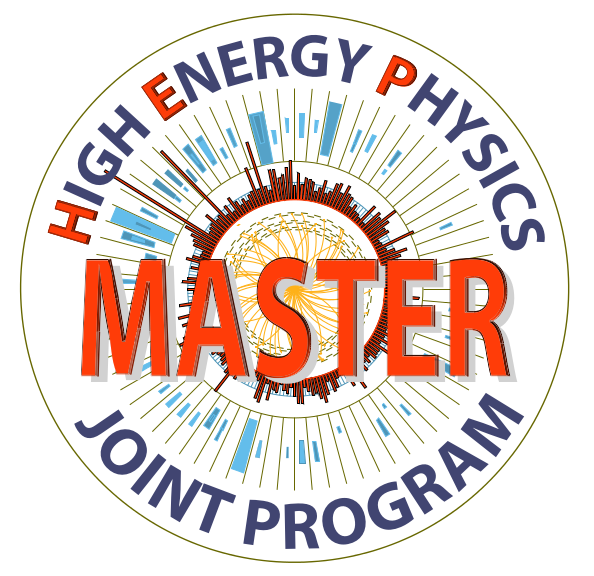
\includegraphics[scale=0.2]{Logos/logo_hep_centre_texte_coupe.png}
\end{flushright}
\end{minipage}

\end{figure}
\center
\HRule \\[0.4cm]
{ \huge \bfseries  Improving the reconstructed 4b signal final state pairing efficiency to Higgs boson candidate in the HH to 4b analysis at CMS
 \\[0.15cm] }
 \HRule \\[0.5cm]
 \center 
\textsc{\LARGE\textbf{Master Thesis}}\\[1cm]
{\Large ETH Zurich}\\[0.5cm]
{\Large CMS}\\[1cm]

{\large\textbf{Supervisor: Alessandro Calandri, Mauro Donegà}}\\[1cm]
Author: Ruth AMELLA RANZ\\
M2 High Energy Physics
\\[1cm]
\textbf{Abstract}\\[1cm]
\justifying
The Higgs boson is the last building block of the Standard Model (SM) of particle physics. Its discovery in 2012 by the ATLAS \cite{ATLASdecouvhiggs} and CMS \cite{CMShiggsdecouv} experiments represents a major breakthrough in particle physics as it proves the existence of a scalar field, with which the particles in the SM interact to gain their mass. Nevertheless,  there is an ongoing experimental effort to further probe the properties of the Higgs boson, for instance, the self-coupling constant $\lambda$. This can be probed in di-Higgs (HH) production. In this thesis, the use of SPANet \cite{SPANet}, an attention-based neural network is proposed for the HH $\to$ 4b analysis. 

\end{titlepage}

\newpage
\pagenumbering{gobble}
\tableofcontents
\pagenumbering{arabic}
\pagestyle{fancy}
\fancyhf{}
\fancyhead[L]{\rightmark}
\fancyfoot[C]{\thepage}
\setlength{\headheight}{13.59999pt}
\addtolength{\topmargin}{-1.59999pt}
\setlength{\headheight}{25.22153pt}
\addtolength{\topmargin}{-11.62154pt}

\newpage

\section{Introduction} \label{intro}

The unification of the electromagnetic and weak forces leading to the Electroweak force was experimetally verified by the discovery of the Z boson in 1983 at the Super Proton Synchrotron (SPS) at CERN. Nevertheless, although in this theory the gauge bosons $W^\pm$ and Z are considered to be massless, the experimental results proved the opposite. To explain the mass of these particles, we need to introduce the Higgs field, as via the Brout–Englert–Higgs mechanism these gauge bosons can acquire mass.

Explain better the Higgs flied and the potential and so on. The Higgs boson is excitation of this field. It's discovery proves the existence of a fundamental scalar sector in the SM.

%Nowadays the Higgs boson mass measured by the CMS experiment is 125.53 GeV with a precision of 0.15 GeV (cite). To further characterize this particle, there is an ongoing experimental effort to determine the value of the self-coupling $\lambda$, which will also allow to probe the shape of the scalar potential of the Higgs mechanism.

\section{The LHC and the CMS detector} \label{section: CMS}

% Add LHC

The Large Hadron Collider (LHC) is currently the largest and highest-energy particle accelerator. It is a 27-km long circular hadron accelerator located 100 meters underground at CERN, near Geneva, on the border between France and Switzerland. Protons are accelerated and collide every 25 ns at the four interaction points, corresponding to the four main experiments: ATLAS \cite{ATLAS}, CMS \cite{CMS}, LHCb \cite{LHCb}, and ALICE \cite{ALICE}. Figure \ref{fig: LHC} shows the  LHC complex as well as the location of the four main experiences.

\begin{figure}[hbt]
    \centering
    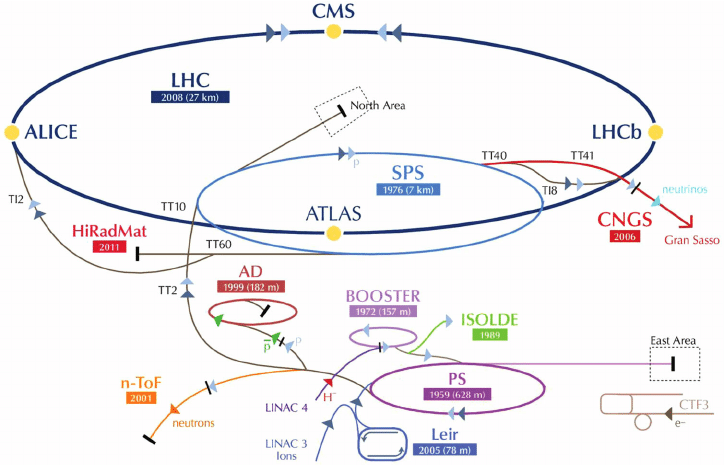
\includegraphics[width=0.6\linewidth]{Images/3.CMS/Existing-CERN-accelerator-complex-with-Large-Hadron-Collider-LHC-Super-Proton.png}
    \caption{The Large Hadron Collider (LHC) complex \cite{LHCFIG}.}
    \label{fig: LHC}
\end{figure}

Ever since the LHC started taking data, there have been 3 periods of data taking each one referred to as "Run". Figure \ref{fig: Runs} shows the integrated luminosity of the three periods of data taking (Run 1, 2, and 3) as well as the center of mass energy of the collisions $\sqrt{s}$ in each period. The integrated luminosity \lumi is the integral of the luminosity with respect to time:

\begin{equation}
    \lumi= \int \frac{1}{\sigma} \frac{dN}{dt} dt
\end{equation}

\noindent where $\sigma$ is the cross-section and $N$ the number of events detected.

\begin{figure}[hbt]
    \centering
    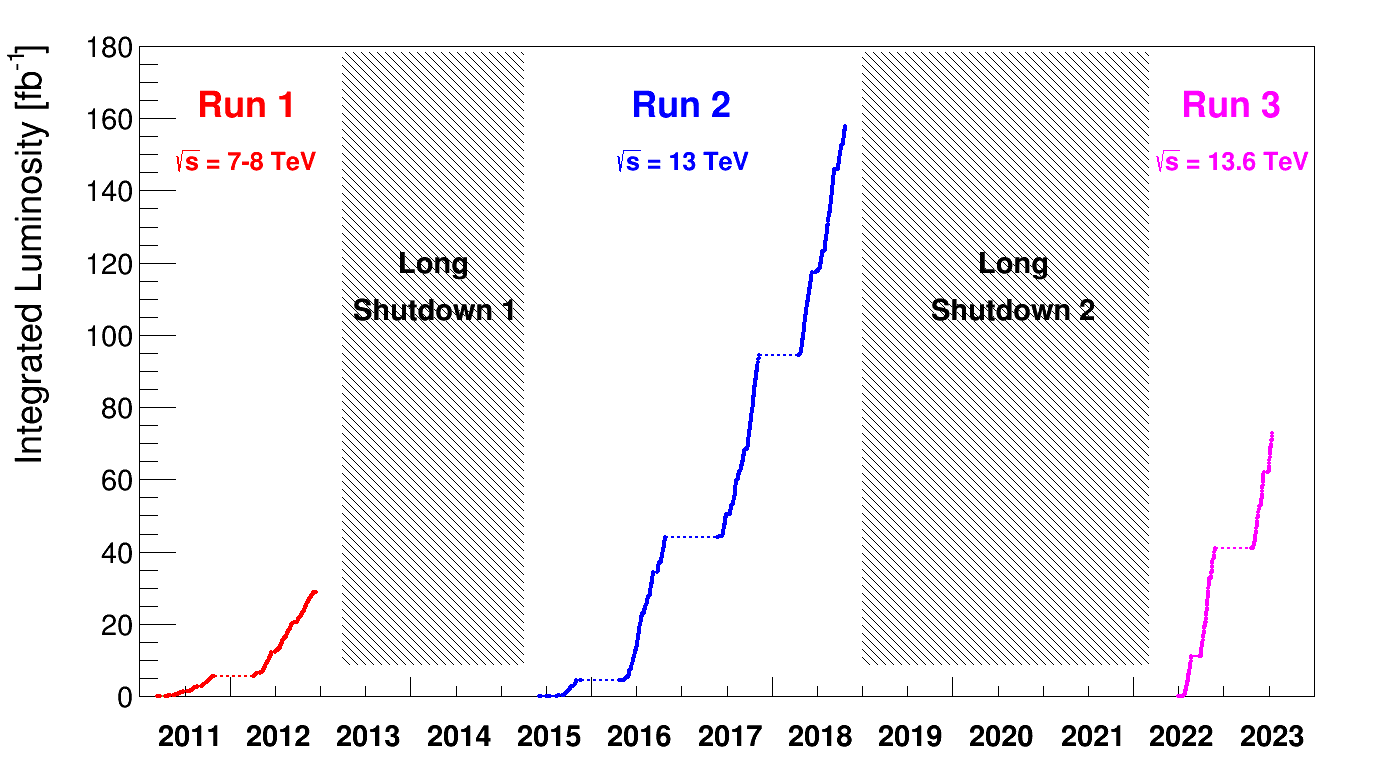
\includegraphics[width=0.5\linewidth]{Images/3.CMS/Run plots.png}
    \caption{Integrated luminosity delivered by LHC as a function of data-taking years. The center of mass energy of the collisions $\sqrt{s}$ is also reported \cite{Runplot}.}
    \label{fig: Runs}
\end{figure}

%https://be-dep-op-lhc.web.cern.ch

%explain run 2 and 3

CMS (Compact Muon Solenoid) is one of the four detectors of the LHC. It is made of (starting from the center) a tracker, made of silicon sensors, that can measure the trajectory of the particles. Then, to measure the energy of the electrons and the photons, the electromagnetic calorimeter (ECAL) is used. The latter stops these particles completely via interactions (showers) with the PbWO$_4$ crystals. ECAL is surrounded by HCAL, the hadron calorimeter, which stops the hadrons and reconstructs their energy. This is followed by a large superconducting magnet, inducing a very strong magnetic field (3.81 T), that bends the trajectory of the particles. This allows to retrieve information in the tracker about the momentum and the sign of the charge of the particle due to the bending of its trajectory by the magnetic field. The last layer of the detector is the muon detector. Figure \ref{fig: CMS detector} shows the different layers of the CMS detector. 

\begin{figure}[hbt]
    \centering
    \includegraphics[width=0.8\linewidth]{Images/3.CMS/cms_160312_02.png}
    \caption{A three-dimensional view showing the different layers of the CMS detector \cite{CMS3D}.}
    \label{fig: CMS detector}
\end{figure}

Collisions in the detector take place every 25 ns, to retrieve the information from the collisions, CMS uses a multi-level trigger system. The CMS trigger system consists of:
\begin{itemize}
    \item Level 1 (L1) trigger: this trigger is implemented using FPGAs (Field Programmable Gate Array) and ASICs (Application-Specific Integrated Circuit) and allows for a fast readout of the detector with limited granularity. \cite{L1Trigger}
    \item High Level Trigger (HLT): the events that are accepted by the L1 trigger are passed to the HLT. This trigger is implemented as software algorithms that run on large clusters of commercial processors. \cite{HLT}
\end{itemize}

Figure \ref{fig: coord syst} shows the 3D coordinate system of the CMS detector. The accelerated proton beams are along the $z$-axis and the collisions occur at the interaction point (IP). The $xy$-plane as is observed in Figure \ref{fig: coord syst} is the transverse plane.

\begin{figure}[hbt]
    \centering
    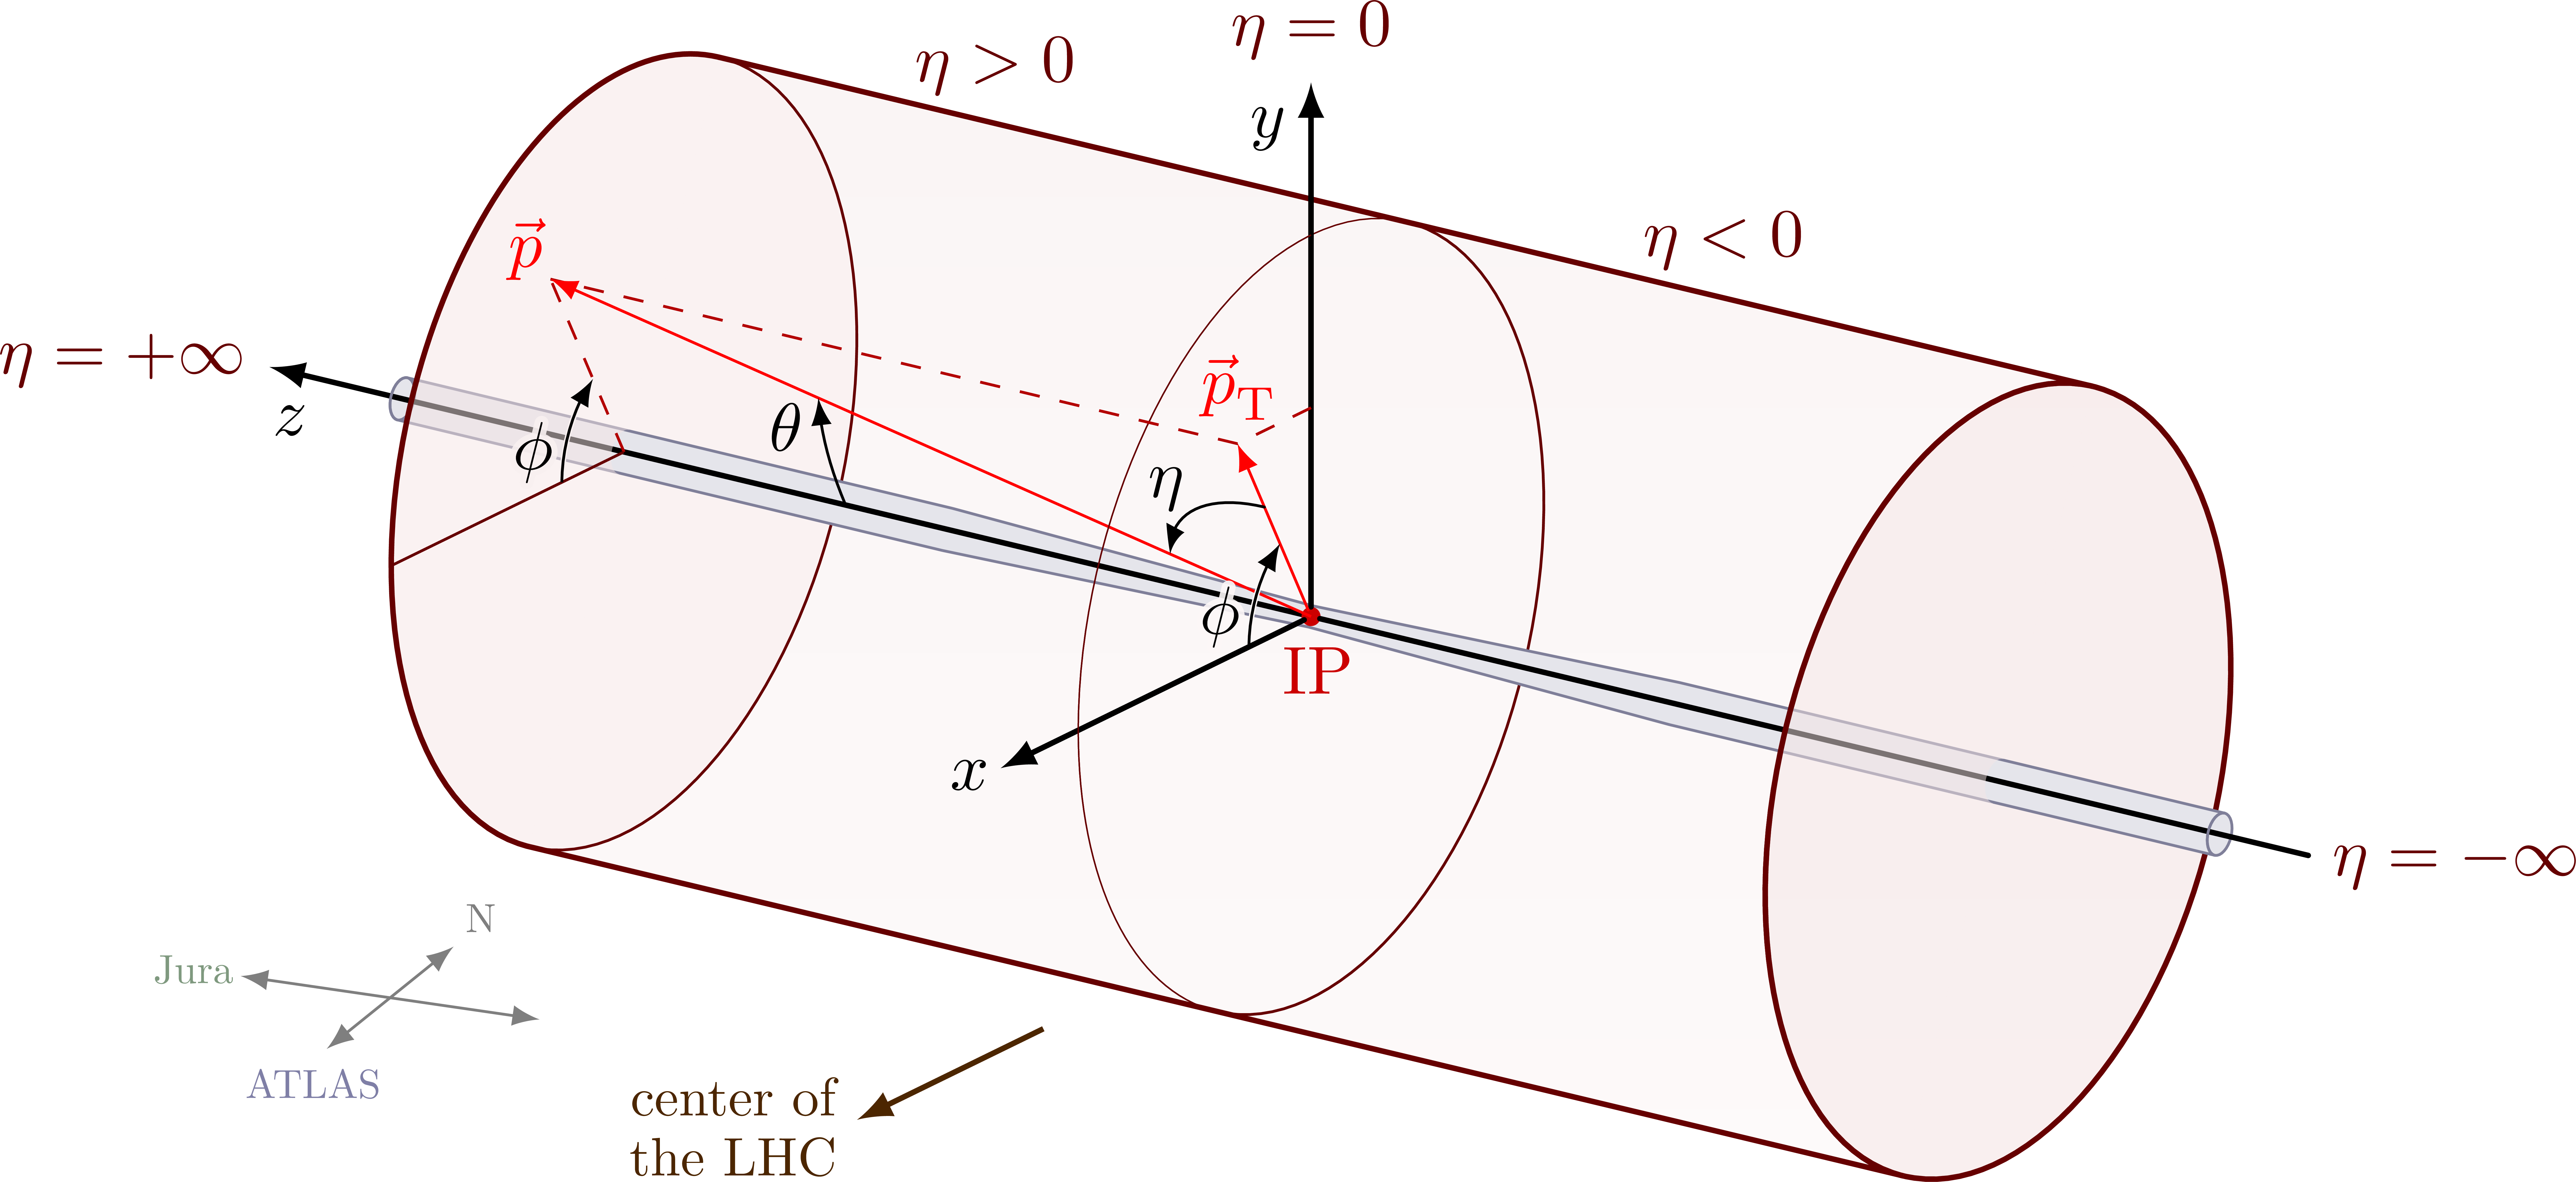
\includegraphics[width=0.7\linewidth]{Images/4.HH4b Analysis/axis3D_CMS-005.png}
    \caption{Coordinate system of the CMS detector \cite{CMScoord}.}
    \label{fig: coord syst}
\end{figure}

\subsection{Kinematic variables used in the HH $\to$ 4b analysis} \label{subsection: kinematic vars}
The definitions of the observables that will be used in the following Sections are reported in this Section. Figure \ref{fig: coord syst} shows the CMS coordinate system.

\begin{itemize}
    \item The pseudorapidity $\eta$, defined as:
    \begin{equation}
        \eta=-\mathrm{ln}\bigg(\text{tan}(\frac{\theta}{2})\bigg)
    \end{equation}
    with $\theta$ being the angle between the beam axis ($z$) and the deviated particle or jet. When the deviation is low, the pseudo-rapidity either tends to $\pm \infty$ depending on whether it is along the $z$-axis or in the opposite direction (see Figure \ref{fig: coord syst}).
    \item $\Phi$ is the azimuthal angle in the $xy$ plane. Since this angle is in the transverse plane it is Lorentz-invariant.
\end{itemize}

Since the physics processes should not depend on the reference frame, the $\eta, \Phi$ is the metric used in the detector since $\Delta \eta$ and $\Phi$ is Lorentz-invariant. 

\begin{itemize}
    \item Transverse momentum of the particles \pt: projection of the momentum in the transverse plane, as shown Figure \ref{fig: coord syst}. In proton-proton collisions, the colliding partons carry a fraction of z-momentum that depends on the parton distribution functions (PDF), leading to a boost of the particles. To avoid this, the transverse momentum is used. 
    \item $\Delta R$ is the angular distance between two objects, for instance, jets. It is defined as:
    \begin{equation}
        \Delta R = \sqrt{(\Delta \eta)^2 + (\Delta \Phi)^2 }
    \end{equation}
    \item \Ht is the sum of all the \pt of the jets in a given reconstructed event.
    \item b-tagging is the identification (tagging) of jets containing the decay of a B hadron (b jets). The ParticleNet tagger (PNet), initially introduced in \cite{PNet},
    is used to identify the flavor of the jet (b-, c-, light-flavour jets or gluon jets). Thus, this network provides a score (b-tag score) which is correlated to the probability of a jet to originate from a b-quark, a c-quark or a light-flavor quark. The closer the score is to one, the more likely it is to be a jet originating from a b quark. Three working points (WPs) are defined:
    \begin{itemize}
        \item Tight WP: 0.1\% of misidentification (mistagging) of the flavor of the jet, i.e. only 0.1\% of the events above this point are jets coming from a quark with a lighter flavor or a gluon but are classified as b jets.
        \item Medium WP: 1\% of misidentification of the flavour of the jet
        \item Loose WP: 10\% of misidentification of the flavor of the jet
    \end{itemize}
    \item \pt regressed (\pt reg): by using the ParticleNet neural network it is possible to correct the raw jet \pt to the generator-level jet energy. To do so, two components are taken into account: the \pt is adjusted to be closer to the generator-level jet \pt, and the presence of neutrinos, not reconstructed in the detector, is also taken into account, by summing their transverse momentum to the jet.
    \item Impact parameter $d_0$ is the distance of closest approach between the daughter particle trajectory and the mother particle production point. The impact parameter (IP) is shown in Figure \ref{fig: IP}. The impact parameter in the $xy$ plane is noted $d_{xy}$ and along the z-axis $d_z$.
\end{itemize}

\begin{figure}[hbt]
    \centering
    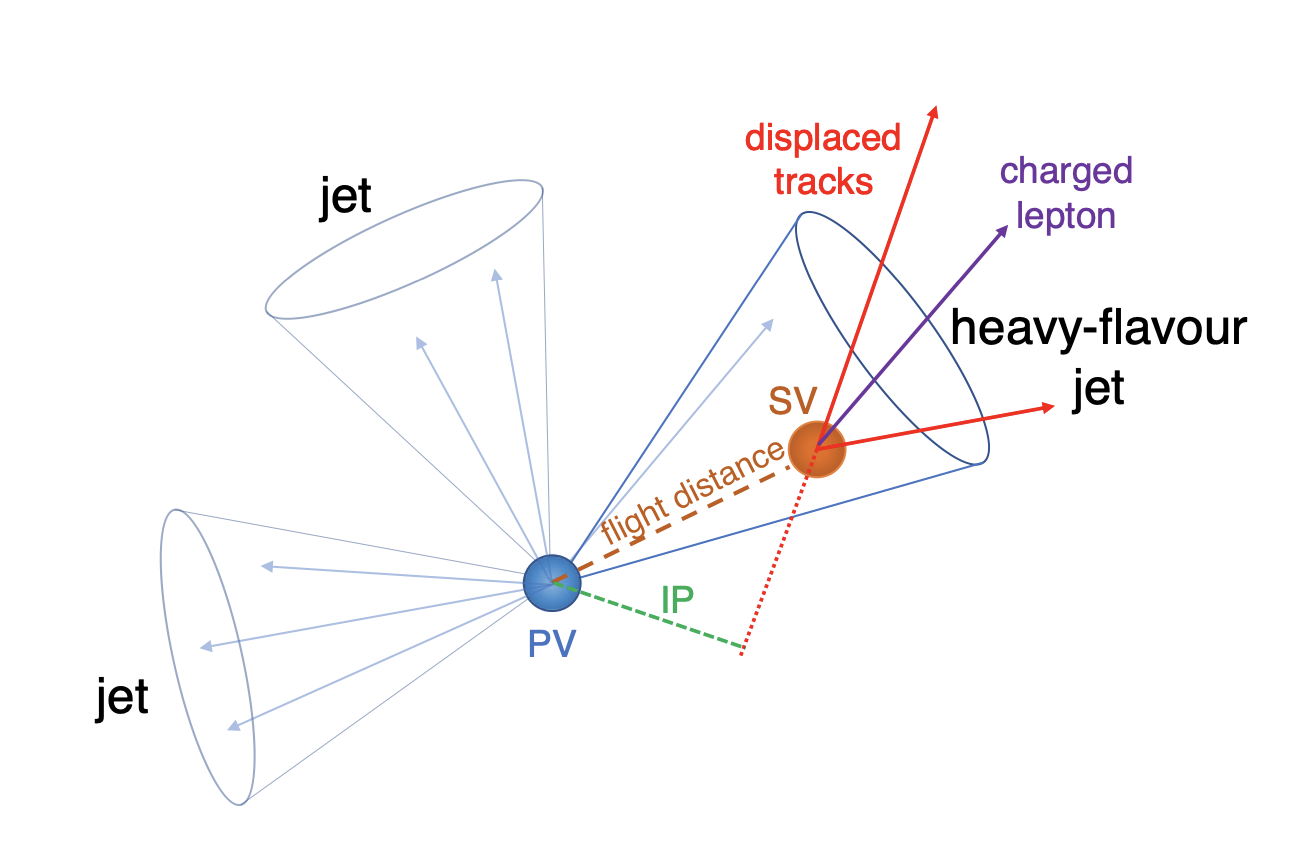
\includegraphics[width=0.5\linewidth]{Images/3.CMS/impact parameter.png}
    \caption{Sketch showing the definition of the impact parameter (IP) as well as primary (PV) and secondary (SV) vertices in heavy-flavor jet production \cite{IP}. }
    \label{fig: IP}
\end{figure}


%Maybe nno need of too much on this part

% \subsection{Tracker}
% \subsection{Electromagnetic calorimeter (ECAL)}
% \subsection{Hadronic Calorimeter (HCAL)}
% \subsection{Solenoid}
% \subsection{Muon detector}
% \subsection{Triggers}
% \subsection{Event recontsruction}
% \subsubsection{Primary Vertex}
% \subsubsection{Pile-up}
% \subsubsection{Jet reconstruction}
% \subsubsection{Missing Energy}
% \subsubsection{B-tagging} \label{Btagging} b tag algorithms are used and the fact that we use th e btag fpr the morphing to 2b to 4b
% \subsubsection{pt reg} \label{subsubsec: btag-ptreg}
% The \pt regressed is the one computed using a DNN. The main idea is that, we train a DNN with information from the reco jets and we try to retrieve the original energy if these jets. For efficiency purposes this DNNN gives out the ratio of the predicted E/ original E. To improve the analysis, we use \pt reg, which means that we multiply the \pt measured by the detector times this ratio, which allows us ti have a more precise value of thee \pt of the objects we are using.
% \subsection{Monte-Carlo}
% \subsubsection{Gen/Reco jets}

% 0.1 perccent if misidentification if the flaviur
% 1
% 10

\section{Presenting the HH to 4b analysis, maybe mention cross sections and so on} \label{section: HH4b}

\subsection{Goal}

Signature and goal

\subsection{Presenting the cutflows for this analysis} \label{subsection:cutflows}
To train our SPANet model we are working with Monte-Carlo simulations. 

explain 2b/4n

This dataset contains data collected in 2022, during the Run 3 and we require that the mean PNet of the leading 2 b-tag jets > 0.65, and the 3° and 4° PNet b-tag < 0.2605 (medium WP). By imposing this requirement, we know that in this dataset there are very little signal events, 

\subsection{Signature}

Goal: Parametr lambda of the Higgs potential, affects the trilinear Higgs coupling . Study HH production is the only way to directly probe the H boson self coupling 

Production modes: gluon fusion (add cross section and cite AN)/ VBF

H -> 4b bc this decaying has the highest BR

\subsection{Presenting the run 2 analysis method}

\subsubsection{Signal and control regions}
\subsection{New pairing method}

In order to improve the pairing done using the Run 2 method we want to use the attention-based neural network SPANet, whose architecture will be presented in section \ref{section: spanet architecture}. As we previously mentioned, we are interested in the decay of two Higgs Boson particles into 2 b quarks respectively. Therefore, in the final state we want at least 4 jets that we want to match to the original b quarks coming from the Higgs' decay. However, even if our process should have 4 jets in the final state, due to pile-up or other QCD processes, we can have more than 4 jets in the final state. In order to identify our signal, we can use btagging, presented in section \ref{Btagging}.


Nevertheless, because of the pile-up in the detector and other QCD processes, we can have more than 4 jets in the final state. However, as we are interested in jets originated by b quarks, these have particular signature and can be differentiated from jets originated by other quarks or gluons. This process is called b-tagging.

We will be working with Montecarlo simulations for our signal of interest. \textbf{Need more info on this}. Idk maybe also explain gen vs reco jets , but maybe this has to be done before.


\section{SPANet and Machine Learning} \label{section: spanet architecture}





\section{Improving the pairing efficiency with SPANet}


\subsection{Choice of the optimal inputs for the training}
As mentioned in section \ref{section: spanet architecture} we can give SPANet global and sequential inputs for the training. The sequential inputs being the ones that can have an arbitrary number of vectors per event, they will correspond to the information of the jets used for the pairing. On the other hand, the global vectors are the ones that will have a single vector per event, so they correspond to event level information.

In order to find the optimal training that maximizes our pairing efficiency, we started by testing different configurations. As precised before, we want 4 jets in the final state, nevertheless due for instance to QCD processes even if in an event there is di-Higgs production decaying into 4 b quarks, we can have more than 4 jets in the final state. Hence, we want to start by checking how much do we gain in signal efficiency by considering other jets in the final state with lower b-tag score for the pairing. This can be seen in Table \ref{table:signal_efficiency}. We first present the percentage of signal where the $k^{th}$ jet was matched, meaning that this $k^{th}$ jet was matched to one of the gen jets. We also show the percentage of signal of fully matched events, meaning the events for which 4 jets are matched to the 4 gen jets. Out of the total number of events 92.9\% are fully matched and the percentage of fully matched events when considering the first 4 leading jets is 90.2\%. According to Table \ref{table:signal_efficiency}, we can see that most of the remaining signal efficiency is gained by considering a fifth jet for the paring (we gain 2.5\% out of 2.7\%). 

From these results, we conclude that the highest signal efficiency is obtained by considering either 4 or 5 jets for the pairing. Therefore, we will train SPANet using 4 and 5 jets as sequential inputs. We will also make one test considering 6 jets as sequential inputs, nevertheless this did not increase our performance, hence the choice of stopping at 5 jets for the pairing.


\begin{table}[h!]
\centering
\begin{tabular}{|p{1cm}||p{6cm}||p{6cm}|}
 \hline
 k  & Percentage of the signal with the $k^{th}$ jets matched & Percentage of signal fully matched events with the $k^{th}$ jet matched\\
 \hline
 4 &  94.4 & 90.2\\
 5 & 2.76 & 2.52 \\
 6 & 0.27 & 0.25 \\
 $\geq$7 &  $\approx$0.03 &  $\approx$0.02 \\
 \hline
\end{tabular}
\caption{Signal Efficiency}
\label{table:signal_efficiency}
\end{table}

For the first SPANet trainings, we will compare the performance of using either 4 or 5 jets as sequential inputs. We will use as first figure of merit for the performance the inclusive pairing efficiency and the \textit{total} pairing efficiency. We define the pairing efficiency as:

\begin{equation*}
    \text{Pairing efficiency}=\frac{\text{Correctly fully matched events}}{\text{Total number of fully matched events}}
\end{equation*}

However, as we explained earlier, the number of fully matched events is larger when considering a fifth jet for the pairing, hence to have a fair comparison between the trainings we need to compute the \textit{total} pairing efficiency which is given by:
\vspace{-0.2cm}
\begin{eqnarray*}
\text{Total efficiency} & = & \text{Pairing efficiency} \times \text{Fraction of fully matched events} \\
% & = & \frac{\text{Correctly fully matched events}}{\text{Total number of fully matched events}} \times \frac{\text{Total number of fully matched events}}{\text{Total number of events}} \\
& = &\frac{\text{Correctly fully matched events}}{\text{Total number of events}}     
\end{eqnarray*}

This is why in table \ref{table: First comparison} we summarize these first results by showing the configuration of the training as well as the pairing efficiency and for a fair comparison, the total pairing efficiency.

\begin{table}[h!]
\centering
\begin{tabular}{|M{2cm}|M{5cm}|M{2cm}|M{2cm}|M{2cm}|}
 \hline
 Training  & Configuration &  Pairing efficiency & Fraction of fully matched events & Total pairing efficiency \\
 \hline
 4 jets &  \raggedright 4 jets considered for the pairing and using \begin{itemize}[itemsep=0.01em]
    \item \pt
    \item $\eta$
    \item $\phi$
    \item b-tag
 \end{itemize} 
 as kinematic information & 0.984 & 0.901 & 0.887 \\
 \hline
 4 jets 5 global & \raggedright 4 jets considered for the pairing and a 5$^{\text{th}}$ given as global information. We use \begin{itemize}[itemsep=0.01em]
    \item \pt
    \item $\eta$
    \item $\phi$
    \item b-tag
 \end{itemize} 
 as kinematic information  & 0.984 & 0.901 & 0.887\\
 \hline
  5 jets & \raggedright 5 jets considered for the pairing and using \begin{itemize}[itemsep=0.01em]
    \item \pt
    \item $\eta$
    \item $\phi$
    \item b-tag
 \end{itemize} 
 as kinematic information &  0.942 & 0.926 &  0.872 \\
 \hline
\end{tabular}
\caption{Comparison of the efficiency of the first trainings}
\label{table: First comparison}
\end{table}

As explained in the beginning, the global variables only add event level information, therefore in the training using 4 jets 5 global, the fifth jet adds information of kinematics of the system but is not used for the pairing.

From the results shown in Table \ref{table: First comparison}, we can at first say that using this configuration of the trainings, using 4 jets and 5$^{\text{th}}$ global or 4 jets as inputs are more performing. Nevertheless, by considering a 5$^{\text{th}}$ jet as either a global input or for the pairing can help the network as it has more information about the event, therefore, before stopping the trainings using 5 jets, we will try different configurations using 4 jets with a 5$^{\text{th}}$ global and 5 jets as inputs.


In Tables \ref{table:5 jets trainings} and  \ref{table:4 jets trainings}, we show the different configurations for the new trainings as well as their performance. In the new configurations we either vary the kinematical information of the jets or some of the hyperparameters of the model. In the first trainings presented earlier we used what we will call the \textit{Large model}, that uses the default SPANet hyperparameters. However, we wanted to try some of the hyperparameters shown in \textbf{cite}, and this configuration will correspond to the \textit{Lite Model}. The comparison of these models is shown in Table \ref{table:comparison_models}.

\begin{table}[h!]
    \centering
     \begin{tabular}{|c||c|c|}
      \hline
         & Large model &  Lite model\\ 
      \hline
      Hidden dimensions & 64 &  32\\ 
      \hline
      Transformer dimension& 64 & 64 \\ 
      \hline
      Embedding layers & 10 & 8 \\ 
      \hline
      Encoder layers & 6 & 6 \\ 
      \hline
      Trainable parameters & \textbf{2.2 M} & \textbf{0.5M} \\ 
      \hline
      Learning rate & 0.0015 & 0.00659 \\ 
      \hline
      Batch size & 2048 & 2048 \\ 
      \hline
      Optimizer & AdamW & AdamW \\ 
      \hline
      Number of epochs & 50 & 50 \\
      \hline
    \end{tabular}
    \caption{Comparison of Large and Lite Models}
    \label{table:comparison_models}
\end{table}


\begin{table}[h!]
\centering
\begin{tabular}{|M{2.5cm}|M{5.25cm}|M{1.75cm}|M{1.75cm}|M{1.75cm}|}
 \hline
 Training  & Configuration &  Pairing efficiency  & Fraction of fully matched events & Total pairing efficiency \\
 \hline
 5 jets & \raggedright \footnotesize \begin{itemize}[itemsep=0.001em]
    \item \pt
    \item $\eta$
    \item $\phi$
    \item b-tag
    \item Large model
 \end{itemize} & 0.942 & 0.926 & 0.872 \\
 \hline
 5 jets with b-tag preselection \pt regressed & \raggedright  \footnotesize \begin{itemize}[itemsep=0.001em]
    \item \pt
    \item $\eta$
    \item $\phi$
    \item b-tag
    \item Large model
    \item Fifth jet has a b-tag above the medium working point
 \end{itemize}  & 0.975 & 0.913 & 0.890 \\
 \hline
  5 jets \pt regressed and Lite model & \raggedright \footnotesize \begin{itemize}[itemsep=0.001em]
    \item \pt regressed
    \item $\eta$
    \item $\phi$
    \item b-tag
    \item Lite model
 \end{itemize} &  0.969 & 0.926 & 0.897\\
 \hline
 5 jets \pt regressed, Lite model and b-tag preselection & \raggedright \footnotesize \begin{itemize}[itemsep=0.001em]
    \item \pt
    \item $\eta$
    \item $\phi$
    \item b-tag
    \item Lite model
    \item Fifth jet has a b-tag above the medium working point
 \end{itemize} 
  & 0.977 & 0.913 & 0.892\\
 \hline
\end{tabular}
\caption{Different configurations for trainings with 5 jets as sequential inputs}
\label{table:5 jets trainings}
\end{table}

\begin{table}[h!]
\centering
\begin{tabular}{|M{2.5cm}|M{5.25cm}|M{1.75cm}|M{1.75cm}|M{1.75cm}|}
 \hline
 Training  & Configuration &  Pairing efficiency  & Fraction of fully matched events & Total pairing efficiency \\
 \hline
 4 jets 5 global & \raggedright \footnotesize \begin{itemize}[itemsep=0.001em]
    \item \pt
    \item $\eta$
    \item $\phi$
    \item b-tag
    \item Large model
 \end{itemize} & 0.984 & 0.901 & 0.887 \\
 \hline
 4 jets 5 global \pt regressed & \raggedright  \footnotesize \begin{itemize}[itemsep=0.001em]
    \item \pt regressed
    \item $\eta$
    \item $\phi$
    \item b-tag
    \item Large model
 \end{itemize}  & 0.985 & 0.901 & 0.887 \\
 \hline
  4 jets 5 global \pt regressed and Lite model & \raggedright \footnotesize \begin{itemize}[itemsep=0.001em]
    \item \pt regressed
    \item $\eta$
    \item $\phi$
    \item b-tag
    \item Lite model
 \end{itemize} &  0.986 & 0.901 & 0.888\\
 \hline
 4 jets 5 global Lite model & \raggedright \footnotesize \begin{itemize}[itemsep=0.001em]
    \item \pt
    \item $\eta$
    \item $\phi$
    \item b-tag
    \item Lite model
 \end{itemize}  & 0.983 & 0.901 & 0.886 \\
 \hline
 4 jets 5 global with b-tag preselection & \raggedright \footnotesize \begin{itemize}[itemsep=0.001em]
    \item \pt
    \item $\eta$
    \item $\phi$
    \item b-tag
    \item Large model
    \item Fifth jet given as global input has a b-tag above the medium working point
 \end{itemize} 
  & 0.984 & 0.901 & 0.886\\
 \hline
\end{tabular}
\caption{Different configurations for trainings with 4 jets as sequential inputs}
\label{table:4 jets trainings}
\end{table}

From Tables  \ref{table:5 jets trainings} and  \ref{table:4 jets trainings}, we can see that for both either 5 jets or 4 jets 5 global, the best performance is obtained by using \pt reg and the Lite model. However here we only compare the total pairing efficiencies inclusively, but it is also possible to plot them differential as a function of $m_{HH}$, as can bee seen in Figures \ref{fig: comp 4j5g} and \ref{fig: comp 5j}. In Figure \ref{fig: comp 4j5g} we can see that using different configurations for 4 jets and 5th global does not make impact much our total pairing efficiency. On the contrary, in Figure \ref{fig: comp 5j} we can see how much difference it makes to change the configuration of the training.


\begin{figure} [h!]
    \centering
    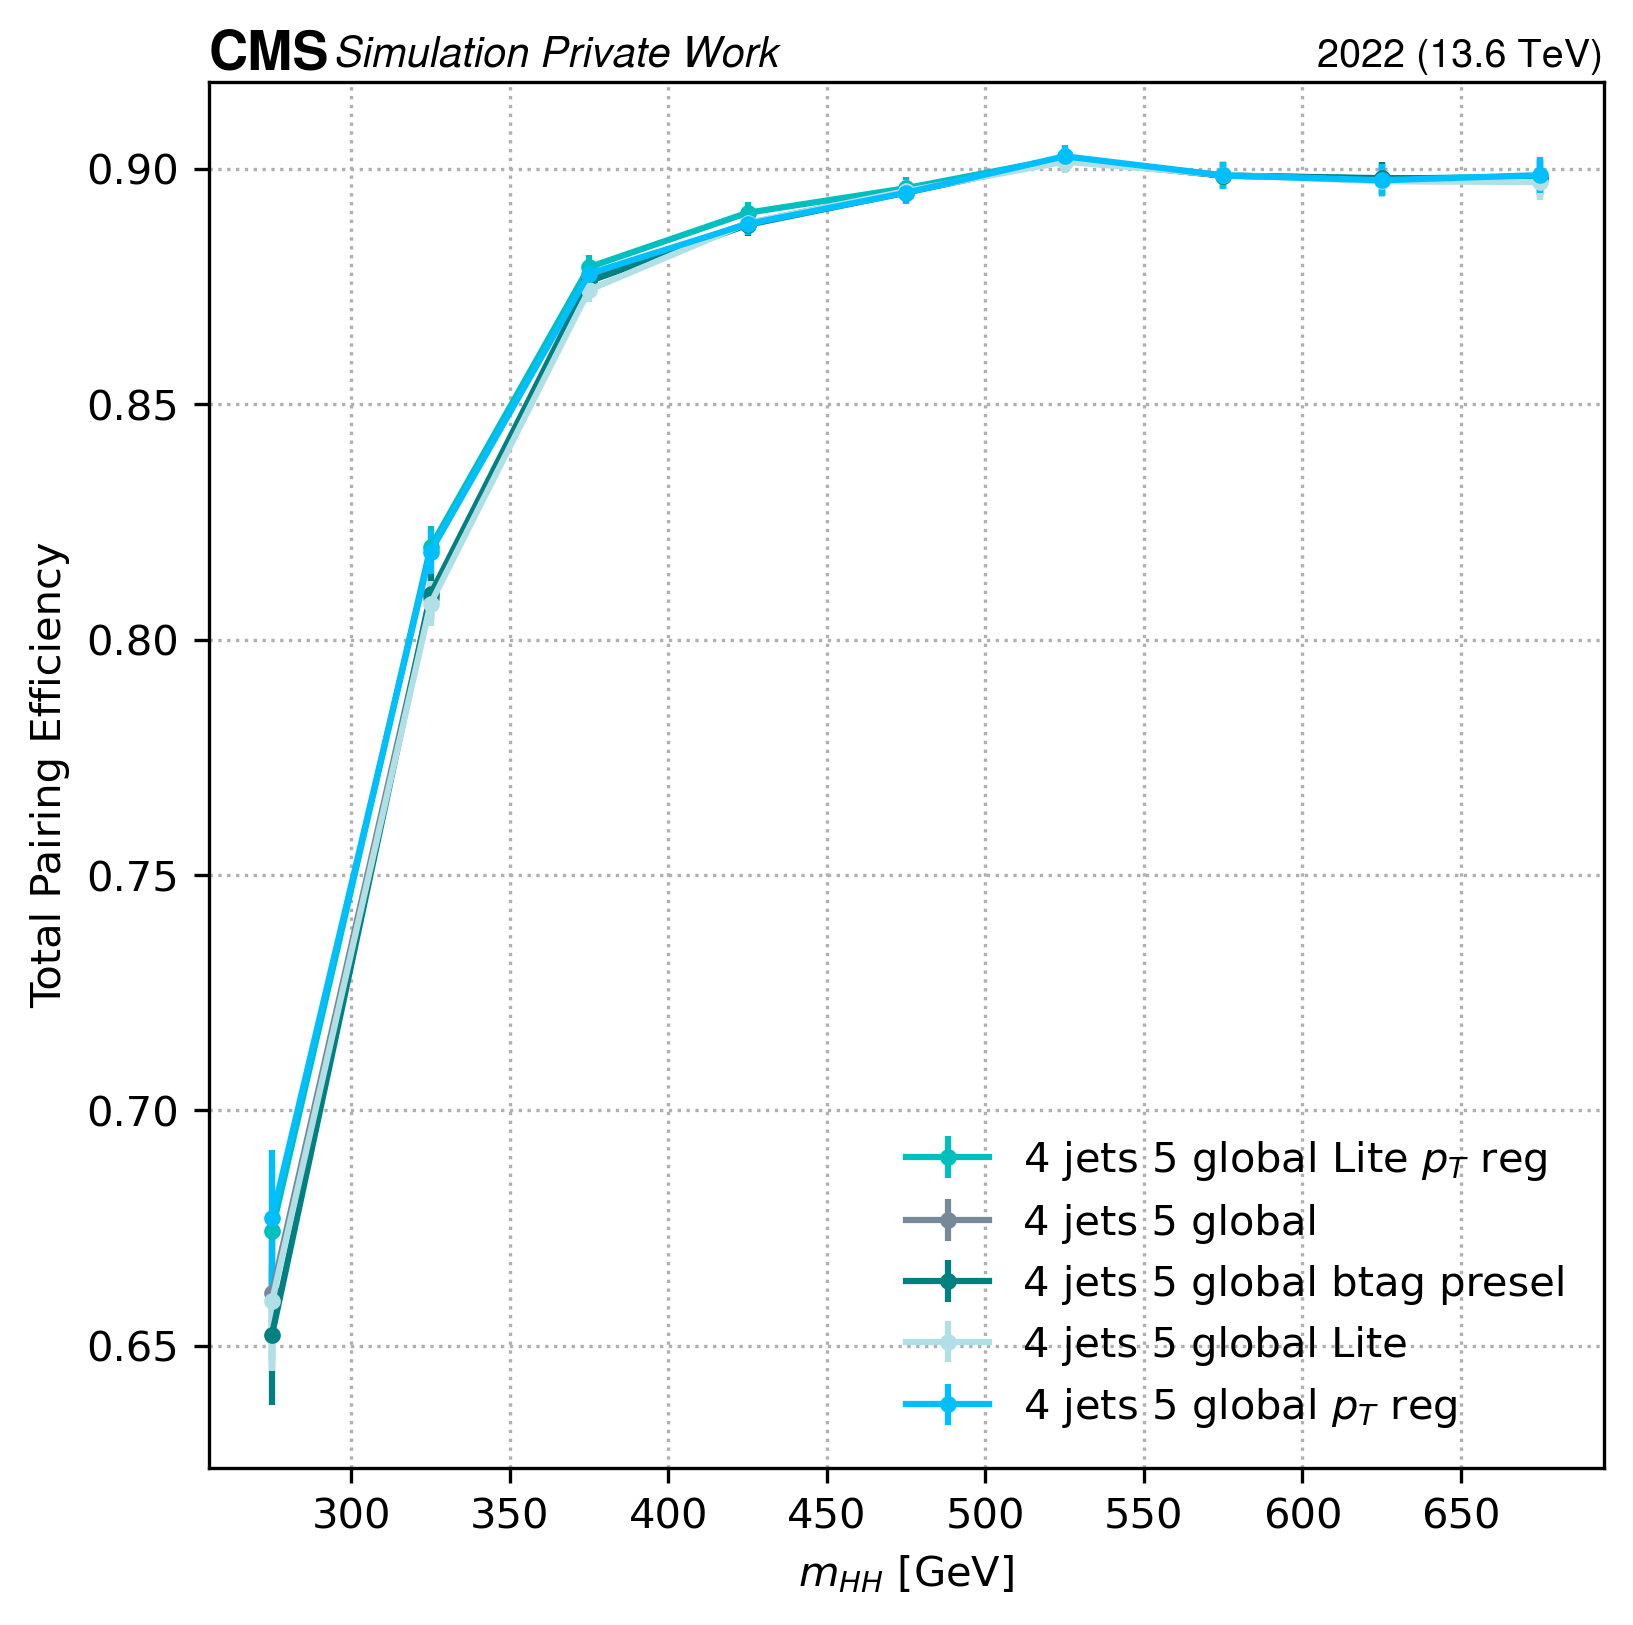
\includegraphics[width=0.6\linewidth]{Images/6.Improving/Imput Comparisons/4j5g training comp.png}
    \caption{Comparison of different trainings using 4 jets and a 5$^\text{th}$ global as input}
    \label{fig: comp 4j5g}
\end{figure}

\begin{figure}[h!]
    \centering
    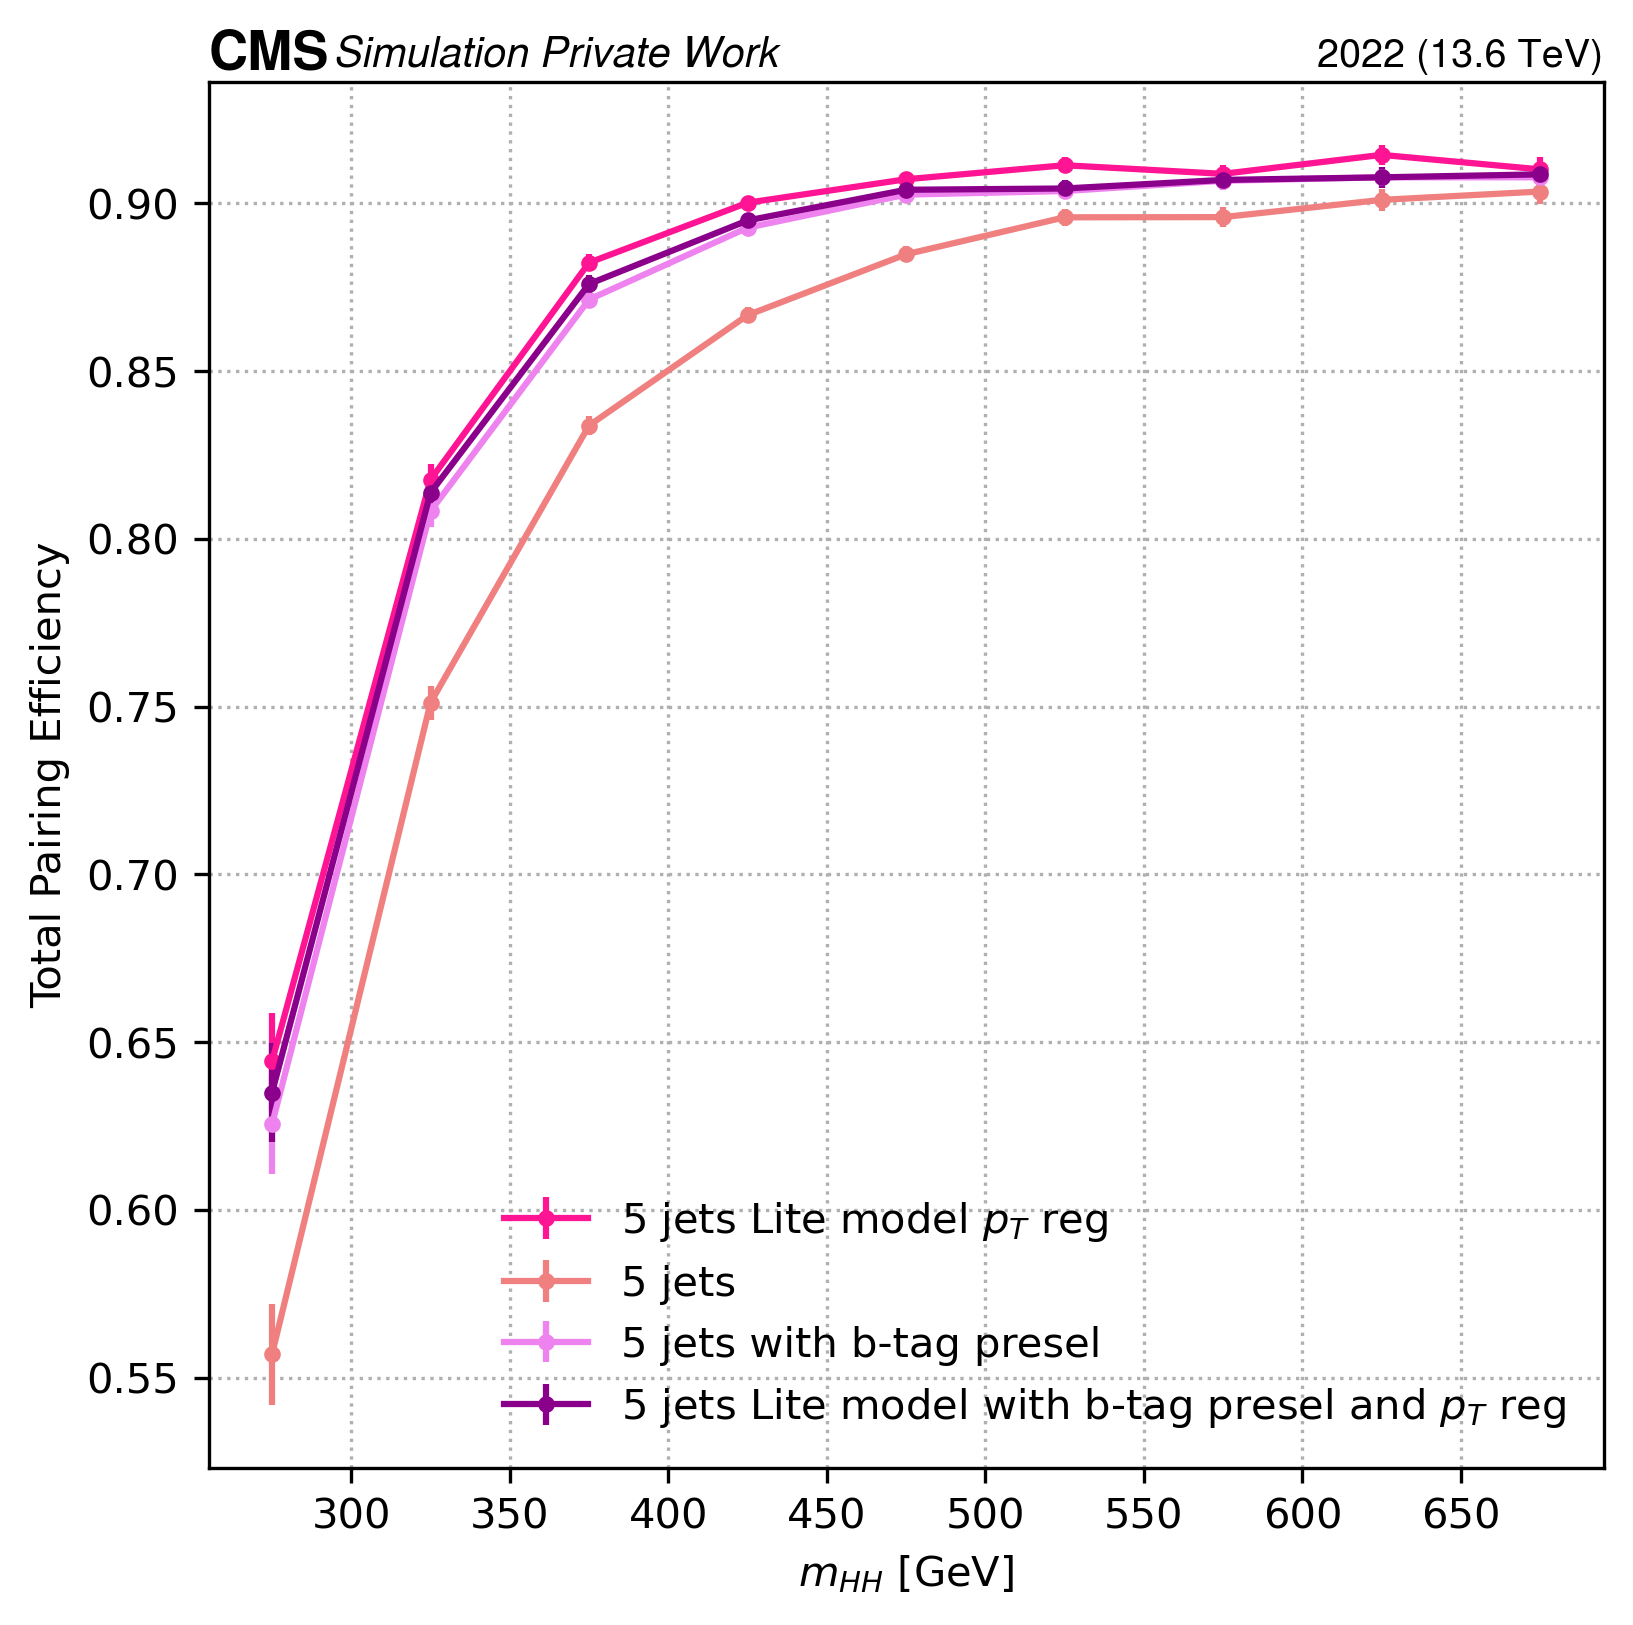
\includegraphics[width=0.6\linewidth]{Images/6.Improving/Imput Comparisons/5j training comp.png}
    \caption{Comparison of different trainings using 5 jets as inputs}
    \label{fig: comp 5j}
\end{figure}



The next step is to compare these two models to the performance of the $D_{HH}$-method presented in section \ref{section: HH4b}. The comparison is done for events for which we have $\Delta D_{HH} > 30$ GeV, as we only could implement this method for these events. In Figure \ref{fig: 2 best models comp} we show how these 2 models outperform the $D_{HH}$-method. 

\begin{figure}[h!]
    \centering
    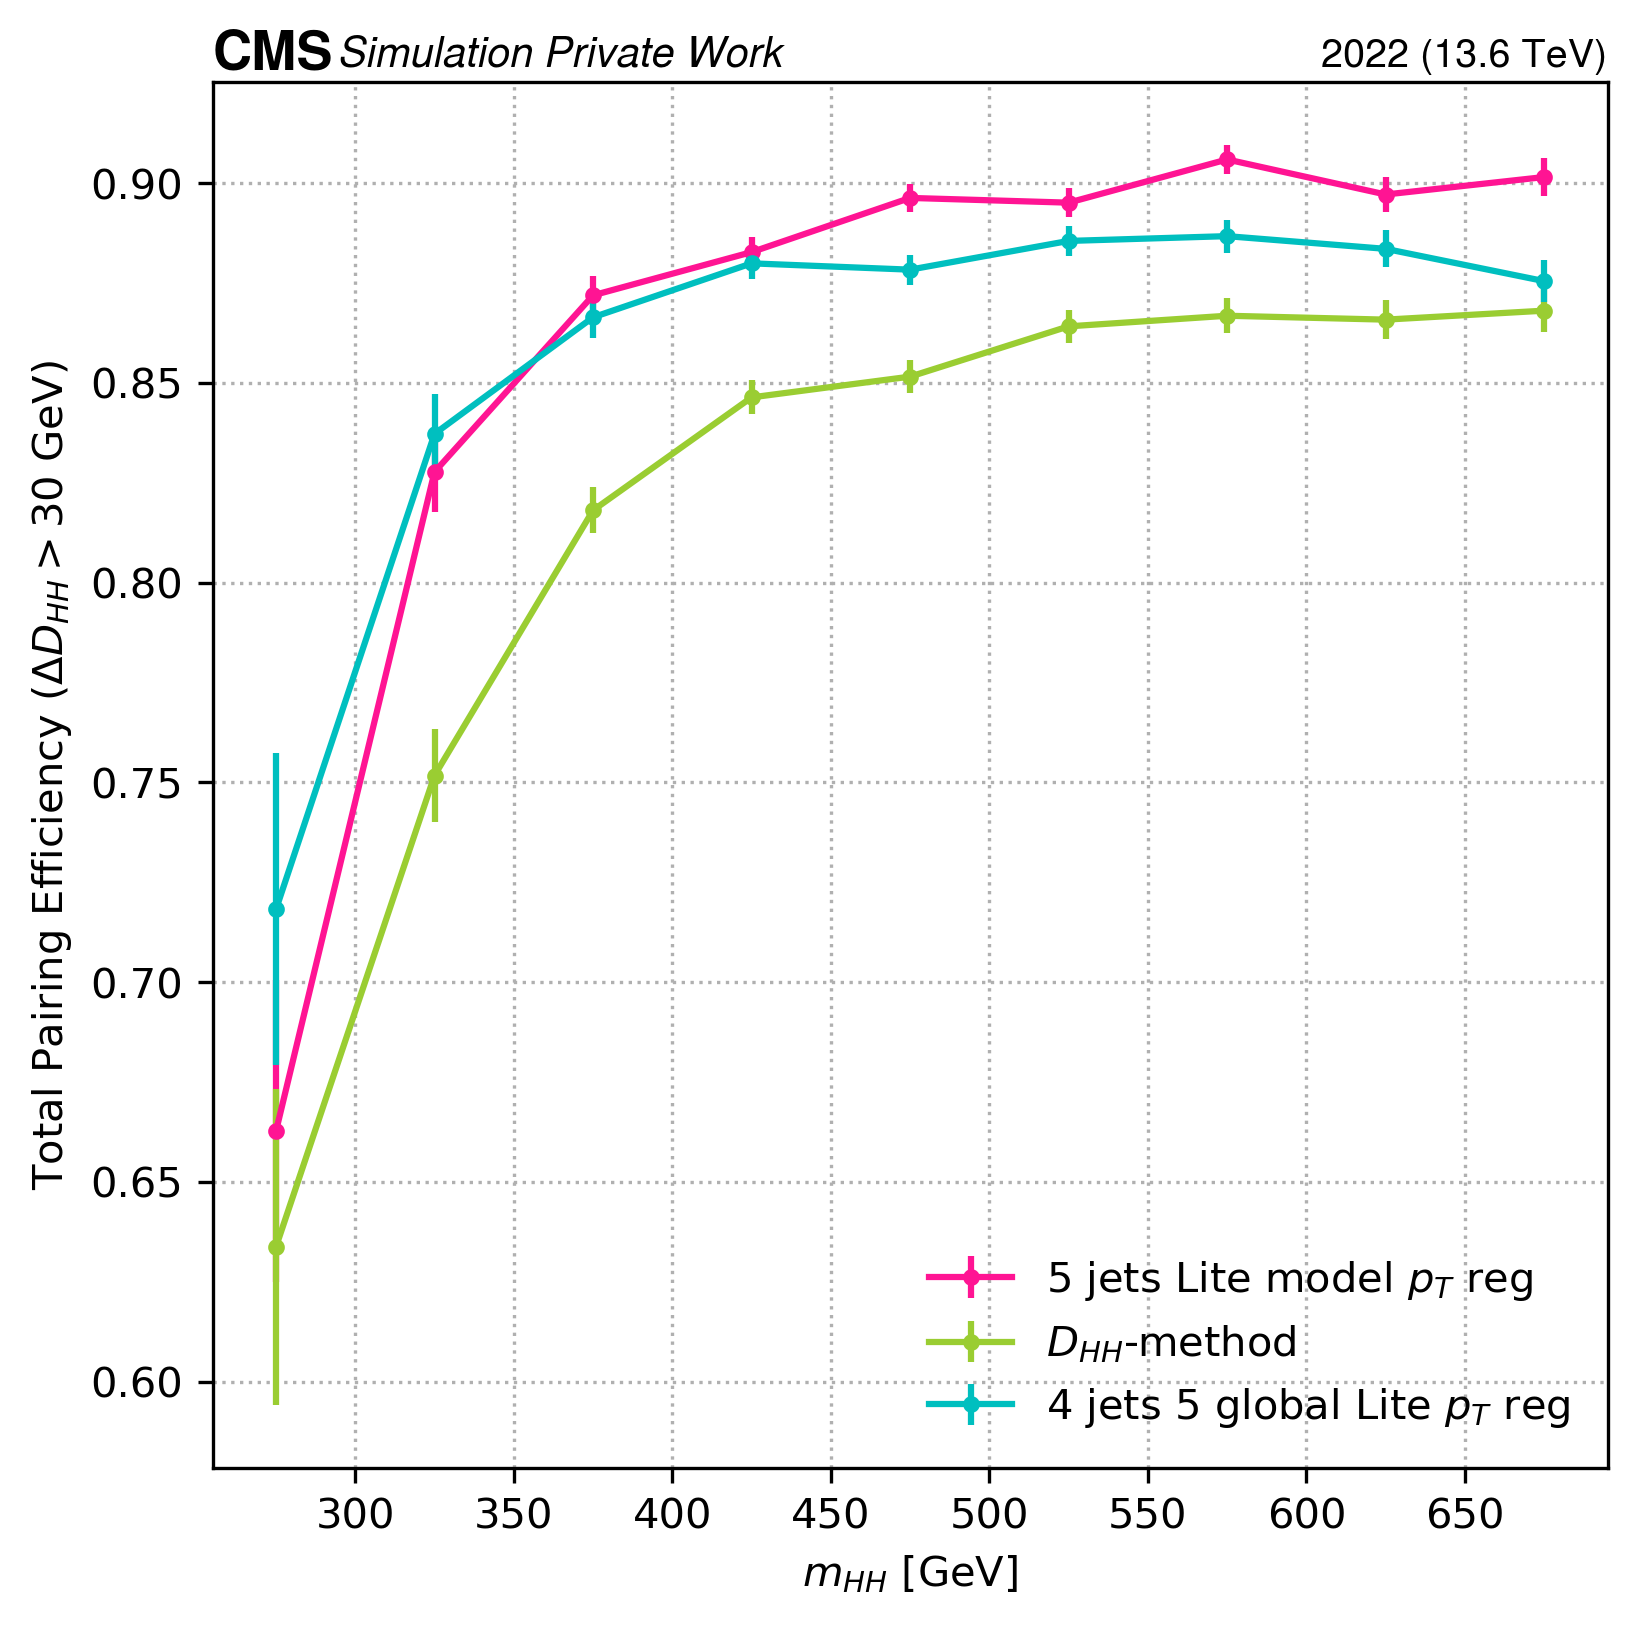
\includegraphics[width=0.6\linewidth]{Images/6.Improving/Imput Comparisons/2 best models comp run2 .png}
    \caption{Comparison of our two best performing models to the $D_{HH}$-method}
    \label{fig: 2 best models comp}
\end{figure}

\vspace{0.2cm}

\noindent In conclusion, we obtained 2 models:

\begin{itemize} [itemsep=0.1em]
    \item 4 jets as sequential inputs with a 5th global jet using the \pt reg $\eta, \phi$ and btag of the jets as well as the lite model
    \item 5 jets as sequential inputs using the \pt reg $\eta, \phi$ and btag of the jets as well as the lite model
\end{itemize}

\noindent which have the highest total efficiency and that outperform the pairing efficiency used in the $D_{HH}$-method.

We also tried to asses the performance of these trainings evaluated on datasets where we only have 4 jets, but these evaluations are not correct due to the difference of phase space between the train and the test files. Moreover, we performed a test by training without the b-tag of the jet as input, nevertheless the performance was much worse than by including it in the inputs.

Even though the training using 5 jets as inputs outperforms the training using 4 jets with a 5$^{\text{th}}$ global, as a next figure of merit to choose our optimal model, it is important to verify if when applying our model in data, we observe background mass sculpting.

\clearpage

\subsection{Background mass sculpting}
In addition to the pairing efficiency, another figure of merit we use in order to select the best model is the mass sculpting of the background. This is a very important feature as if we evaluate our model in a sample with mostly background events, we should not observe a fake peak of events around the signal region. 

To verify this, we will use the models we presented in the last section and evaluate them in a sample of 2b data. This dataset contains data collected in 2022 during the Run 3, and as explained in section \ref{subsection:cutflows} due to the requirements of the 2b region, we have mostly background events and the signal contribution due to mistagging of the jets is negligible. Hence, if we evaluate our model here, we should not observe a peak of events in the $m_{HH}$ plane around the signal region (defined in section \ref{section: HH4b}). Indeed, in Figure \ref{fig: 2D mass dist sig}, we show the 2D mass distribution of the evaluation of our model on signal events. We can see that most of the predicted events are in the signal region, as we would expect. Contrary, in Figures \ref{fig: 2D mass sculpting for 4j5g} and \ref{fig: 2D mass sculpting for 5j}, we show the 2D mass distribution of the evaluation of our best models on 2b data. We can see that there is not a peak of events in the signal region, which is indeed what we expected. 

\begin{figure}[hbt]
    \centering
    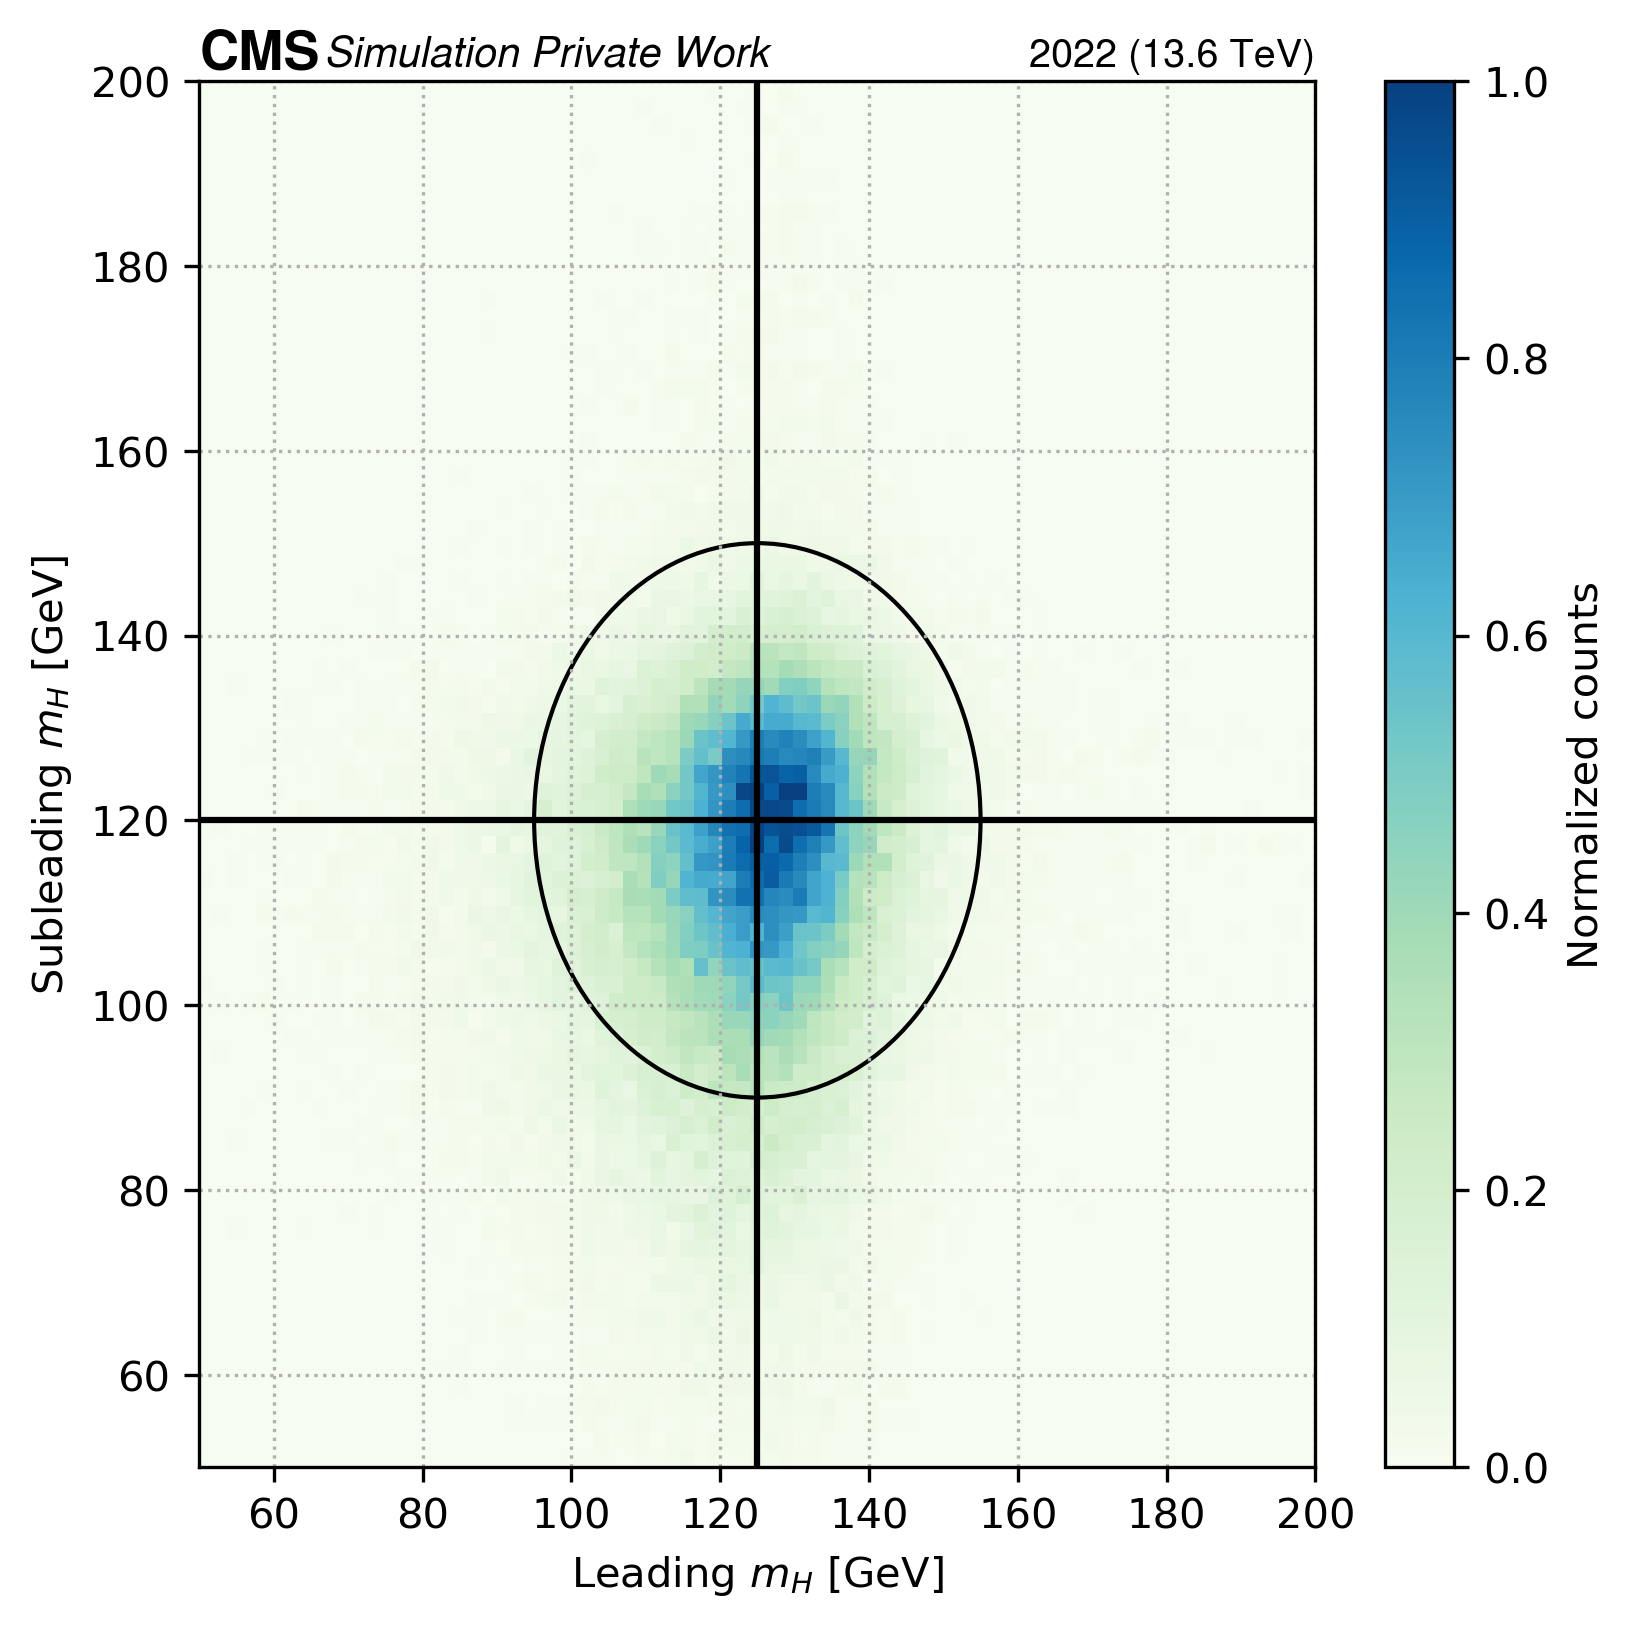
\includegraphics[width=0.6\linewidth]{Images/6.Improving/Mass sculpting/signal mhh.png}
    \caption{2D mass distribution of the evaluation of our model on signal events}
    \label{fig: 2D mass dist sig}
\end{figure}


\begin{figure}[hbt]
    \centering
    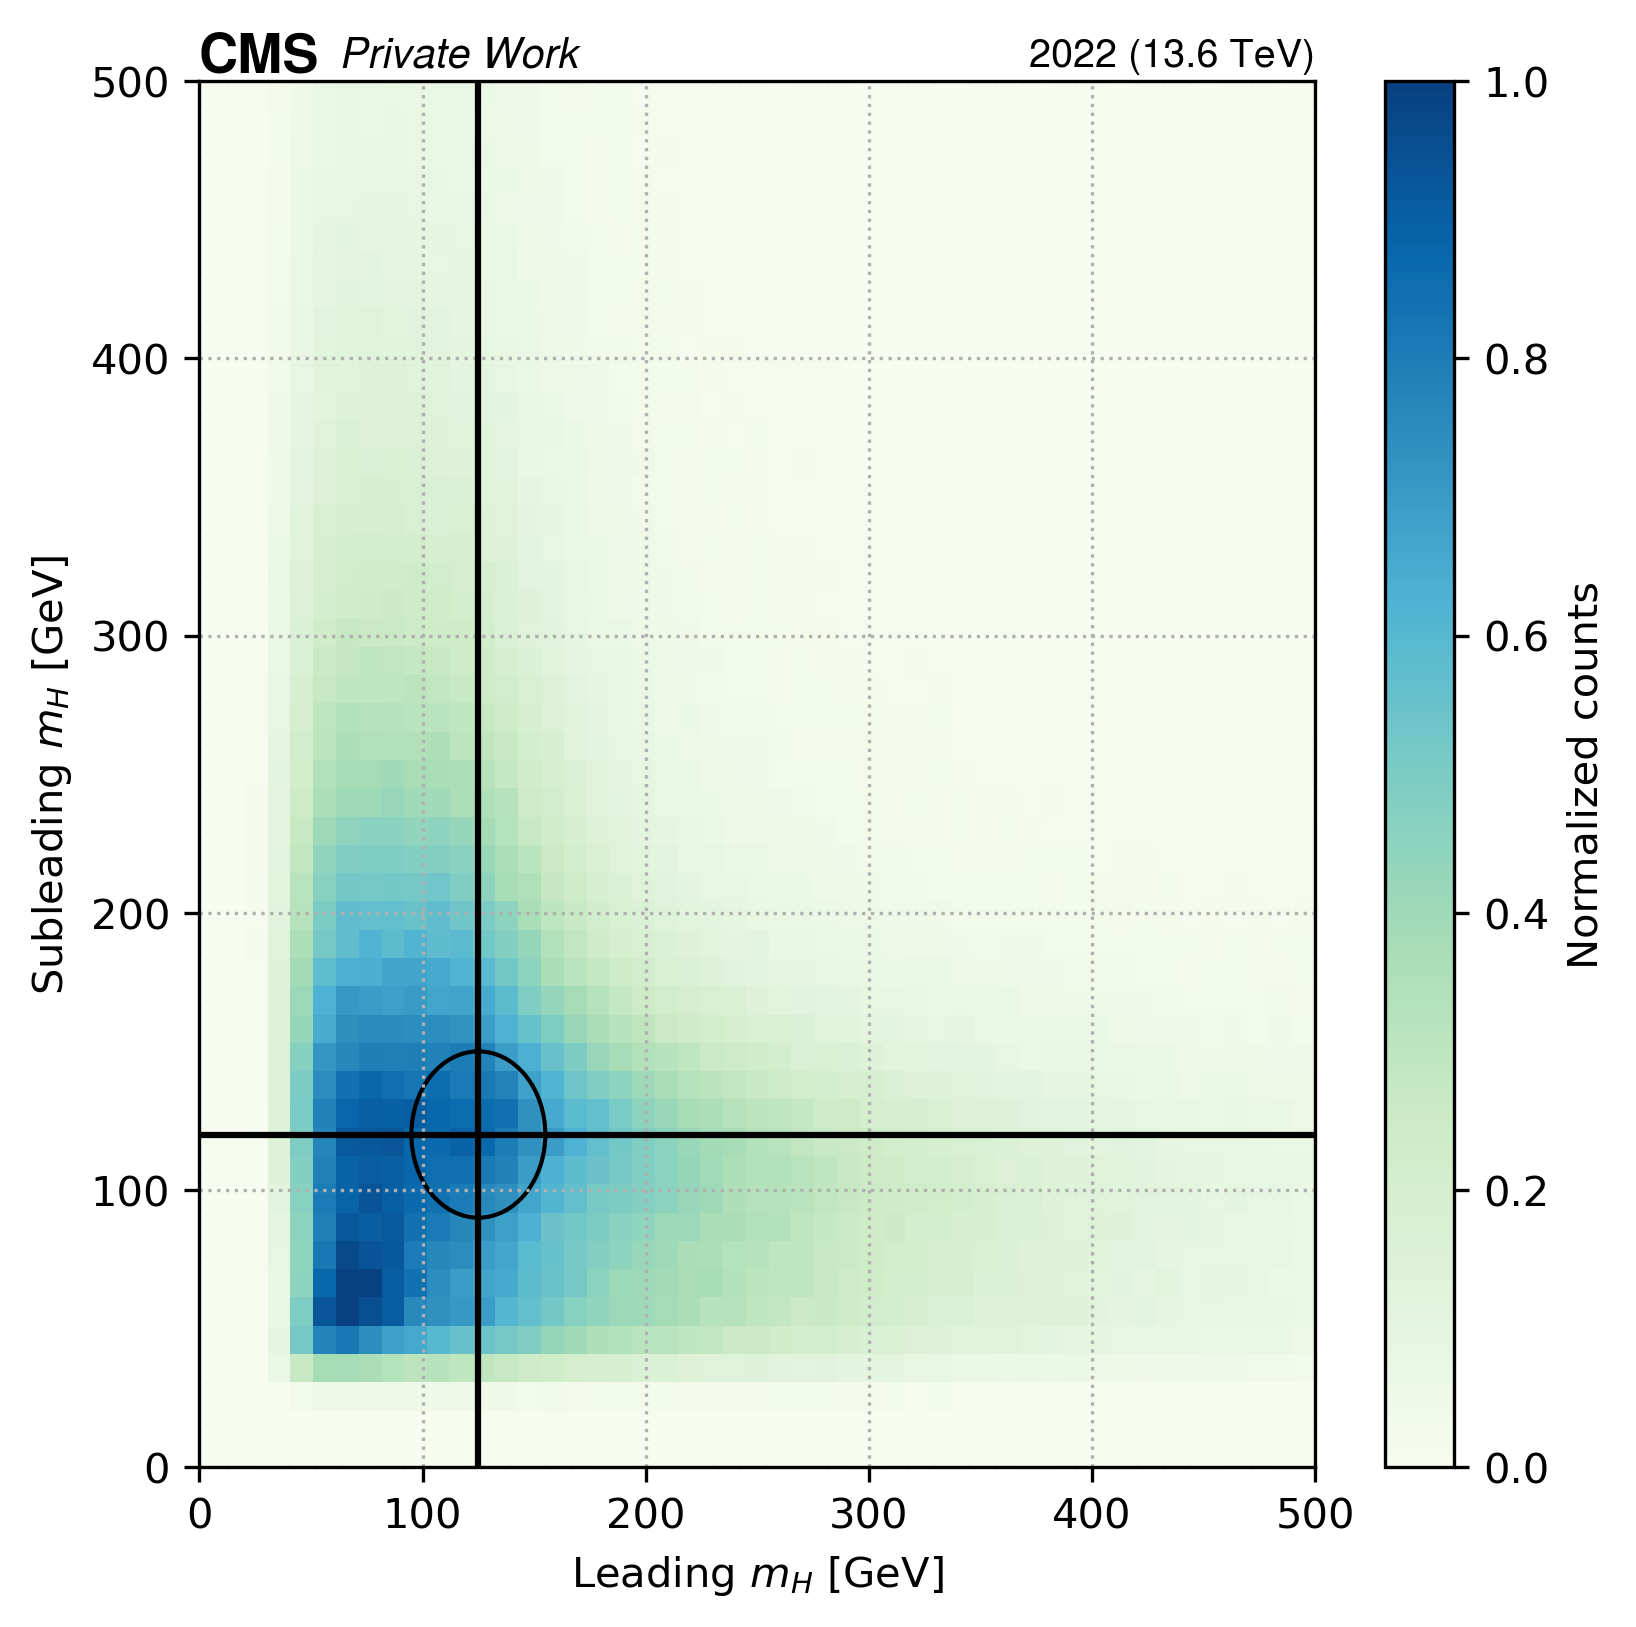
\includegraphics[width=0.6\linewidth]{Images/6.Improving/Mass sculpting/mass sculpting 4j5g.png}
    \caption{2D mass distribution of the evaluation of the 4 jets 5$^{\text{th}}$ jet model on 2b data}
    \label{fig: 2D mass sculpting for 4j5g}
\end{figure}



\begin{figure}[hbt]
    \centering
    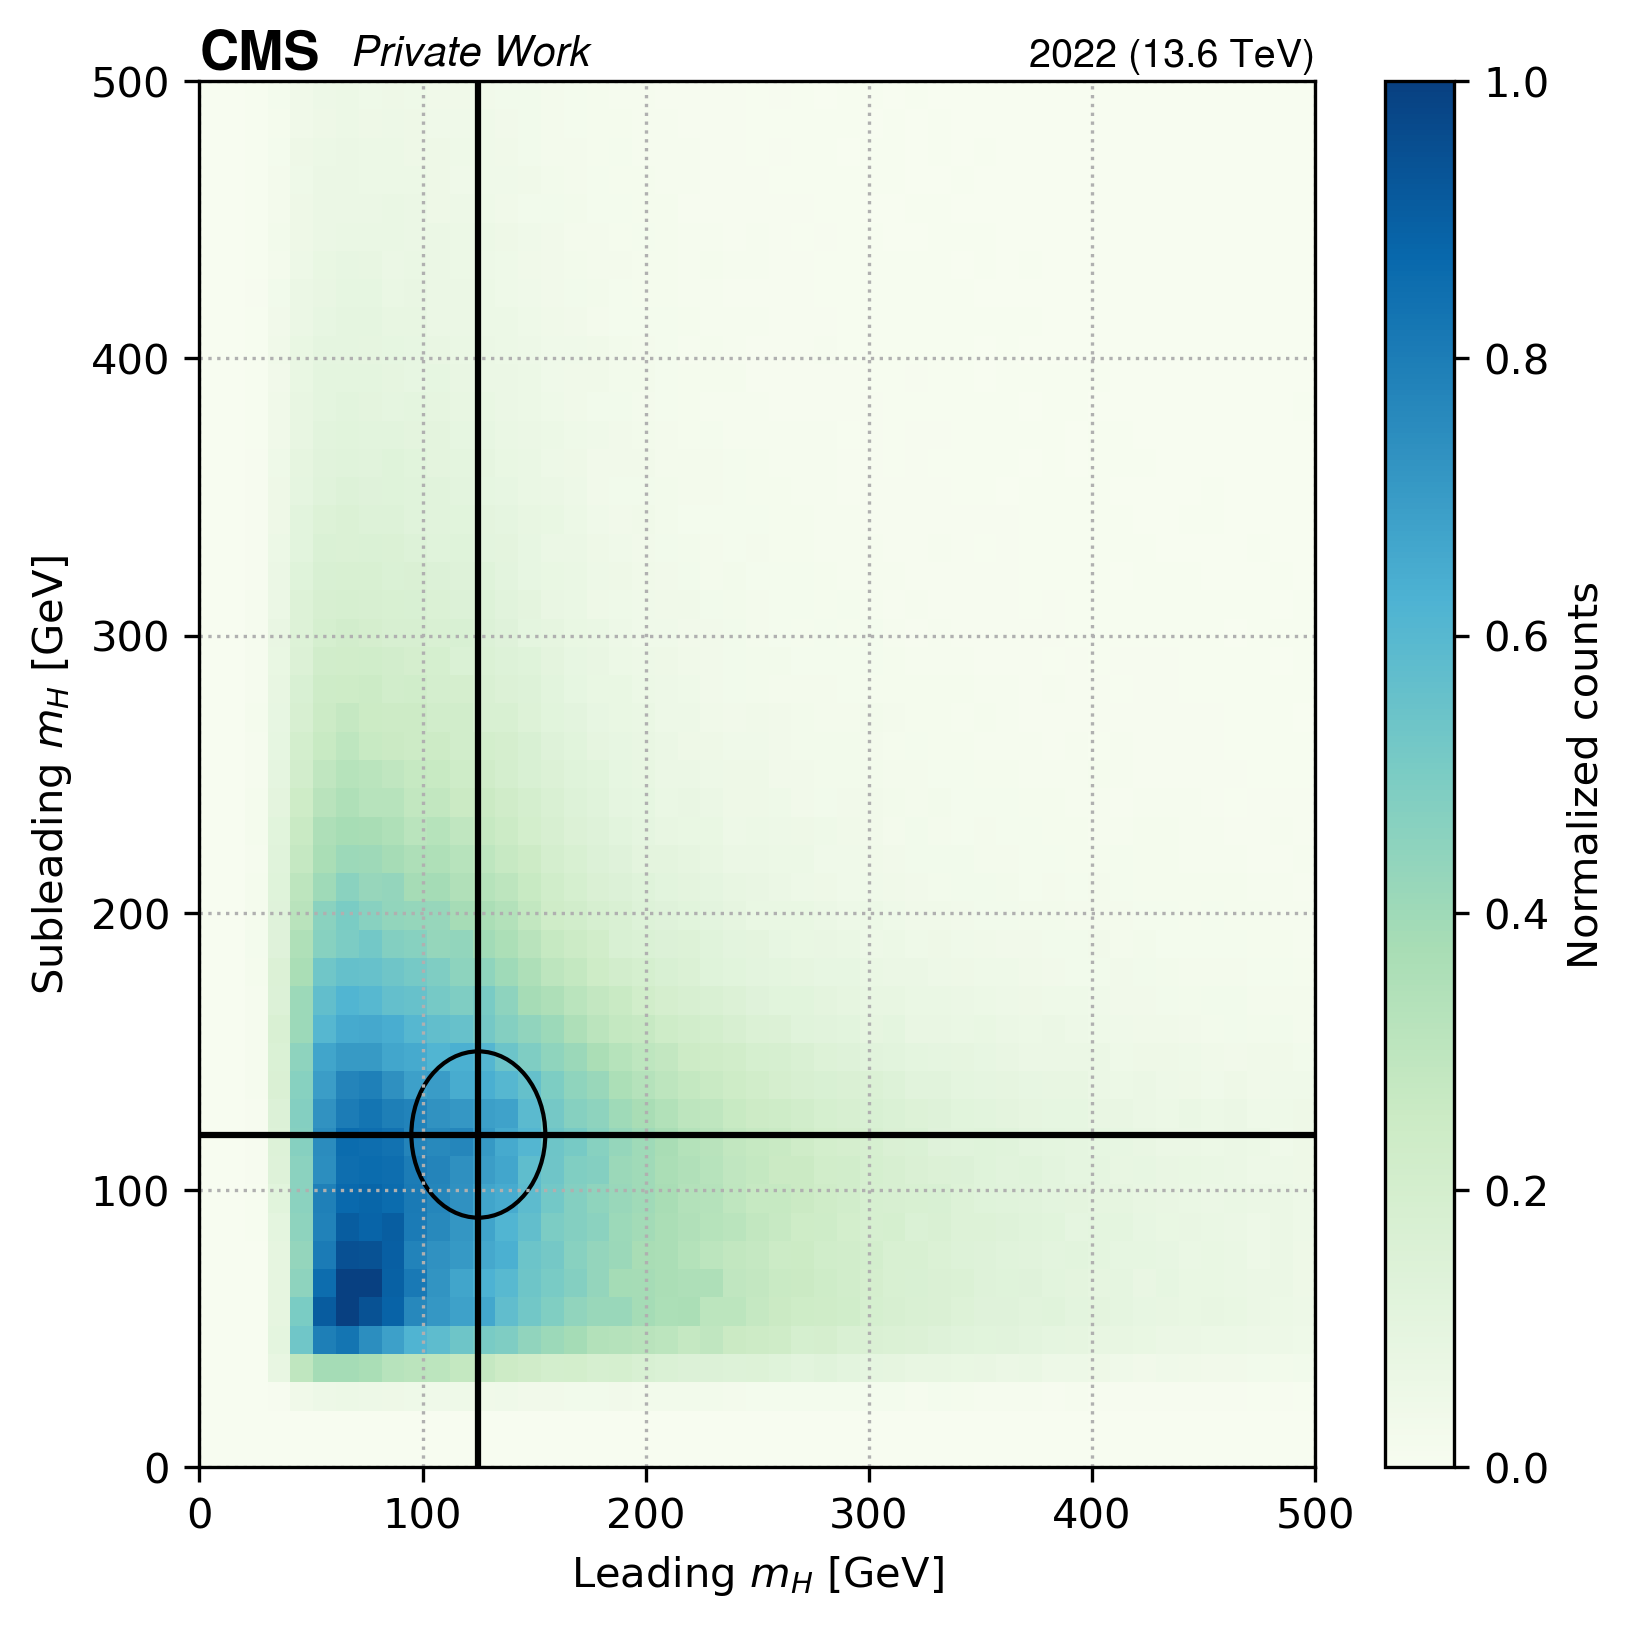
\includegraphics[width=0.6\linewidth]{Images/6.Improving/Mass sculpting/mass sculptimg 5j.png}
    \caption{2D mass distribution of the evaluation of the 5 jet model on 2b data}
    \label{fig: 2D mass sculpting for 5j}
\end{figure}


For more clarity, we can compare these distributions in the 1D plane. These are shown in Figures \ref{fig: 1D mass sculpting leading} and \ref{fig: 1D mass sculpting subleading} for the leading and the subleading Higgs respectively. In these plots we can compare the two models more accurately and conclude that there is less sculpting when considering the training with 5 jets, for both the leading and the subleading Higgs. Therefore, the model where we give 5 jets as inputs, with \pt ref and using the lite hyperparameters not only has the best pairing efficiency but also the mass sculpting is smaller than with the 4 jets model. Therefore, in the following sections, we will use this model.

\begin{figure}[hbt]
    \centering
    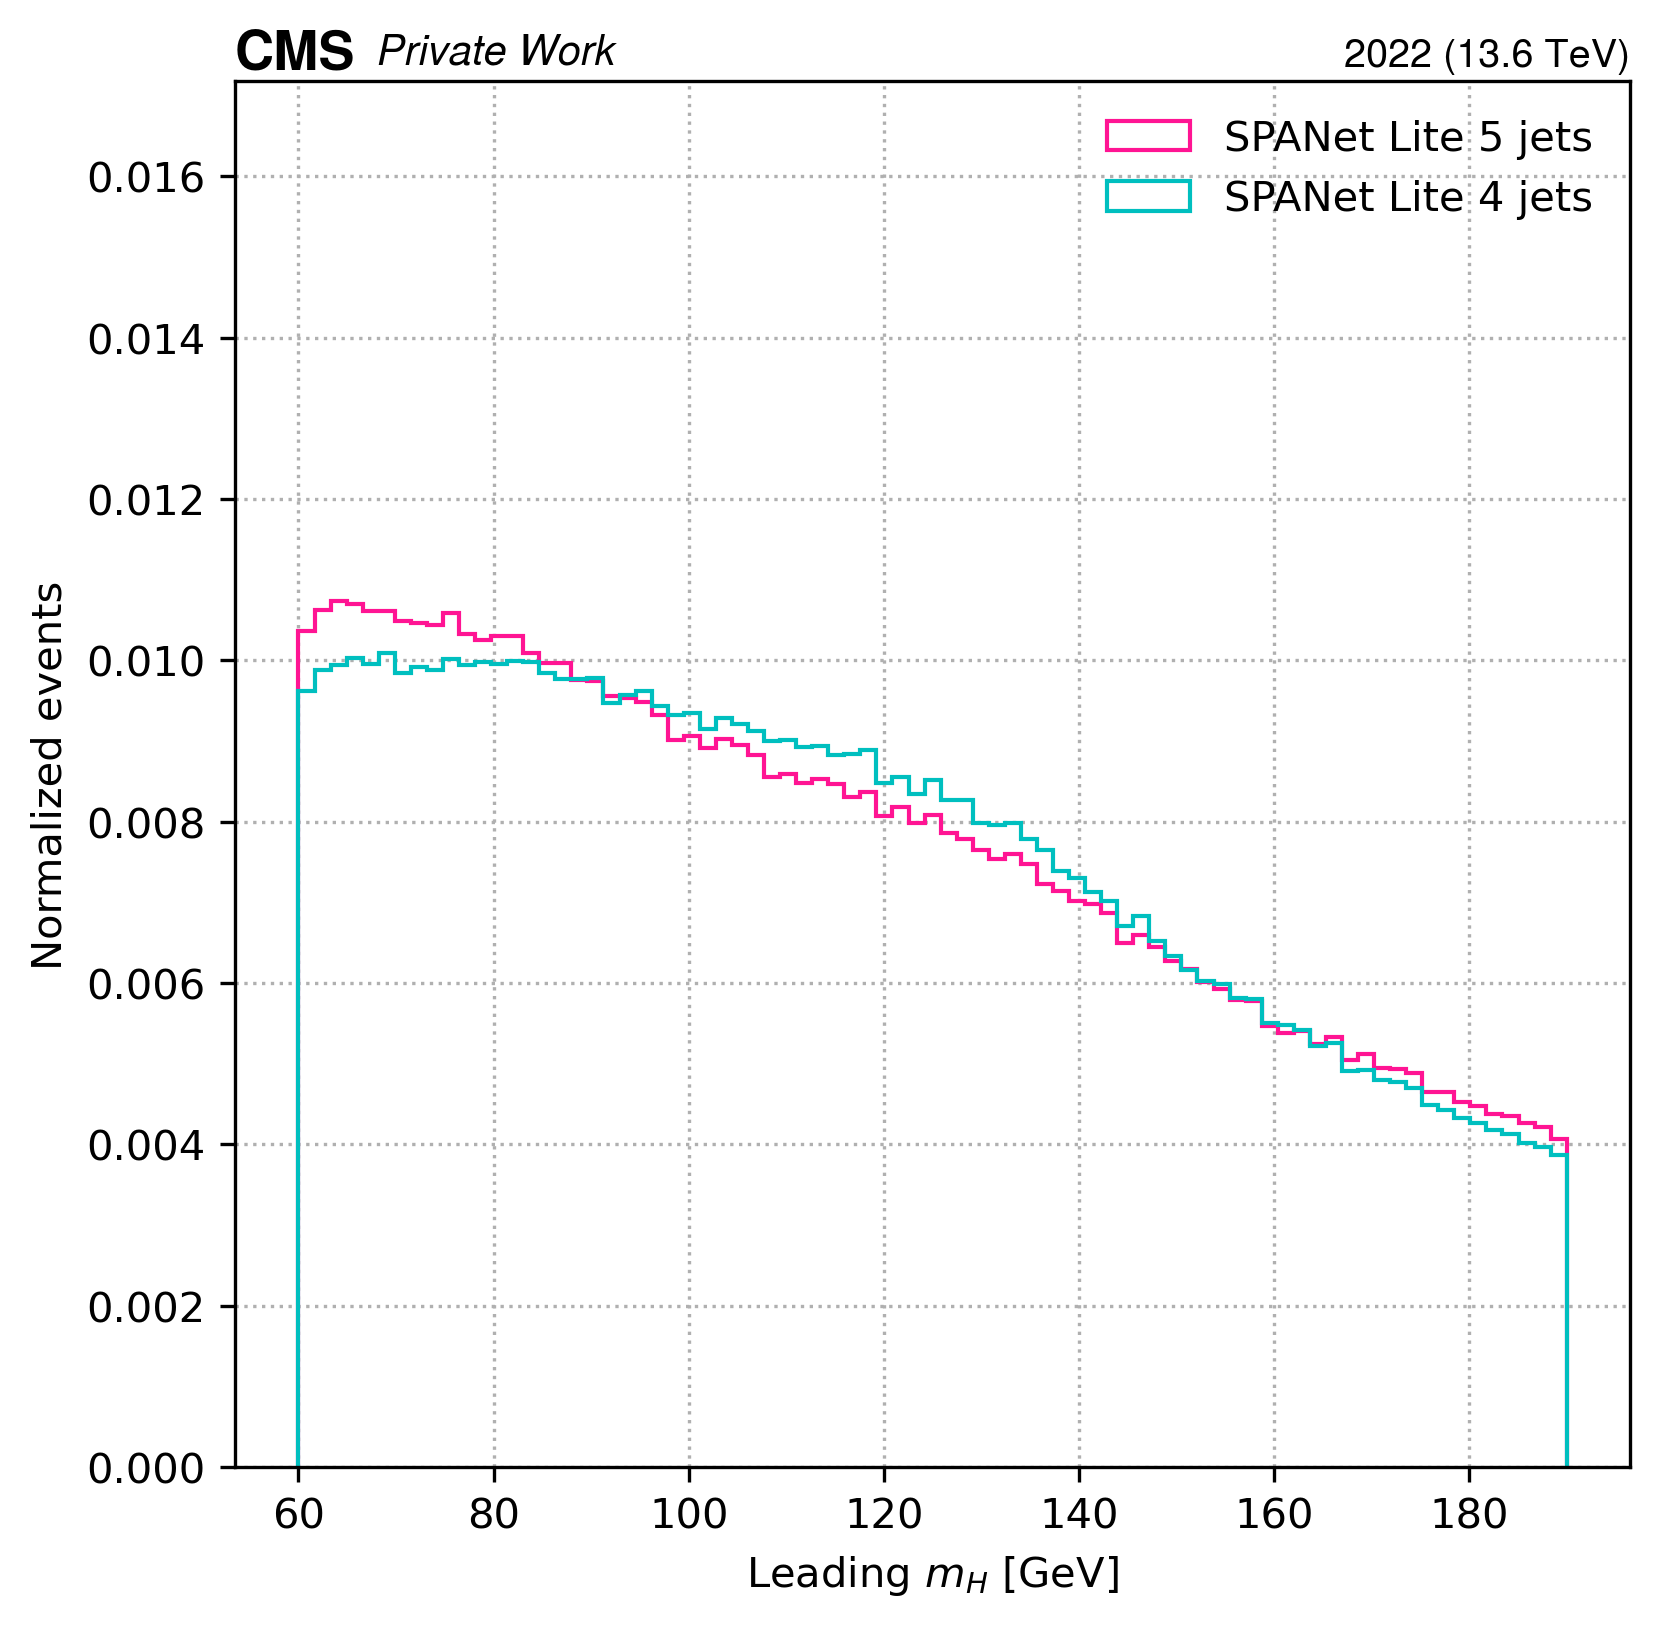
\includegraphics[width=0.6\linewidth]{Images/6.Improving/Mass sculpting/lead h sculpting.png}
    \caption{1D distribution of the Leading Higgs mass for our best models evaluated on 2b data}
    \label{fig: 1D mass sculpting leading}
\end{figure}

\begin{figure}[hbt]
    \centering
    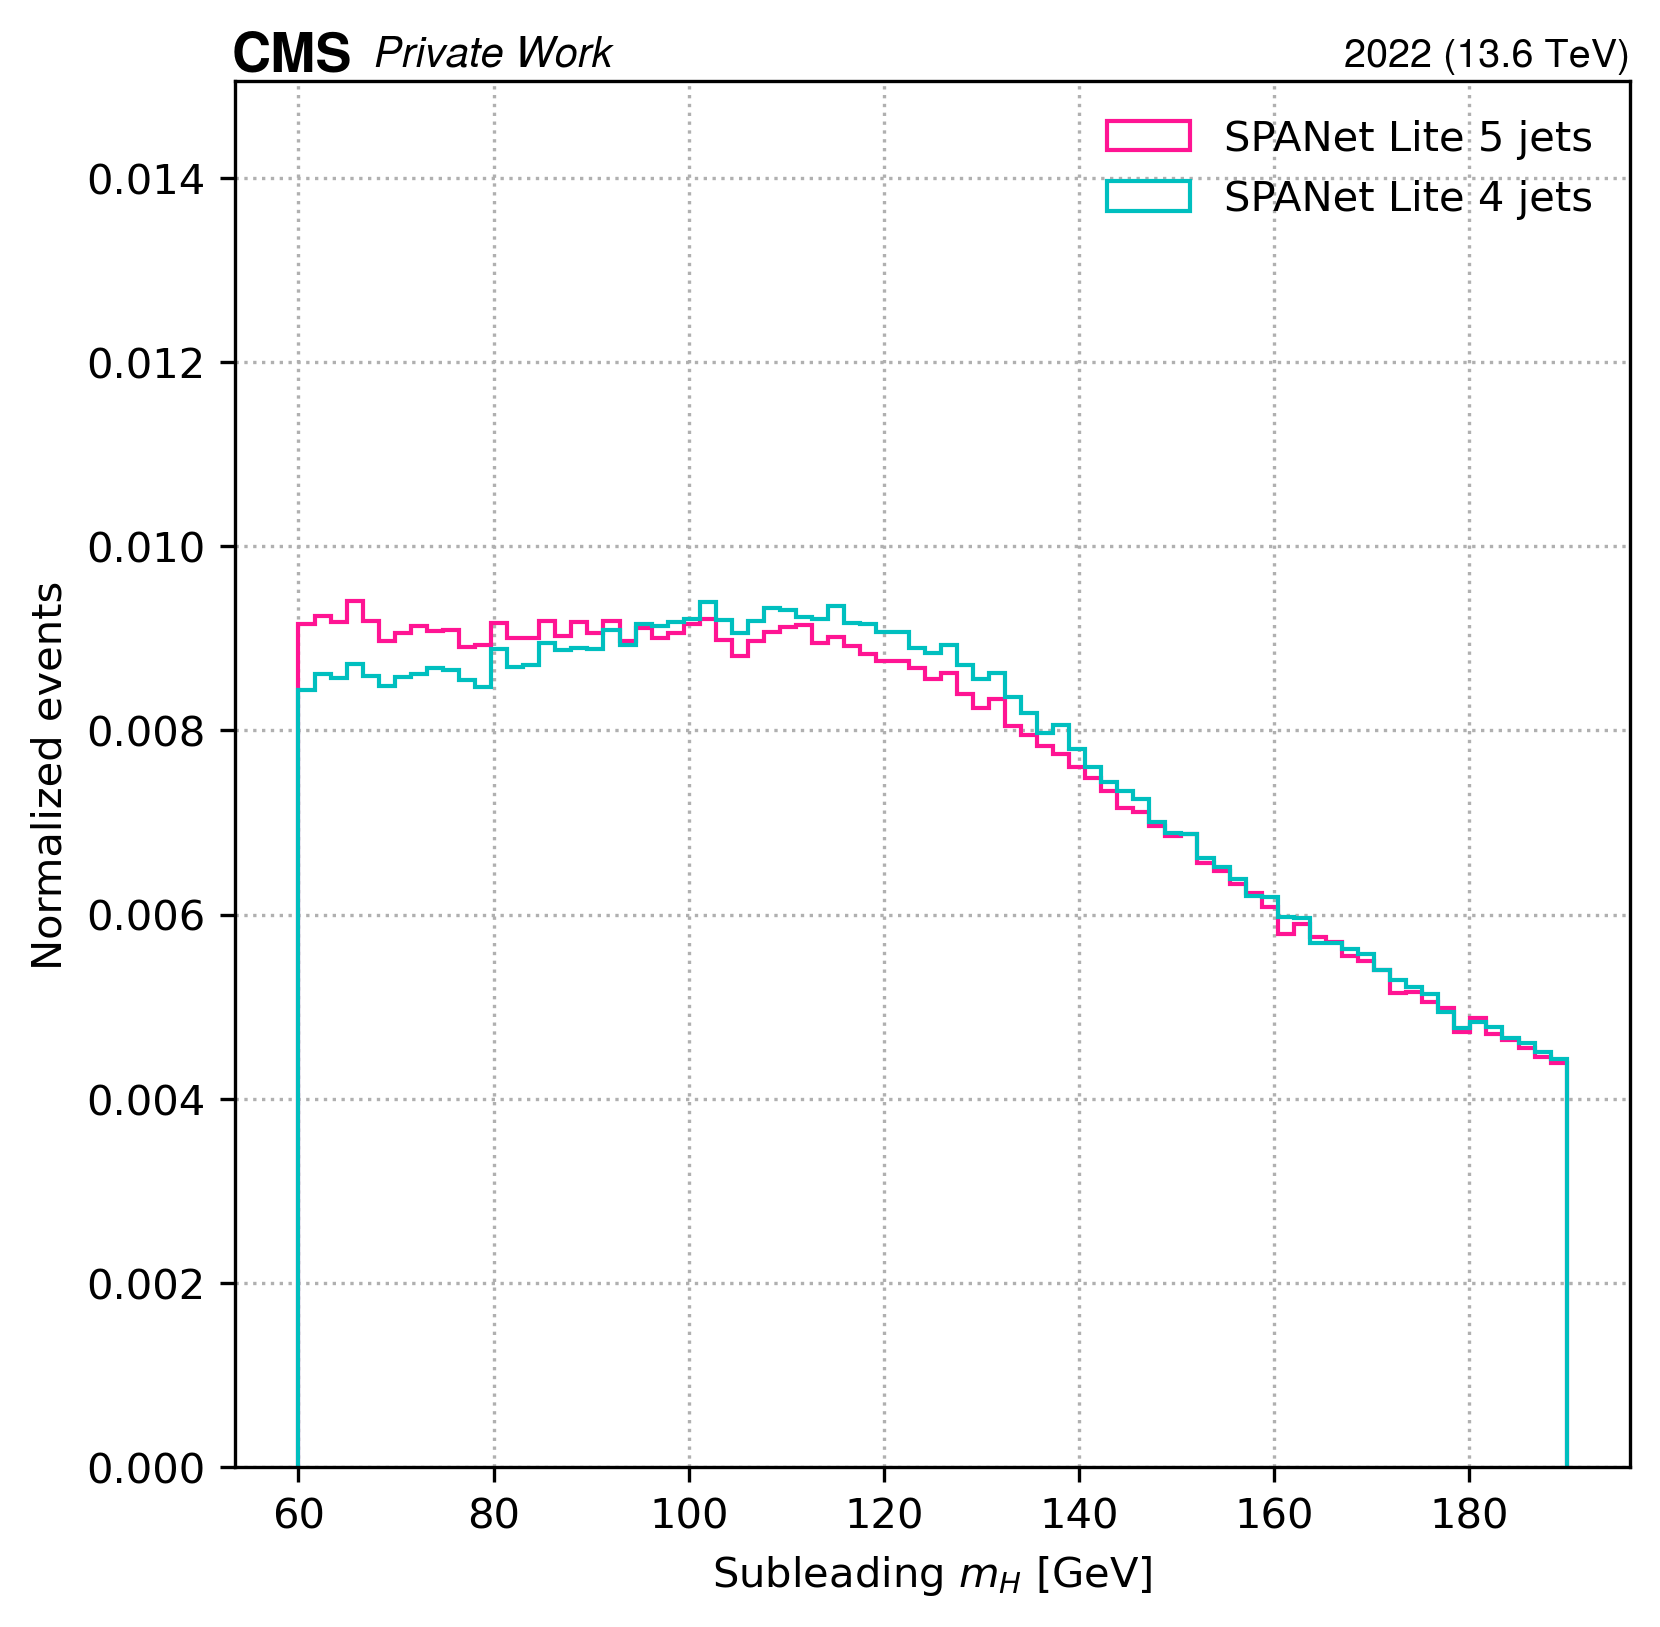
\includegraphics[width=0.6\linewidth]{Images/6.Improving/Mass sculpting/subleading h sculpting.png}
    \caption{1D distribution of the Leading Higgs mass for our best models evaluated on 2b data}
    \label{fig: 1D mass sculpting subleading}
\end{figure}

The next question that arises when performing these tests, is that after performing several trainings with 5 jets, we observed a variability in the results, which is why, we decided to delve onto the variability of these trainings.

\clearpage

\subsection{Studies for the training variability}
So as to asses the variability of our model, we performed several trainings fixing the seed to randomly initialize the weights. As a first test to adress this variability issue, in addition to fixing the weights, we started by verifying if the Pytorch version used for the training had an impact on the variability. To do so, we performed 3 different trainings fixing the seeds to 0, 1 and 2 for 3 different versions of Pytorch. We concluded that the variability is independent of the version we use when we fix the seed to initialize the weights, so we decided to use the latest version (2.2.2) for our future trainings. Then, using this version we performed 26 different trainings with 26 different seeds to observe the variability. The results are shown in Figure \ref{fig: 5j variability}, where we plot the validation accuracy for each training. We can see that it clusters around 2 different values: 96.6\% and 94.5\%. Around each value we have a spread of around 0.3\%. Therefore, with these results we can indeed state that there is a large variability of our model (~2\%), with which we don't outperform the pairing efficiency of Run 2. To solve this this, we aim to modify our hyperparameters in order to stabilize our model.

\begin{figure}[hbt]
    \centering
    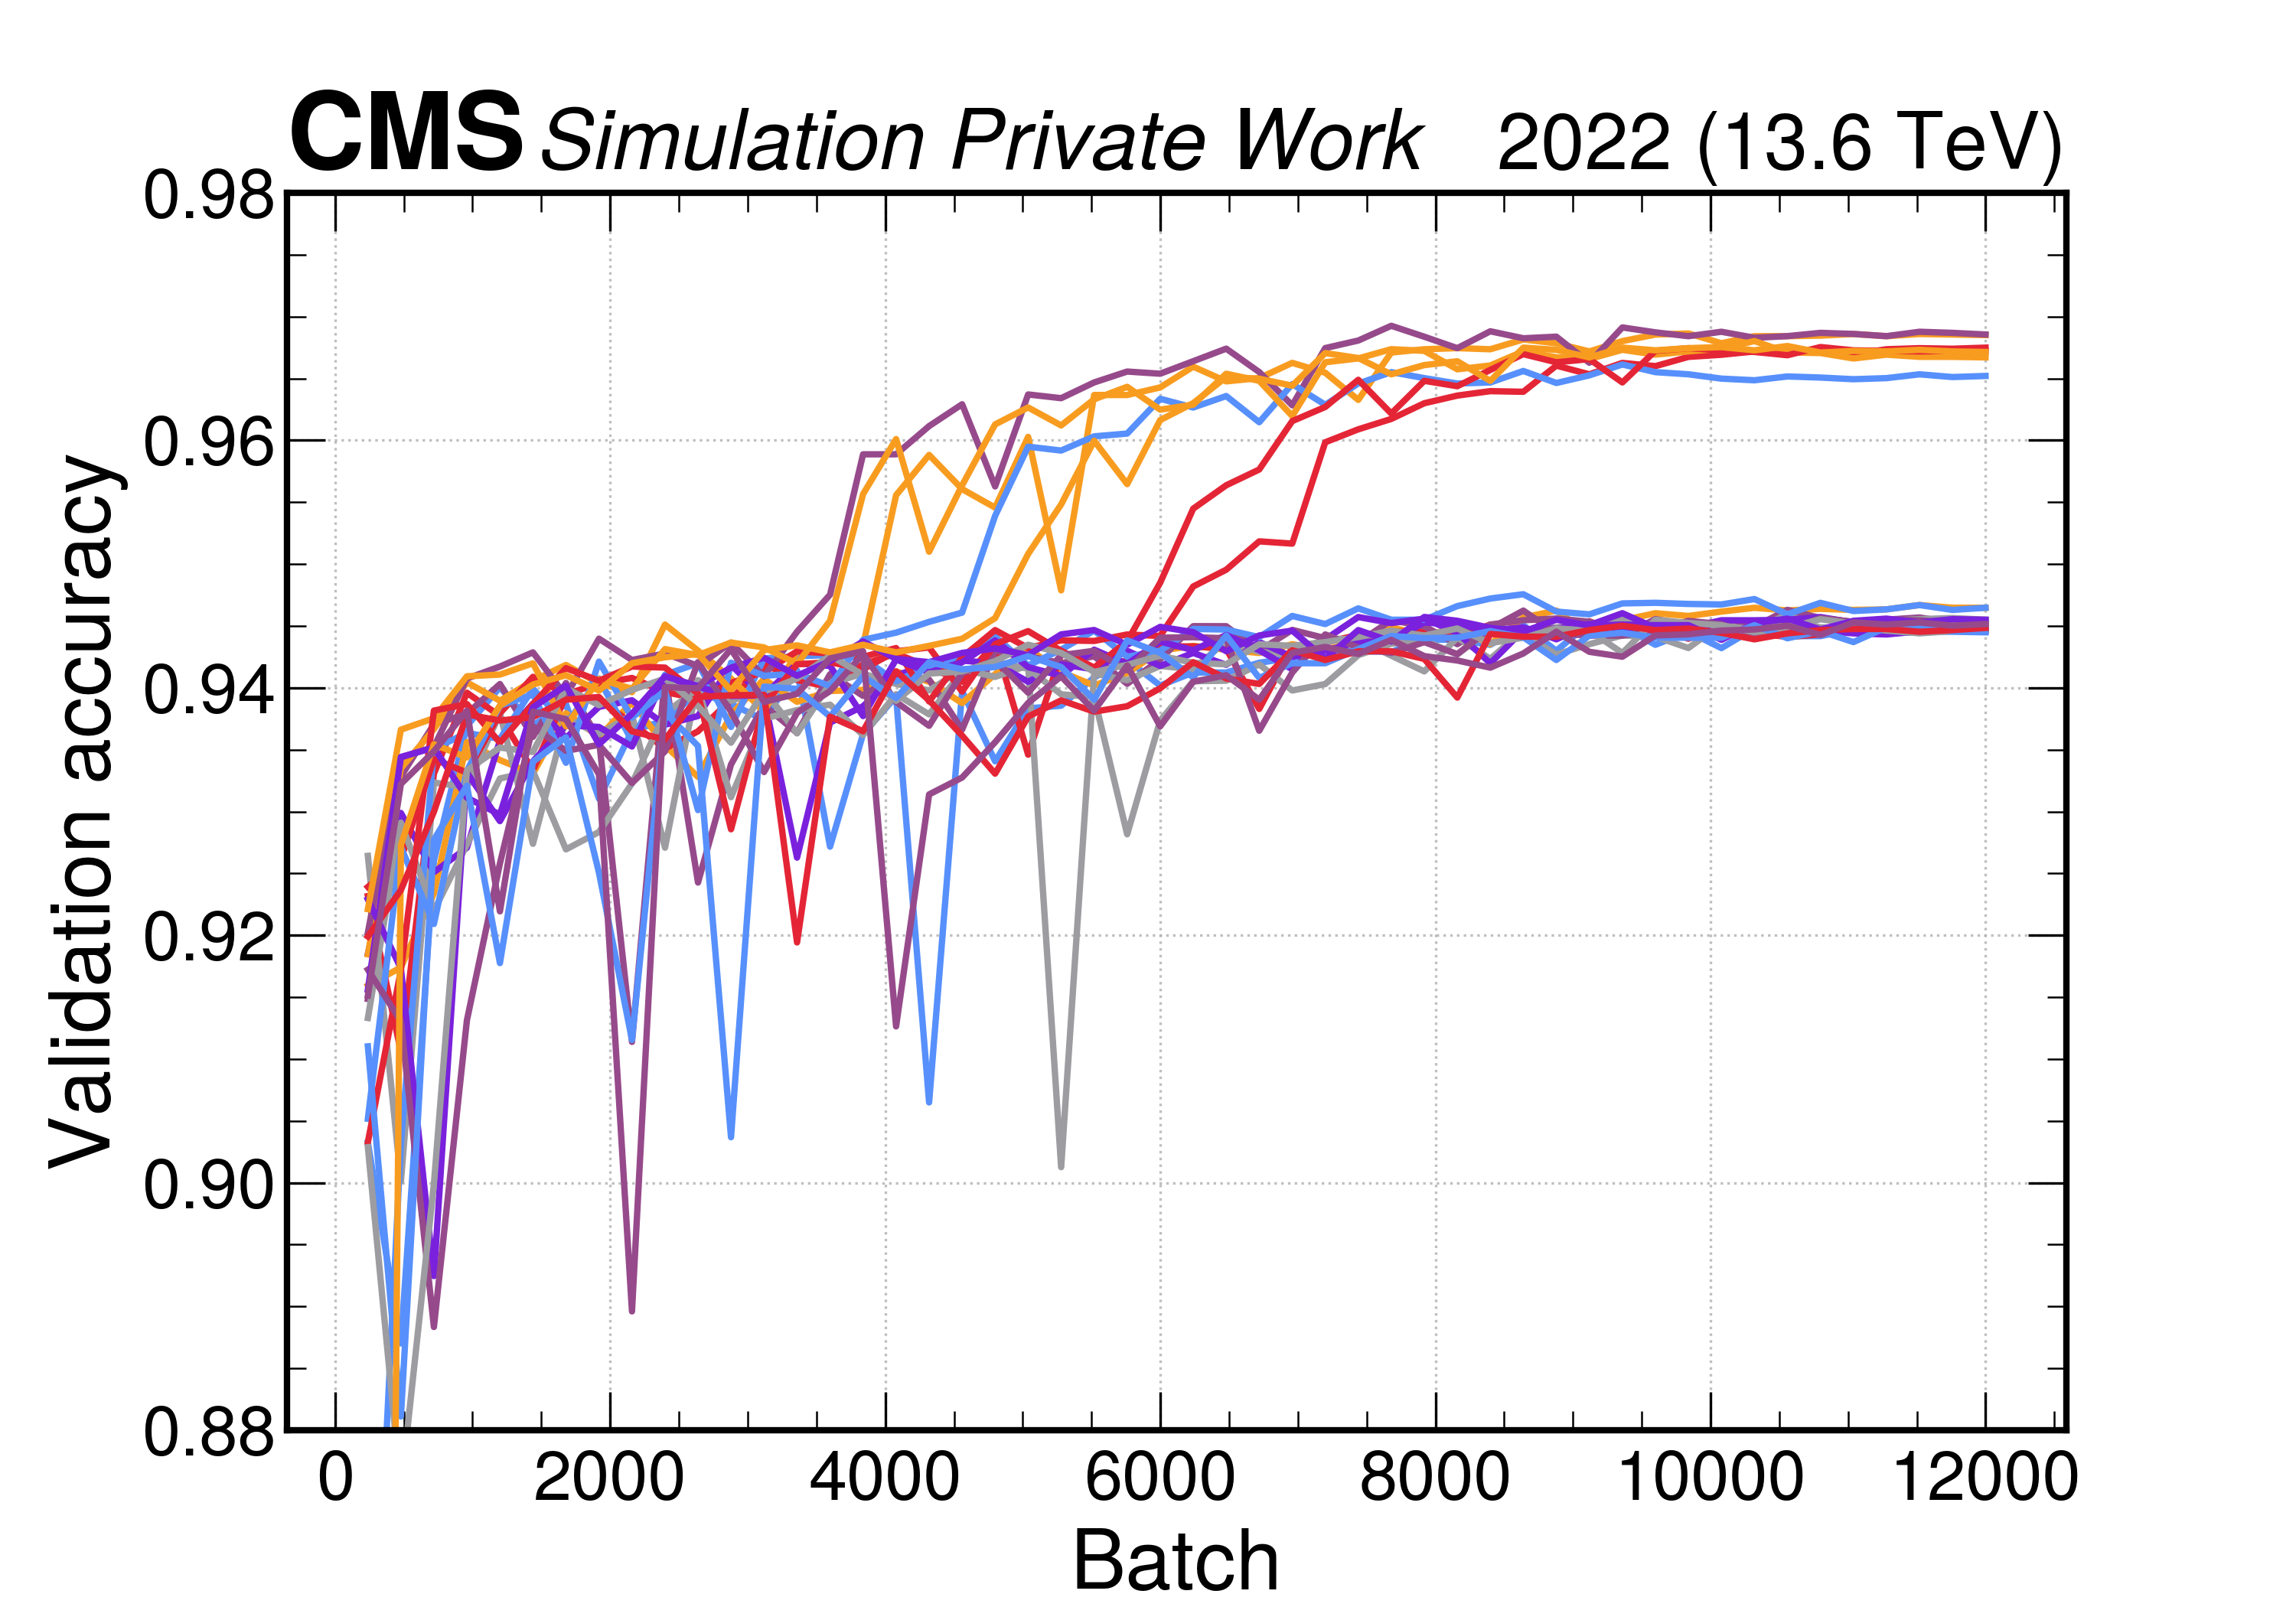
\includegraphics[scale=0.1]{Images/6.Improving/Variability Study/5 jets variability study.png}
    \caption{Variability on the training using 5 jets as inputs \pt reg and lite model parameters}
    \label{fig: 5j variability}
\end{figure}

With the lite model we are using the following hyperparmeters that we aim to modify:

\begin{table}[hbt]
\centering
\begin{tabular}{|p{5cm}|p{4cm}|p{5cm}|}
 \hline
 Hyperparemeters  & Lite model & Test for stabilization \\
 \hline
 Learning rate & 0.00659 & $5\times 10^{-3}$, $10^{-3}$, $5\times 10^{-4}$, $10^{-4}$ \\
 \hline
 Learning rate warmup cycles & 1 & 0\\
 \hline
  Learning rate cycles & 1 & 0\\
 \hline
 Batch size & 2048 / 1024 & 2048/1024 \\
 \hline
 Number of epochs & 50/300 & 50/300 \\
 \hline
\end{tabular}
\caption{Possible variations of the hyperparameters to stabilize the model}
\label{table: }
\end{table}

In figure \ref{fig: lr comp}, we show how the learning rate changes using these new parameters. We can see that instead of reaching the peak of the learning rate after a few epochs, it starts from the maximal value and linearly decreases. After several trainings, we concluded that the most stable configuration is given by the learning rate $10^{-4}$. As we can see in Figure \ref{fig: stable test}, when using the new hyperparameters, taking the smallest learning rate and a batch size of 2048, we see that all of our trainings now cluster around 95.9-96.4\%, which gives a spread of 0.5\%. This variability is acceptable as even taking into account this variability we outperform the Run 2 pairing efficiency. When using a batch size of 1024, our trainings cluster around the same value but with a spread of 0.3\%. However, to use a batch size of 2048 allows us to have faster trainings, therefore, since the difference in the spread is not very significant, we decided to keep a batch size of 2048. 

\begin{figure}[hbt]
    \centering
    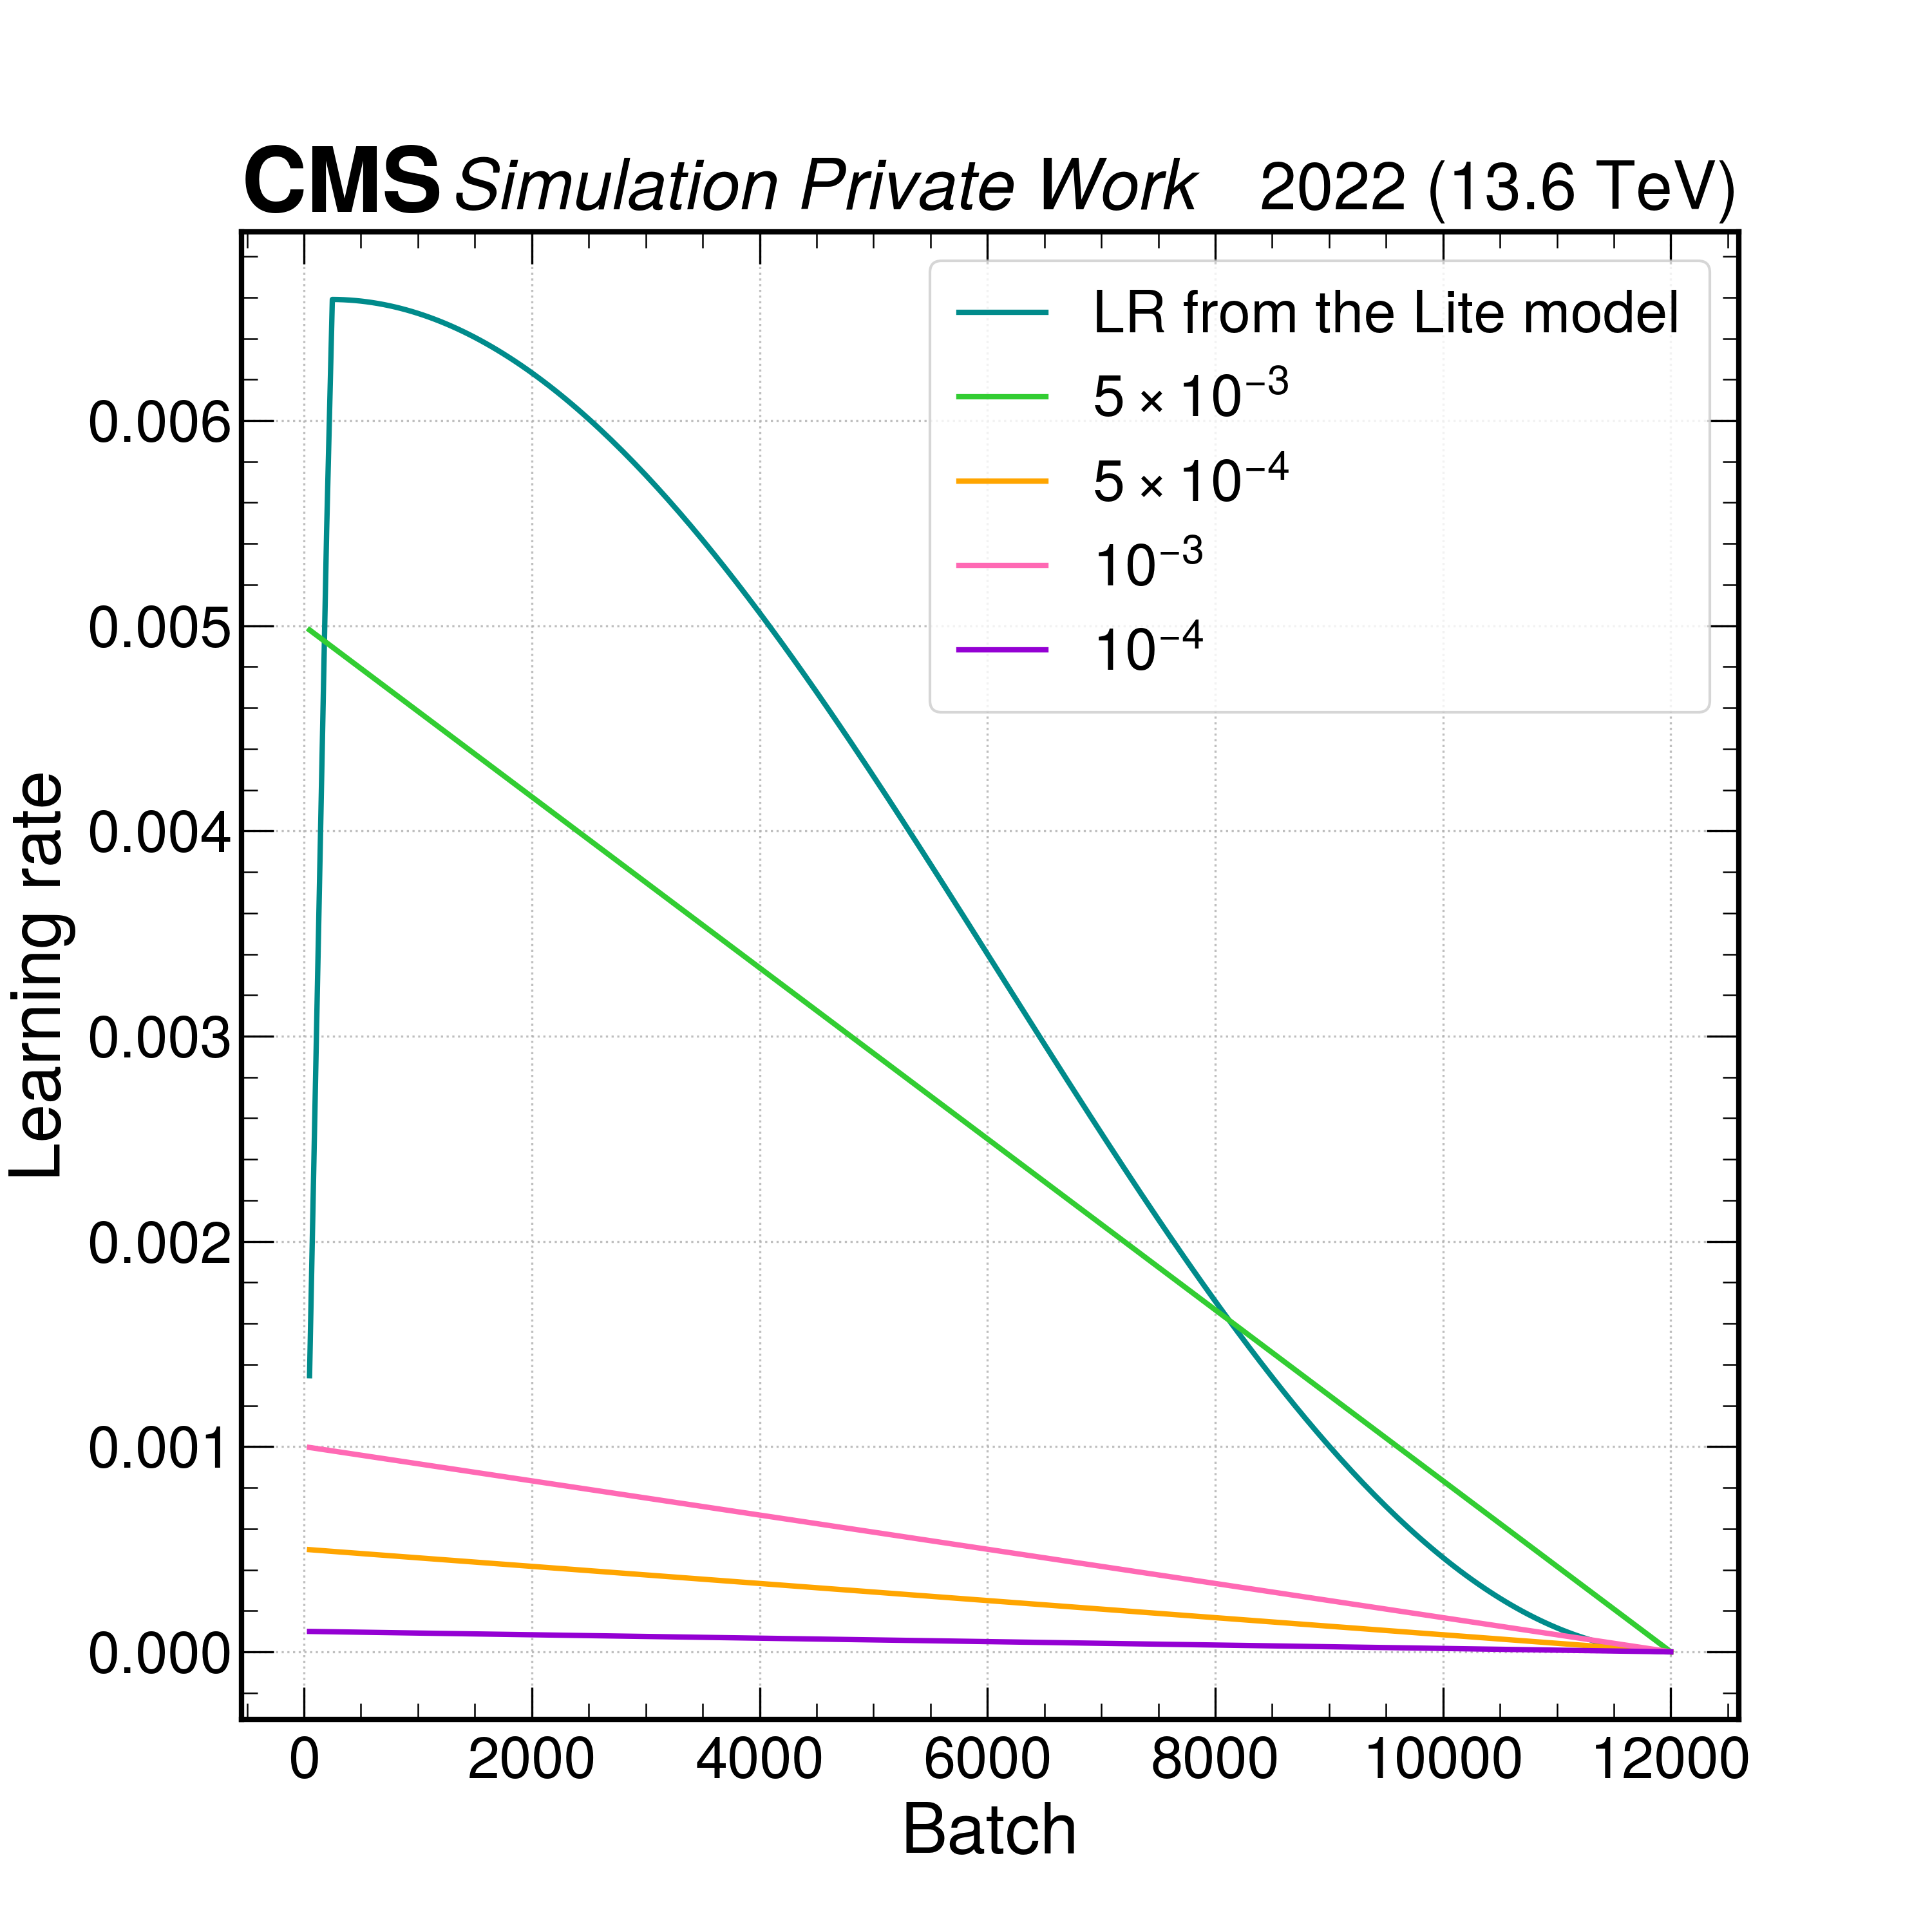
\includegraphics[width=0.6\linewidth]{Images/6.Improving/Variability Study/learning rate comp.png}
    \caption{Comparison of the different learning rates}
    \label{fig: lr comp}
\end{figure}

\begin{figure}[hbt]
    \centering
    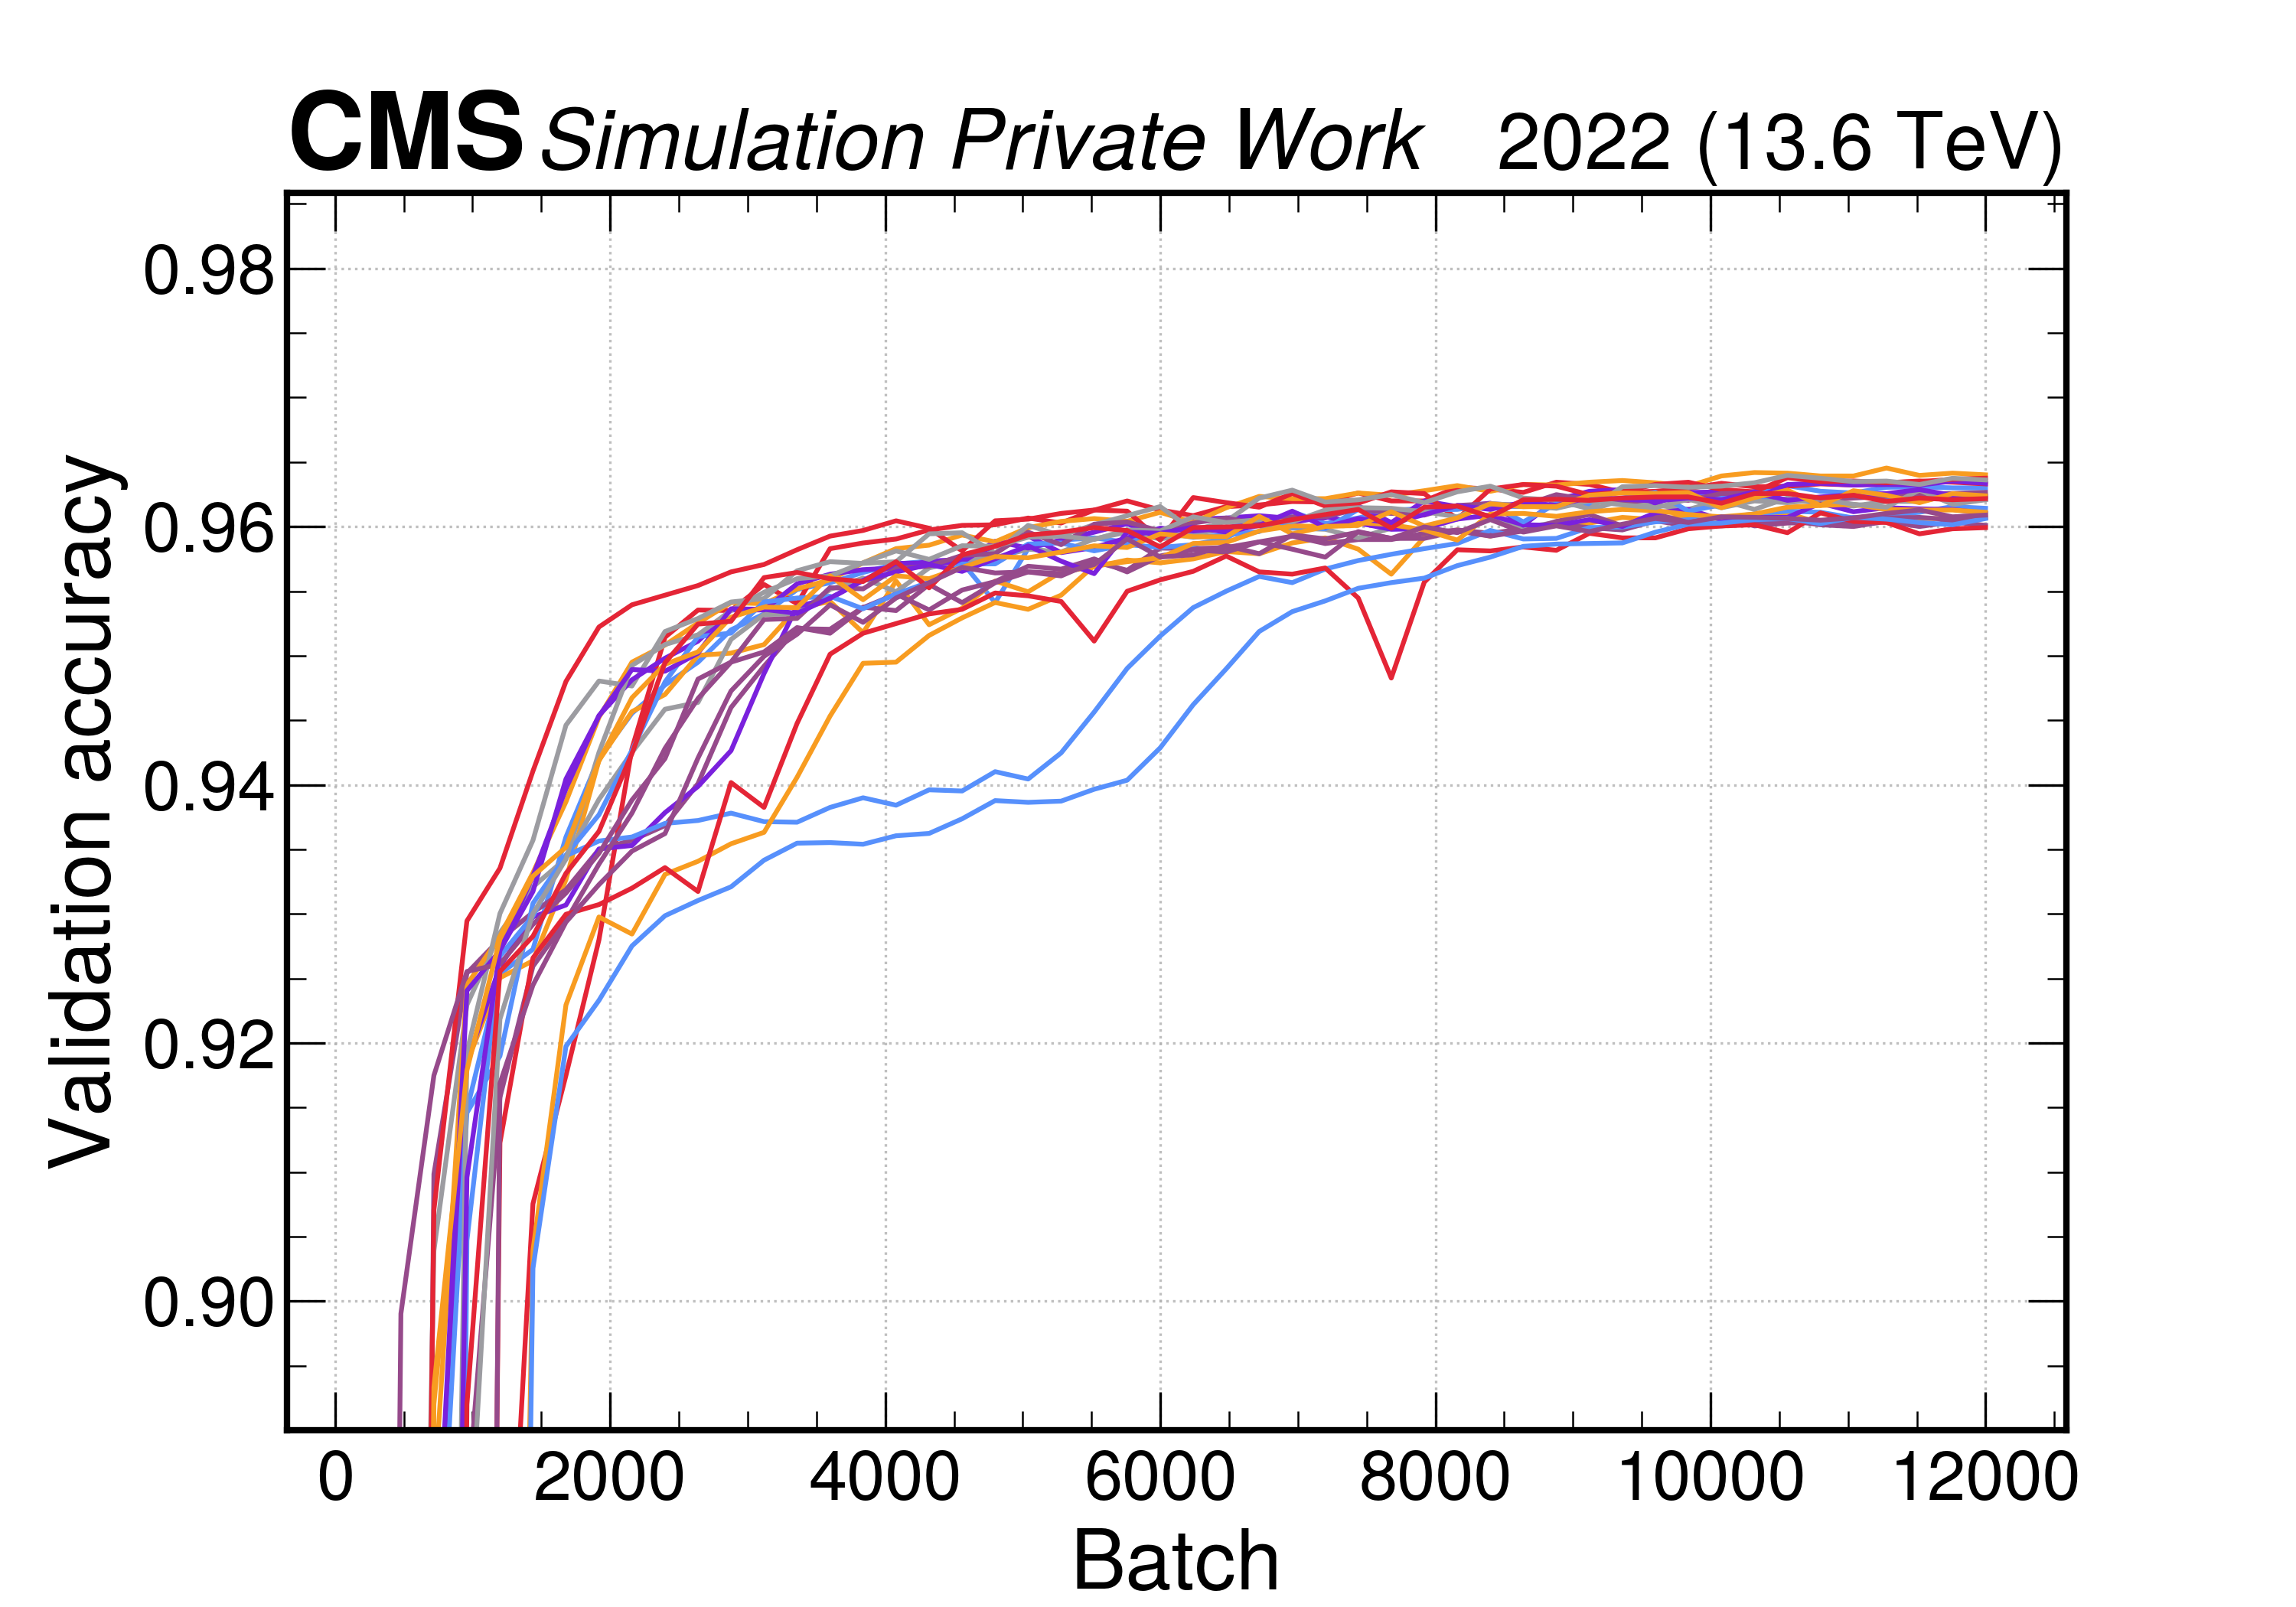
\includegraphics[width=0.7\linewidth]{Images/6.Improving/Variability Study/var 2048.png}
    \caption{Variability on the training using 5 jets as inputs pT reg and stable model parameters from Table \ref{table: stable model}}
    \label{fig: stable test}
\end{figure}

Finally, we studied the difference in the efficiency when varying the number of epochs. In Figure \ref{fig: epoch diff} we can see that is improved by around 0.4\% when using 300 epochs. In conclusion, after this study the most stable and efficient configuration is given by the parameters showed in Table \ref{table: stable model} .

\begin{figure}[hbt]
    \centering
    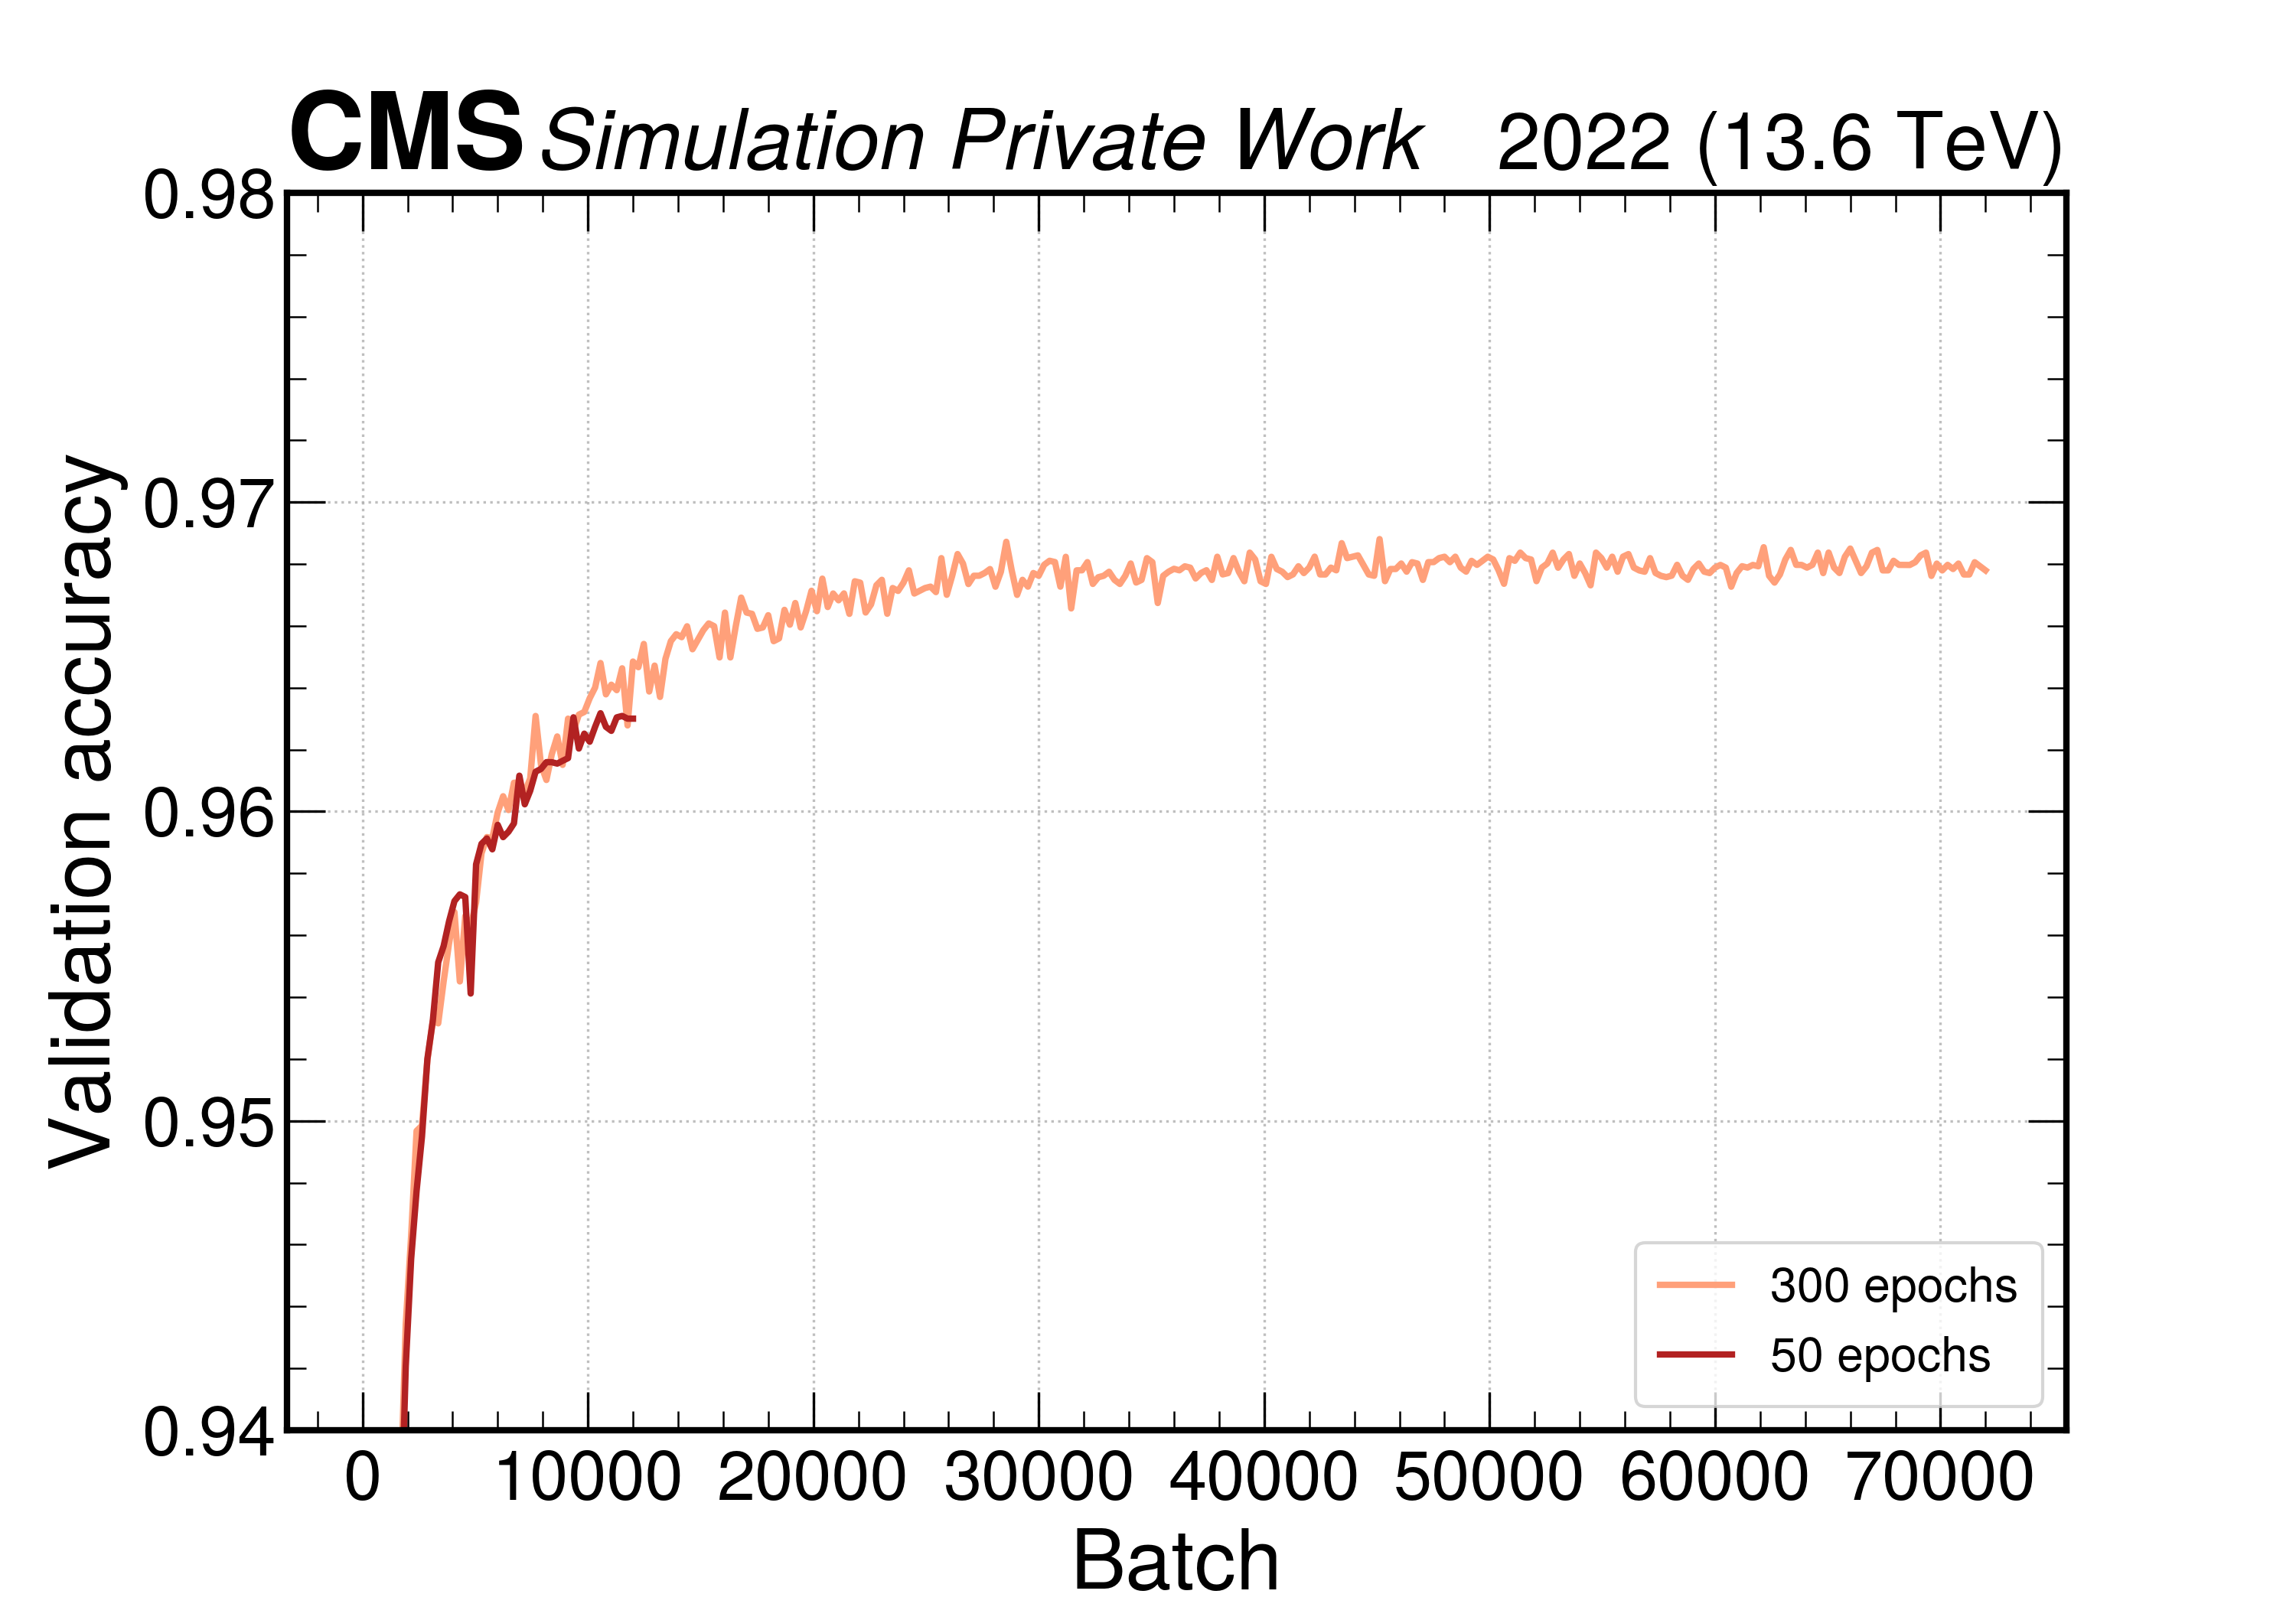
\includegraphics[width=0.7\linewidth]{Images/6.Improving/Variability Study/epoch comp.png}
    \caption{Comparison in the number of epochs of performance the training with 5 jets as inputs using our stable model}
    \label{fig: epoch diff}
\end{figure}

\begin{table}[hbt]
\centering
\begin{tabular}{|c|c|}
 \hline
 Parameters  & Stable model  \\
 \hline
 Learning rate &  $10^{-4}$ \\
 \hline
 Learning rate warmup cycles &  0\\
 \hline
  Learning rate cycles & 0\\
 \hline
 Batch size & 2048 \\
 \hline
 Number of epochs & 300 \\
 \hline
\end{tabular}
\caption{Configuration for the Stable model}
\label{table: stable model}
\end{table}


We will stick to this configuration for our model in the following sections. As a last test to increase the performance of our model, we perform a grid search, thank to which we are able to tune some of our parameters. This will be presented in the following section.

\newpage

\subsection{Grid search}
To increase the pairing efficiency, we performed a grid search in order to tune some of the parameters. 
To do so, we used the features of the Stable model and changed the hyperparameters presented in Table \ref{table: parameters for the grid search}. 
However, contrary to what is specified in Table \ref{table: stable model} for this grid search we will use 50 epochs given the limited resources at our disposal.
As can be seen in Table \ref{table: parameters for the grid search}, we give different possible values for the hyperparameters and then we perform several tests combining them differently.
In particular for the first 3, we need to choose between the ones specifies, whereas for the L2 Penalty we can continually (in log scale) choose a value between [1e-5 : 1e-3].
The final output of this search will be the combination of hyperparameters that give the best performance which are shown in Table \ref{table: grid search}.


\begin{table}[hbt]
   \centering
   \begin{tabular}{|c|c|}
    \hline
    Hidden dimension  &  \{32, 64, 96\}  \\
    \hline
   Number of encoder layers & \{5, 6, 7, 8\} \\
    \hline
    Number of branch embedding layers &  \{1, 2, 3, 4\}\\
    \hline
     Number of branch encoder layers & 4\\
    \hline
    Number of regression layers & 3 \\
    \hline
    Number of classification layers & 1 \\
    \hline
    Focal gamma & 0.0 \\
    \hline
    L2 Penalty & [1e-5 : 1e-3] \\
    \hline
   \end{tabular}
   \caption{Final hyperparameters determined by the grid search}
   \label{table: parameters for the grid search}
   \end{table}



\begin{table}[hbt]
\centering
\begin{tabular}{|c|c|}
 \hline
 Hidden dimension  &  96  \\
 \hline
Number of encoder layers & 5 \\
 \hline
 Number of branch embedding layers &  3\\
 \hline
  Number of branch encoder layers & 4\\
 \hline
 Number of regression layers & 3 \\
 \hline
 Number of classification layers & 1 \\
 \hline
 Focal gamma & 0.0 \\
 \hline
 L2 Penalty & $7.3\times 10^{-4}$ \\
 \hline
\end{tabular}
\caption{Final hyperparameters determined by the grid search}
\label{table: grid search}
\end{table}

By using these new hyperparameters our model has 5.1 M trainable parameters compared to 0.5 M in the Stable model. 
As can be seen in Figure \ref{fig: comp grid search}, by using this new hyperparameters, with which we have a much larger model, 
we don't increase that much the performance compared to the Stable model performance. 
Hence, we decided to use the hyperparameters from the Stable Model since it's lighter and the trainings take less time.

\begin{figure}[hbt]
    \centering
    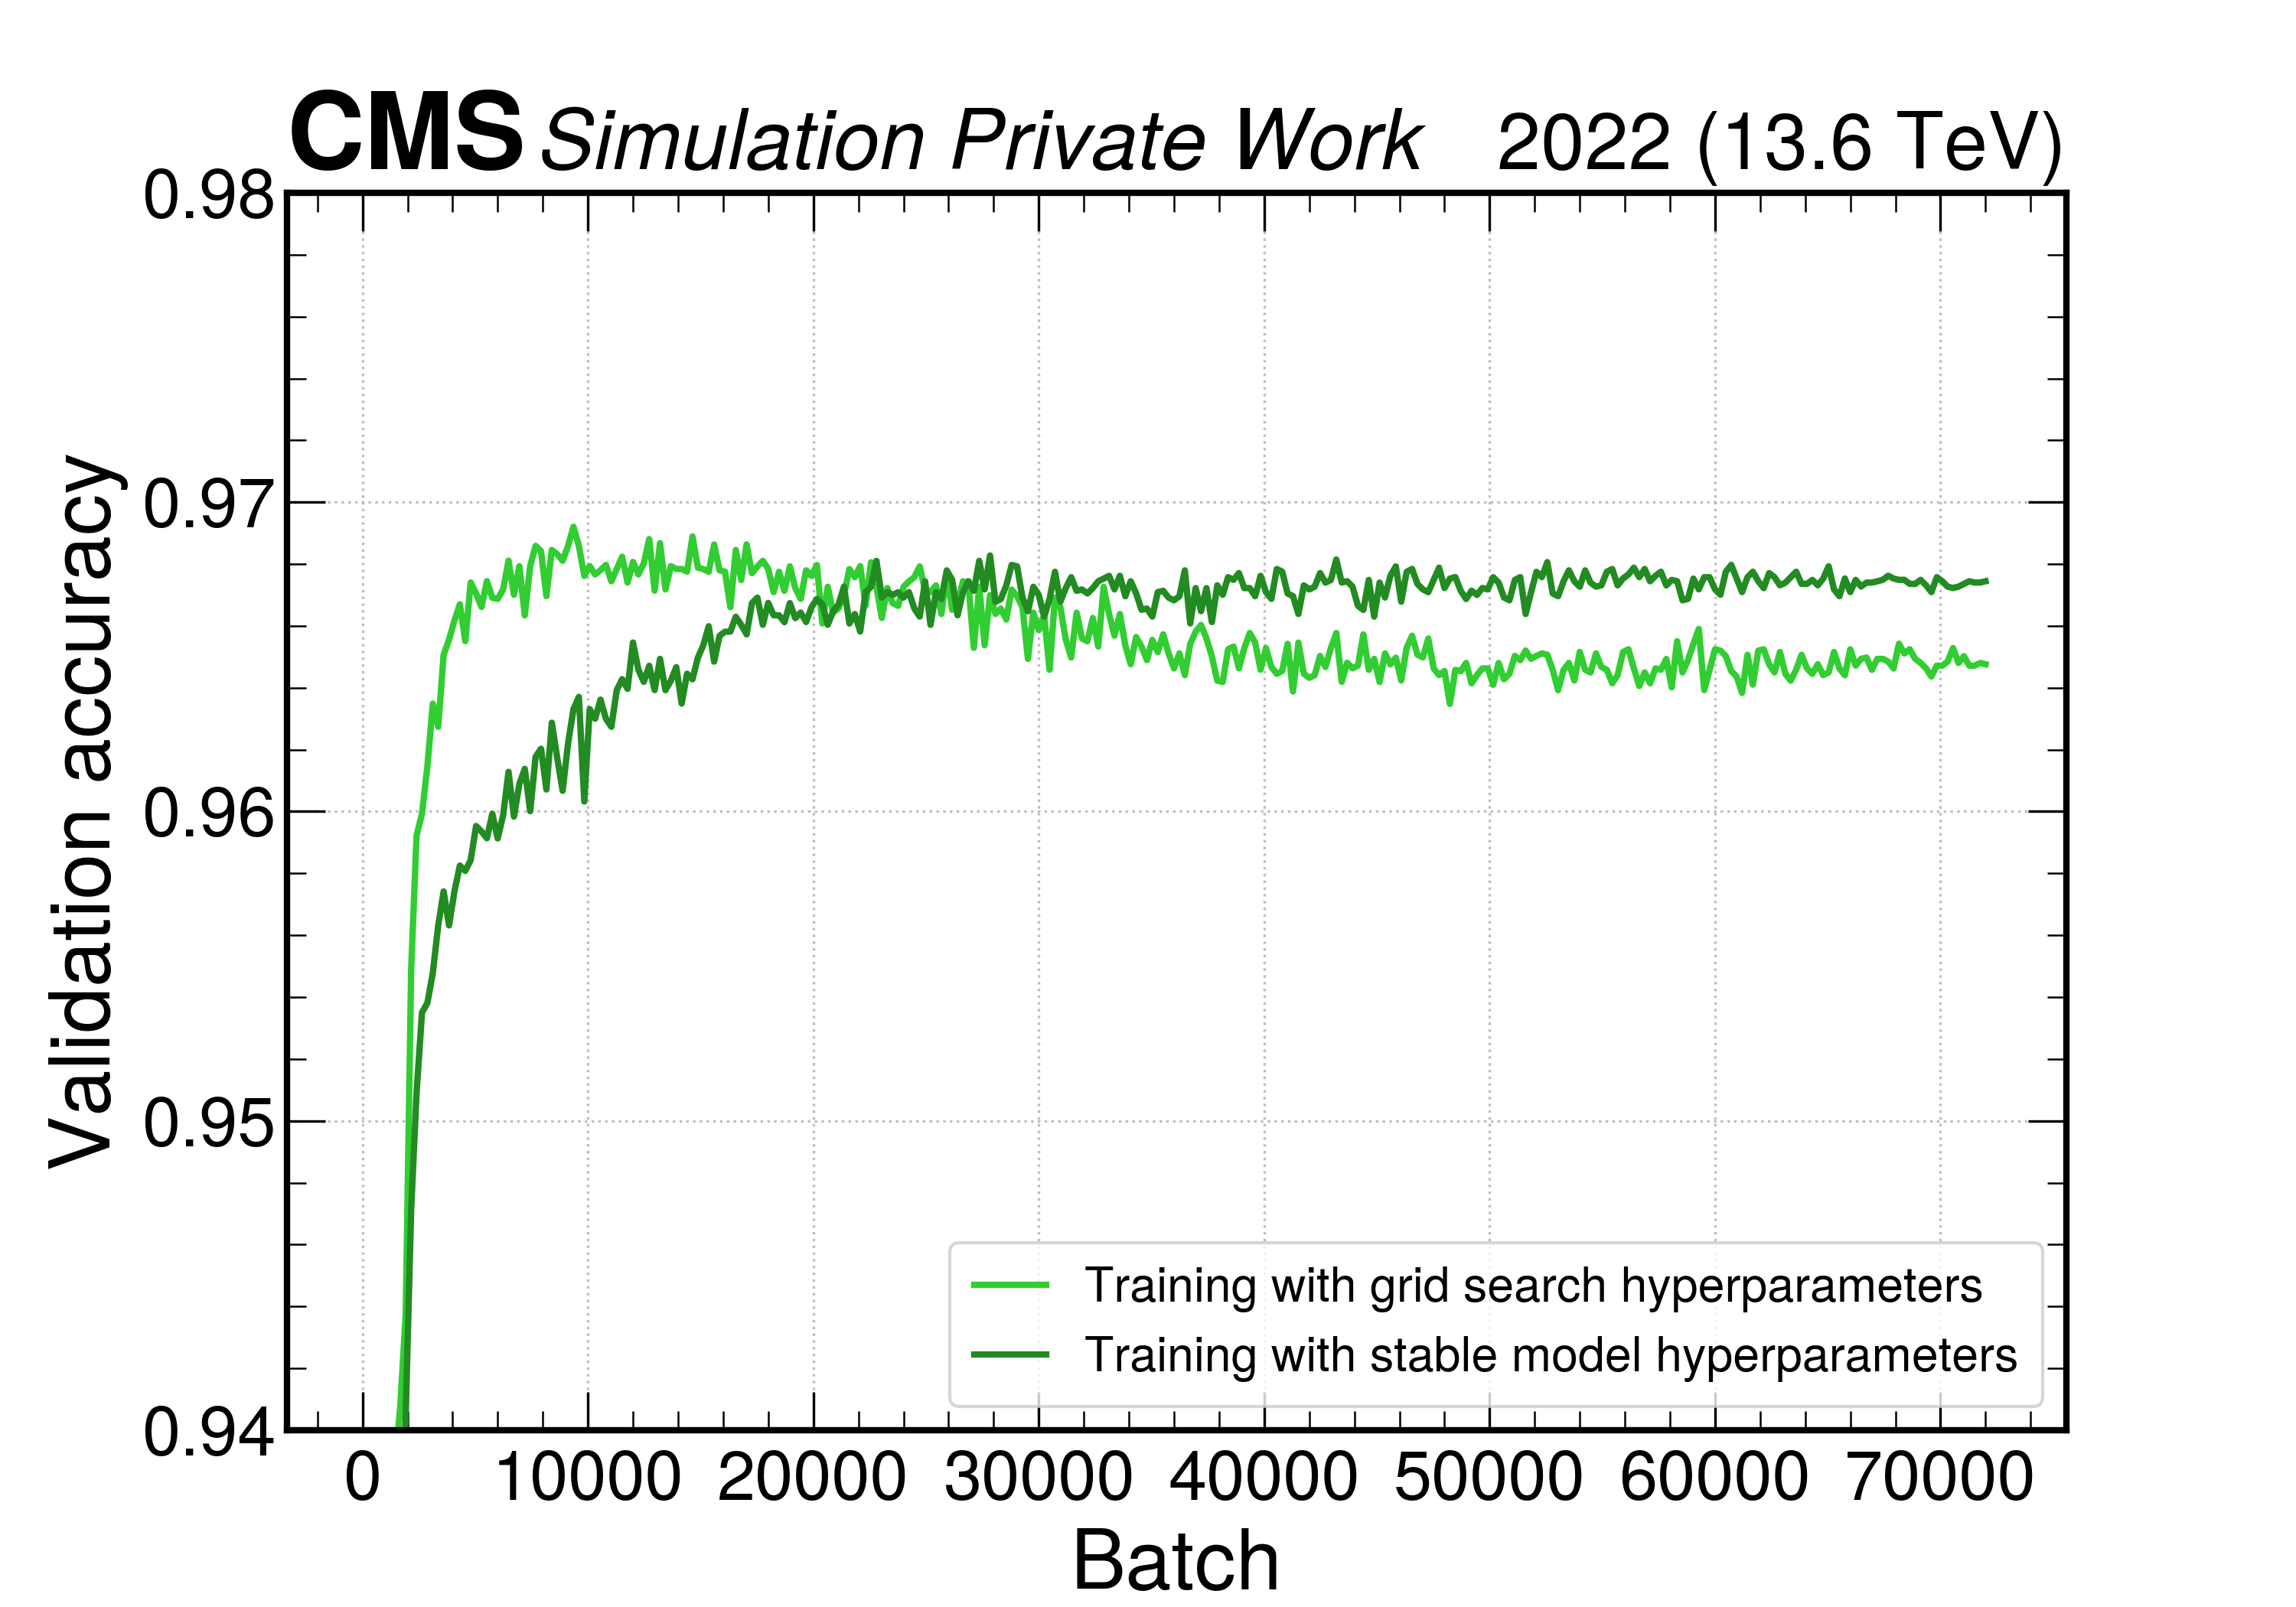
\includegraphics[width=0.6\linewidth]{Images/6.Improving/Grid search/grid search.png}
    \caption{Comparison of the training using the Stable model parameters and the hyperparameters given by the grid search}
    \label{fig: comp grid search}
\end{figure}

%Do i mention other traiinngs done by Mathieu?

\newpage

\subsection{Introducing \kl in the trainings}

As explained in section \ref{section: HH4b}, by measuring the di-Higgs production we are aiming to study 
the Higgs boson self coupling parameter $\lambda$. We can obtain information about it by measuring the cross-section of the di-Higgs production, as the latter can be parameterized in terms of anomalous Higgs boson couplings $\kappa_\lambda$, where $\kappa_\lambda$ is defined as follows:

\begin{equation}
    \kappa_\lambda=\frac{\lambda_{HHH}}{\lambda^{SM}_{HHH}}
\end{equation}

As can be seen in Figure \ref{fig: mhh dist}, for different \kl the kinematics 
of our process change, therefore it is important to train SPANet accordingly. 
To do so, we will use multiple signal samples with different values of $\kappa_\lambda 
\in \{-2.0, -1.0, 0.0, 0.5, 1.0, 1.5, 2.0, 2.45, 3.0, 3.5, 4.0, 5.0\}$. (Do I specify that we performed a validation study between the private and public samples?)

\begin{figure}[hbt]
    \centering
    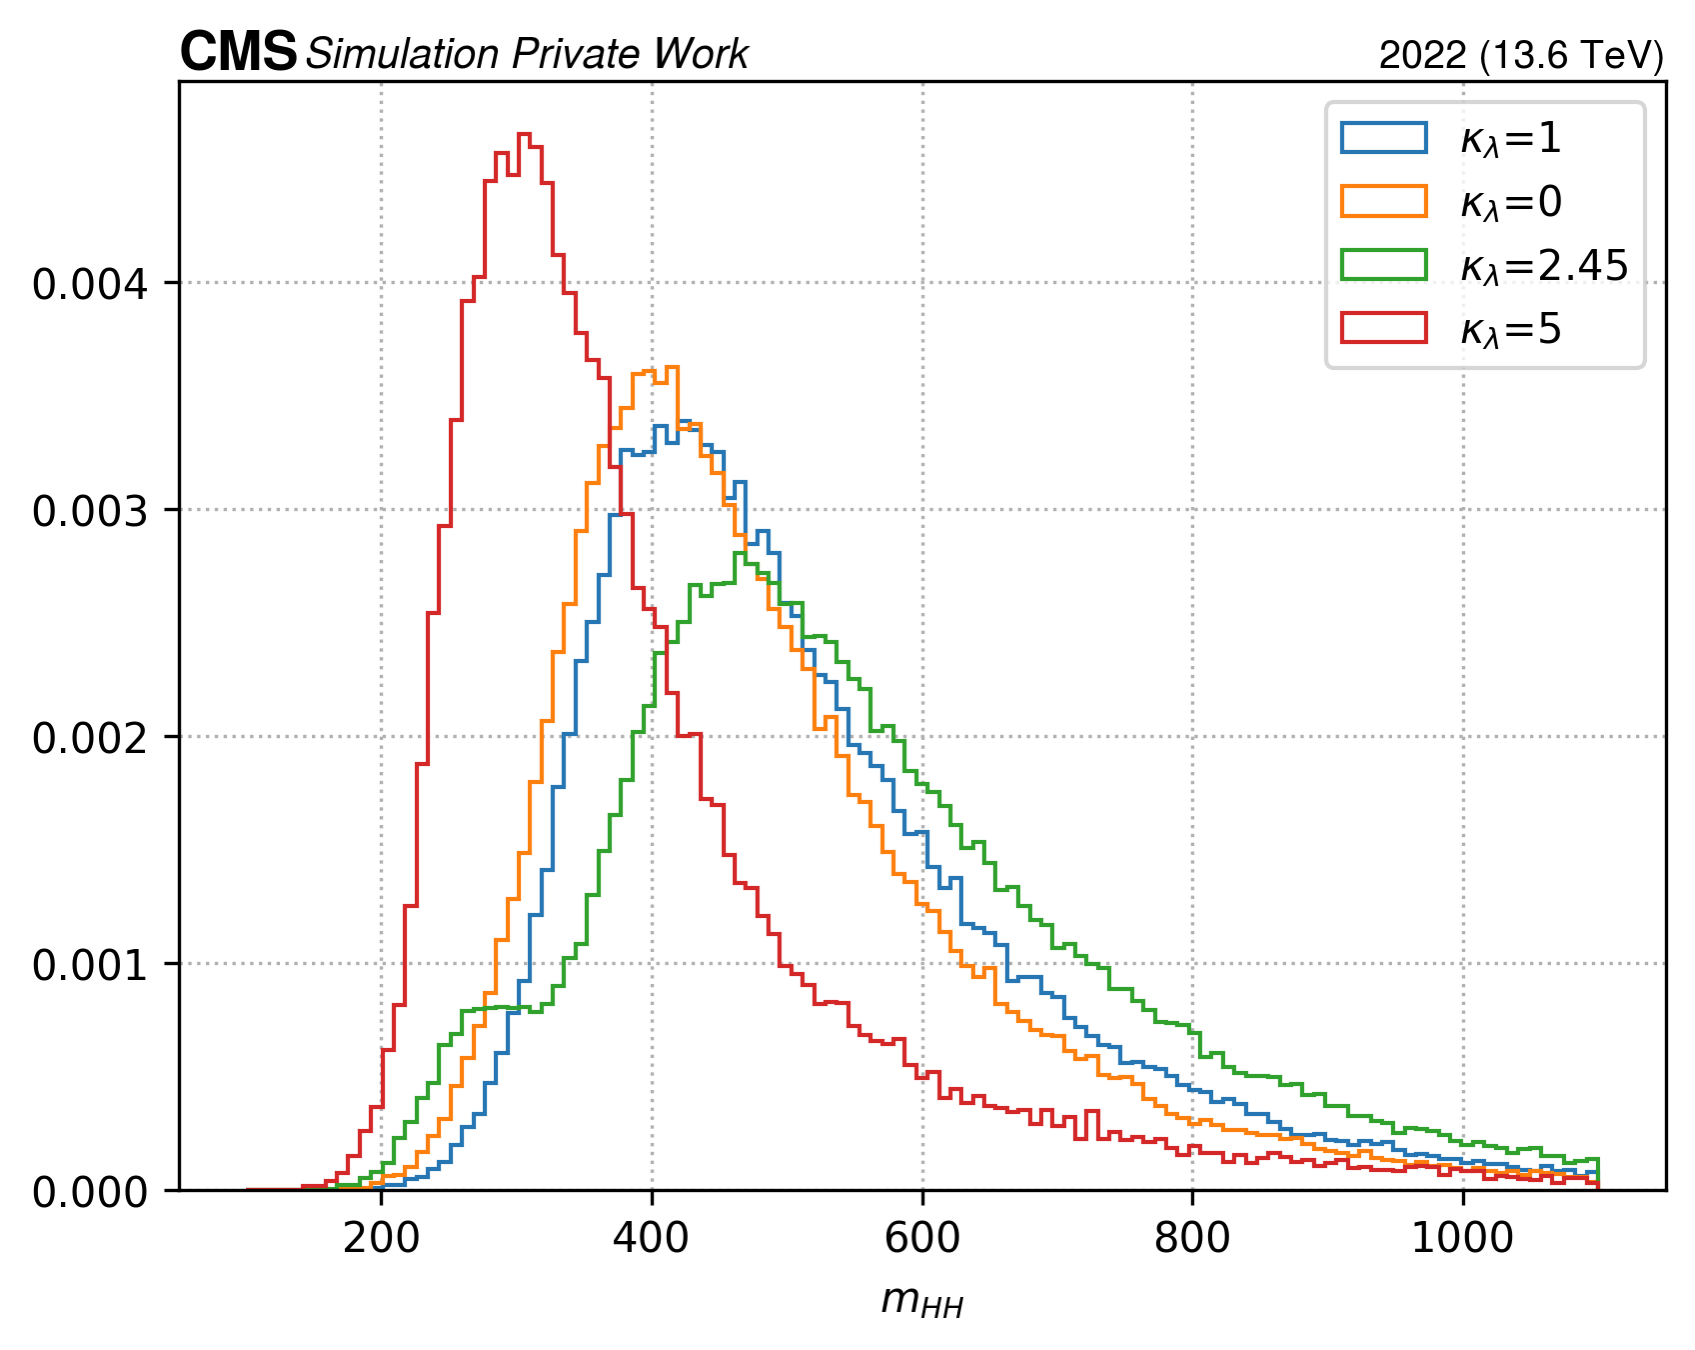
\includegraphics[width=0.5\linewidth]{Images/6.Improving/kappa lambda/mhh distribution for diff kl.png}
    \caption{$m_{HH}$ distribution for different values of \kl}
    \label{fig: mhh dist}
\end{figure}


\vspace{0.2cm}

As described in section \ref{subsection:cutflows}, in our first trainings we started by using the Tight cuts and we always evaluated our model on either Montecarlo or data samples where these cuts were applied. Nevertheless, to have a better comparison to the analysis note (cite), we want to to evaluate our trainings in the Loose cuts as they are the ones used. Therefore, not only we will compare the efficiency of our model trained on samples containing different \kl, but we will also compare the efficiency of our trainings when using the Tight and the Loose cuts.

\noindent We will start by compare the following SPANet models:

\begin{table}[h!]
\centering
\begin{tabular}{|M{2.5cm}|M{6cm}|}
 \hline
 Training  & Configuration  \\
 \hline
  SPANet - \kl - Tight selection &  5 jets as inputs:\footnotesize \begin{itemize}[itemsep=0.001em]
    \item \pt
    \item $\eta$
    \item $\phi$
    \item b-tag
    \item Tight cuts
    \item Train file containing events with different \kl but these are not given as explicit inputs to the network
 \end{itemize}  \\
 \hline
 SPANet - \kl - Loose selection &  5 jets as inputs: \footnotesize \begin{itemize}[itemsep=0.001em]
    \item \pt
    \item $\eta$
    \item $\phi$
    \item b-tag
    \item Loose cuts
    \item Train file containing events with different \kl but these are not given as explicit inputs to the network
 \end{itemize}  \\
 \hline
\end{tabular}
\caption{Configuration of trainings using a sample containing events with different \kl}
\label{table:kl loose vs tight}
\end{table}

In Figure \ref{fig: loose vd tight}, we show the total pairing efficiency differentially in \kl for the trainings presented in Table \ref{table:kl loose vs tight} both evaluated on the test file in which the Loose cuts where applied. We also compare them to the $D_{HH}$-method used in Run 2. From this figure, we can see that the performance is the same for the two trainings within the variability and that they both outperform the $D_{HH}$-method. Nevertheless, if we check the background mass sculpting with these trainings, we can see in Figures \ref{fig: leading H mass dist} and \ref{fig: subleading H mass dist}, that there is quite a significant difference between training with Loose or Tight cuts. Indeed, by training using the Loose cuts it is clear from the figure that for both the Leading and the Subleading Higgs there is much more sculpting of our background. Since this is a feature that we want to avoid for our model, we will stick to the training using Tight cuts but in the next results that will be presented we will always evaluate our model in Loose cuts.

\begin{figure}[hbt]
    \centering
    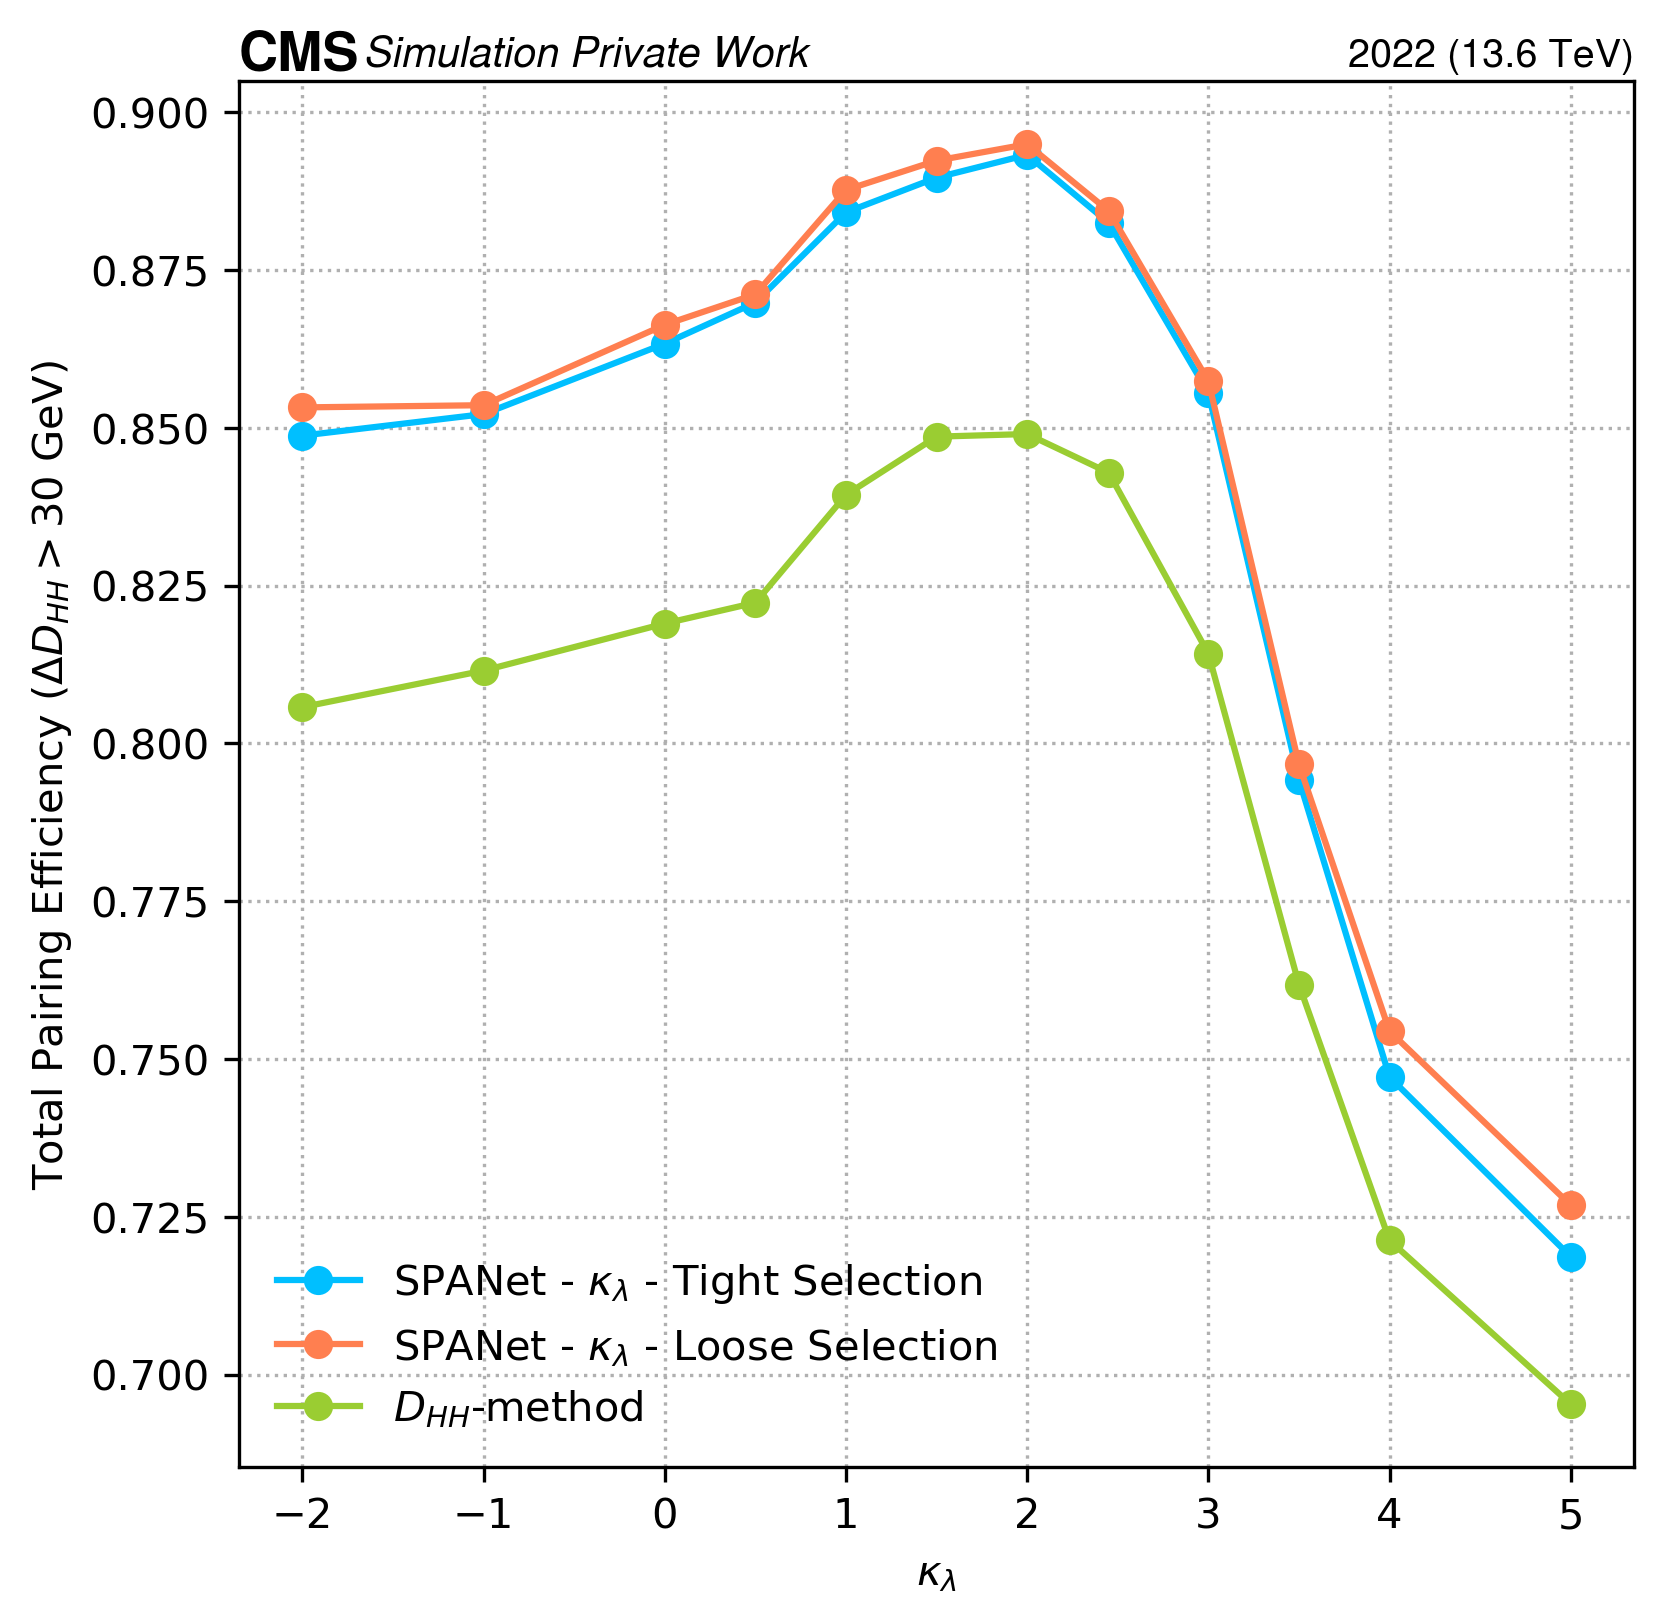
\includegraphics[width=0.6\linewidth]{Images/6.Improving/kappa lambda/loose vs tight.png}
    \caption{Comparison of trainings using Loose or Tight cuts (plot to be re produced)}
    \label{fig: loose vd tight}
\end{figure}

\begin{figure}[hbt]
    \centering
    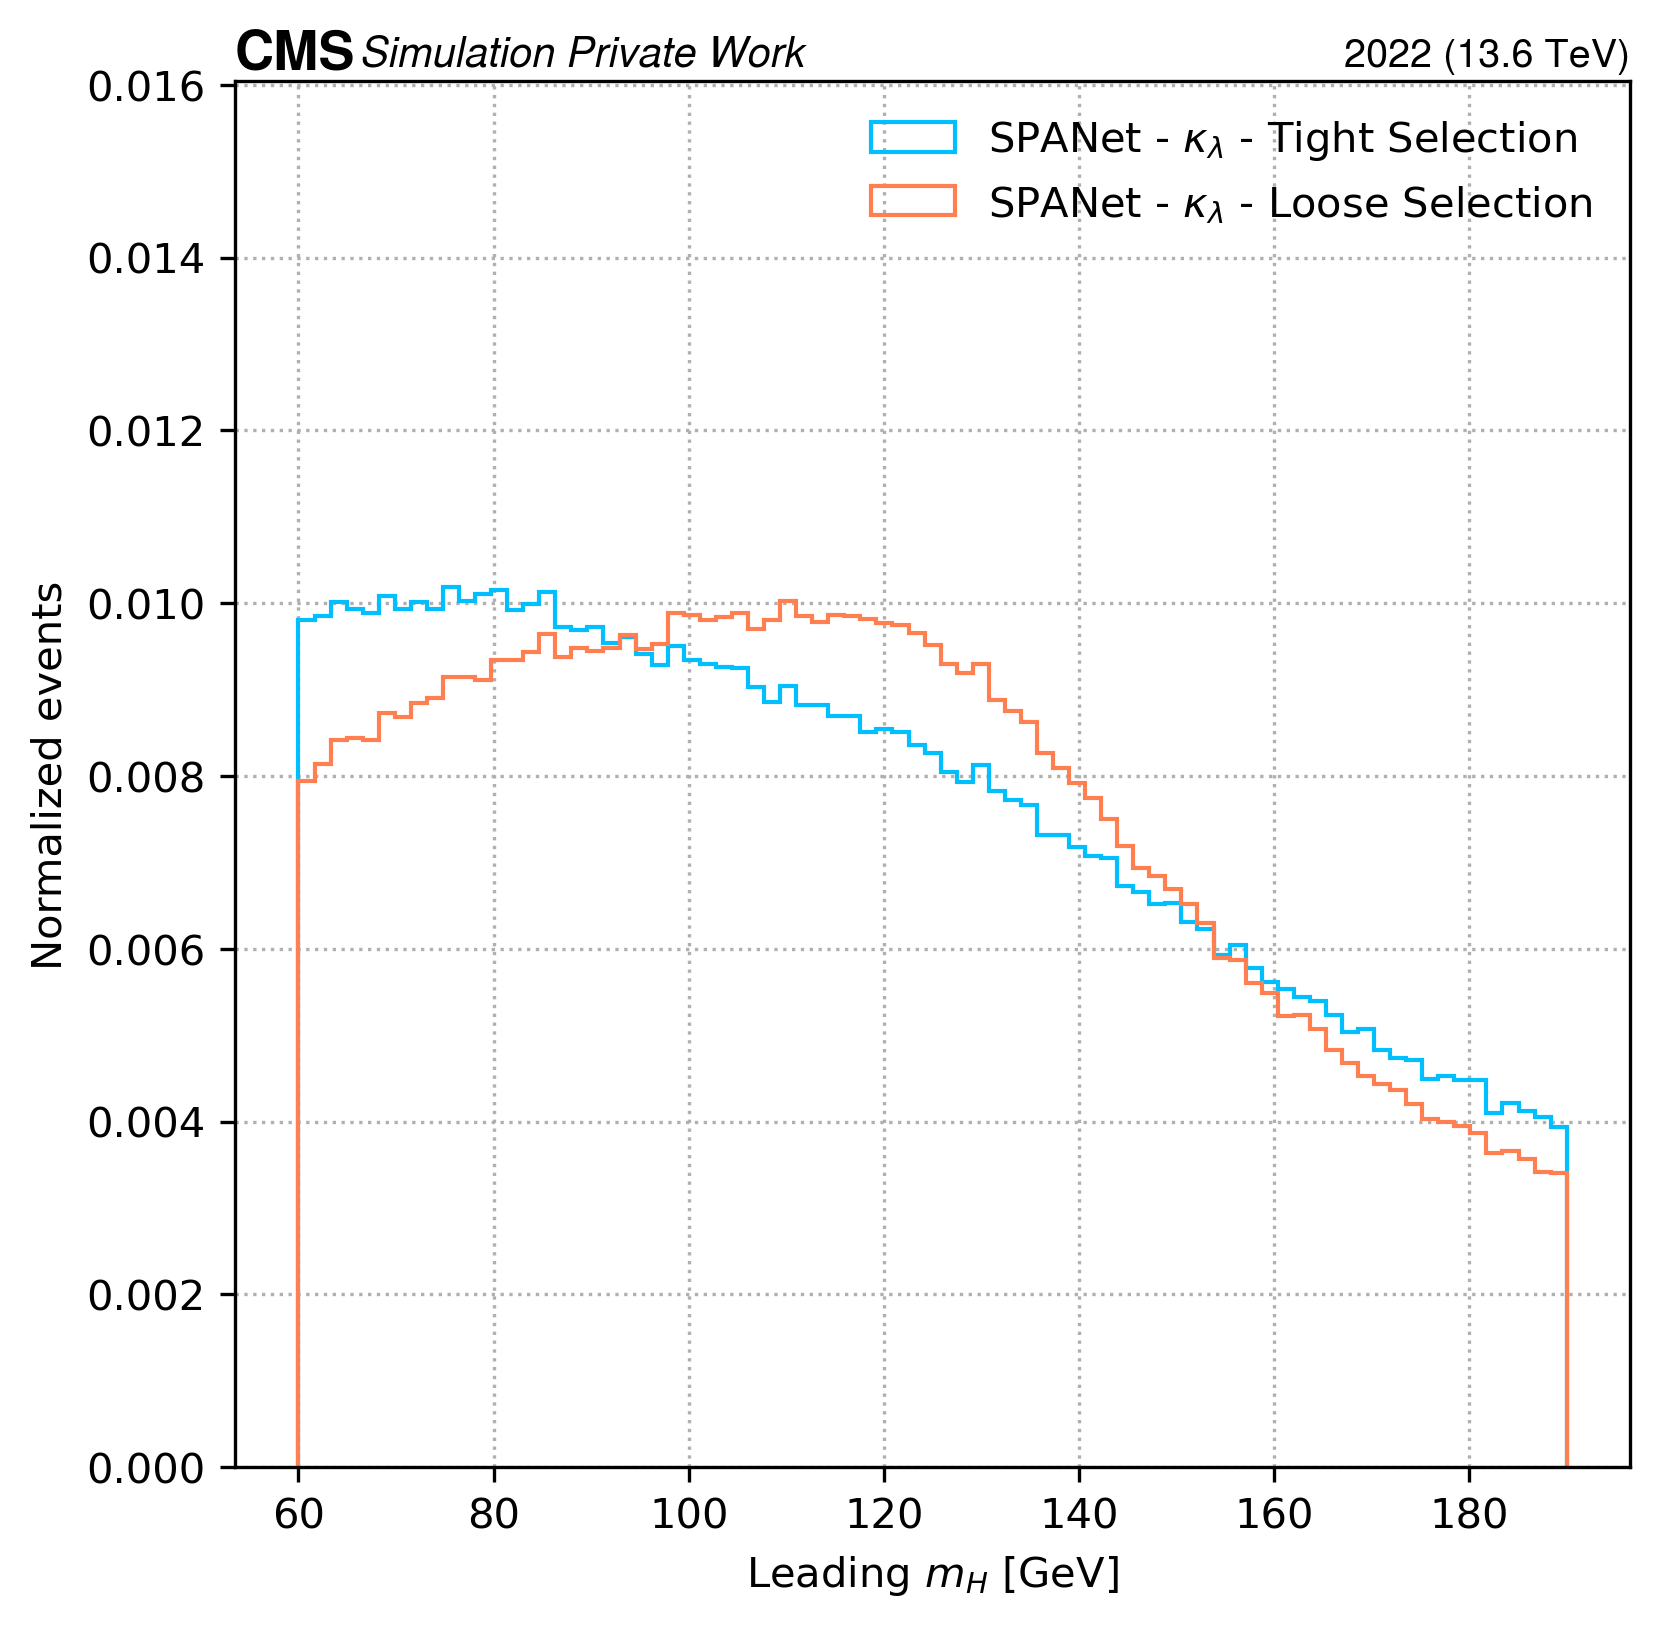
\includegraphics[width=0.6\linewidth]{Images/6.Improving/kappa lambda/leading h mass sculp.png}
    \caption{1D mass distribution of the leading Higgs (To be reproduced)}
    \label{fig: leading H mass dist}
\end{figure}

\begin{figure}[hbt]
    \centering
    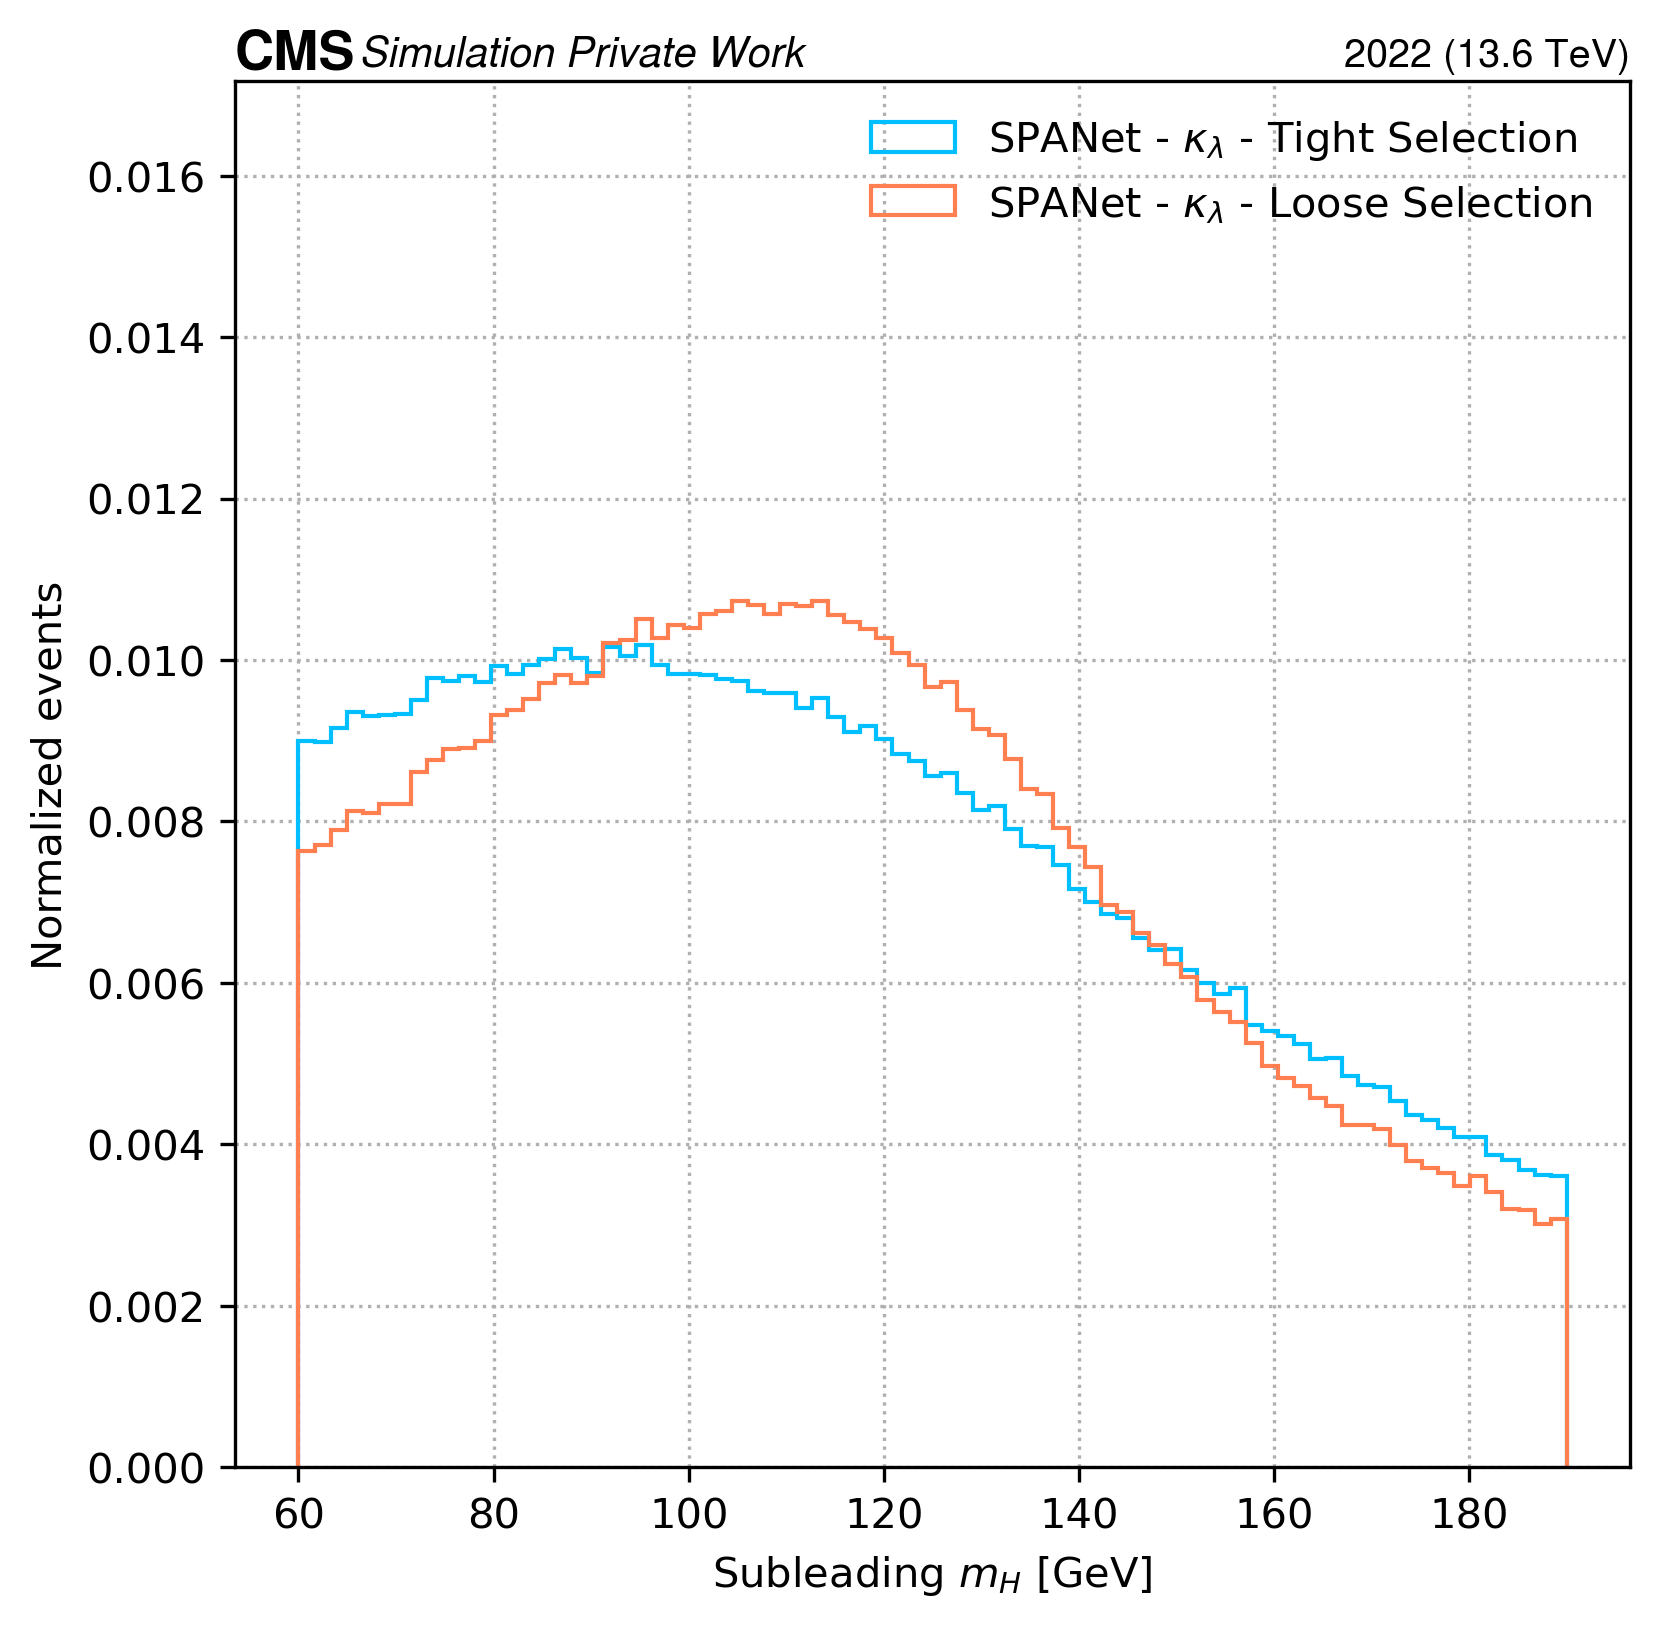
\includegraphics[width=0.6\linewidth]{Images/6.Improving/kappa lambda/sub leading H mass sculpt.png}
    \caption{1D mass distribution of the subleading Higgs (To be reproduced)}
    \label{fig: subleading H mass dist}
\end{figure}

The next feature we wanted to check regarding trainings with \kl is how much does the efficiency change when including the \kl explicitly as global inputs in our model. Hence, we will be comparing the total pairing efficiency differencially in \kl and in $m_{HH}$ of the models presented in Table \ref{table:kl as input or not}.

\begin{table}[h!]
\centering
    \begin{tabular}{|M{4cm}|M{7cm}|}
     \hline
     Training  & Configuration \\
     
     \hline
     
    SPANet - \kl - Tight selection &  5 jets as inputs:\footnotesize 
    \begin{itemize}[itemsep=0.001em]
        \item \pt
        \item $\eta$
        \item $\phi$
        \item b-tag
        \item Tight cuts
        \item Train file containing events with different 
        \item \kl not an explicit input to the network
    \end{itemize} \\
     
     \hline
     
    SPANet - \kl (\kl inputs)- Tight selection &  5 jets as inputs: \footnotesize 
    \begin{itemize}[itemsep=0.001em]
        \item \pt
        \item $\eta$
        \item $\phi$
        \item b-tag
        \item Loose cuts
        \item Train file containing events with different \kl
        \item \kl as global input
    \end{itemize} \\
     
     \hline
     
      SPANet - SM - Tight selection &  5 jets as inputs: \footnotesize 
    \begin{itemize}[itemsep=0.001em]
        \item \pt
        \item $\eta$
        \item $\phi$
        \item b-tag
        \item Tight cuts
        \item Train file containing only events with SM coupling 
    \end{itemize}\\
    
    
     \hline
    \end{tabular}
    \caption{Configuration of trainings using a sample containing events with different \kl}
    \label{table:kl as input or not}
\end{table}

In Figures \ref{fig: kl kl input or no input} and \ref{fig: mhh kl input or no input}, we can see the results of this comparison. Firstly, we show in Figure \ref{fig: kl kl input or no input} the total pairing efficiency differencially in \kl.
We find that by training our model using a sample with different \kl, our performance is improved. However, using \kl as an explicit input to our network does not improve our performance. The same conclusion can be drawn from Figure \ref{fig: mhh kl input or no input}, where we show the total pairing efficiency differencially in $m_{HH}$. Especially in the low $m_{HH}$ mass region, we can see a big improvement compared to the trainings using only SM samples. Finally, in both figures one finds that the pairing efficiency using the $D_{HH}$-method is outperformed.

\begin{figure}[hbt]
    \centering
    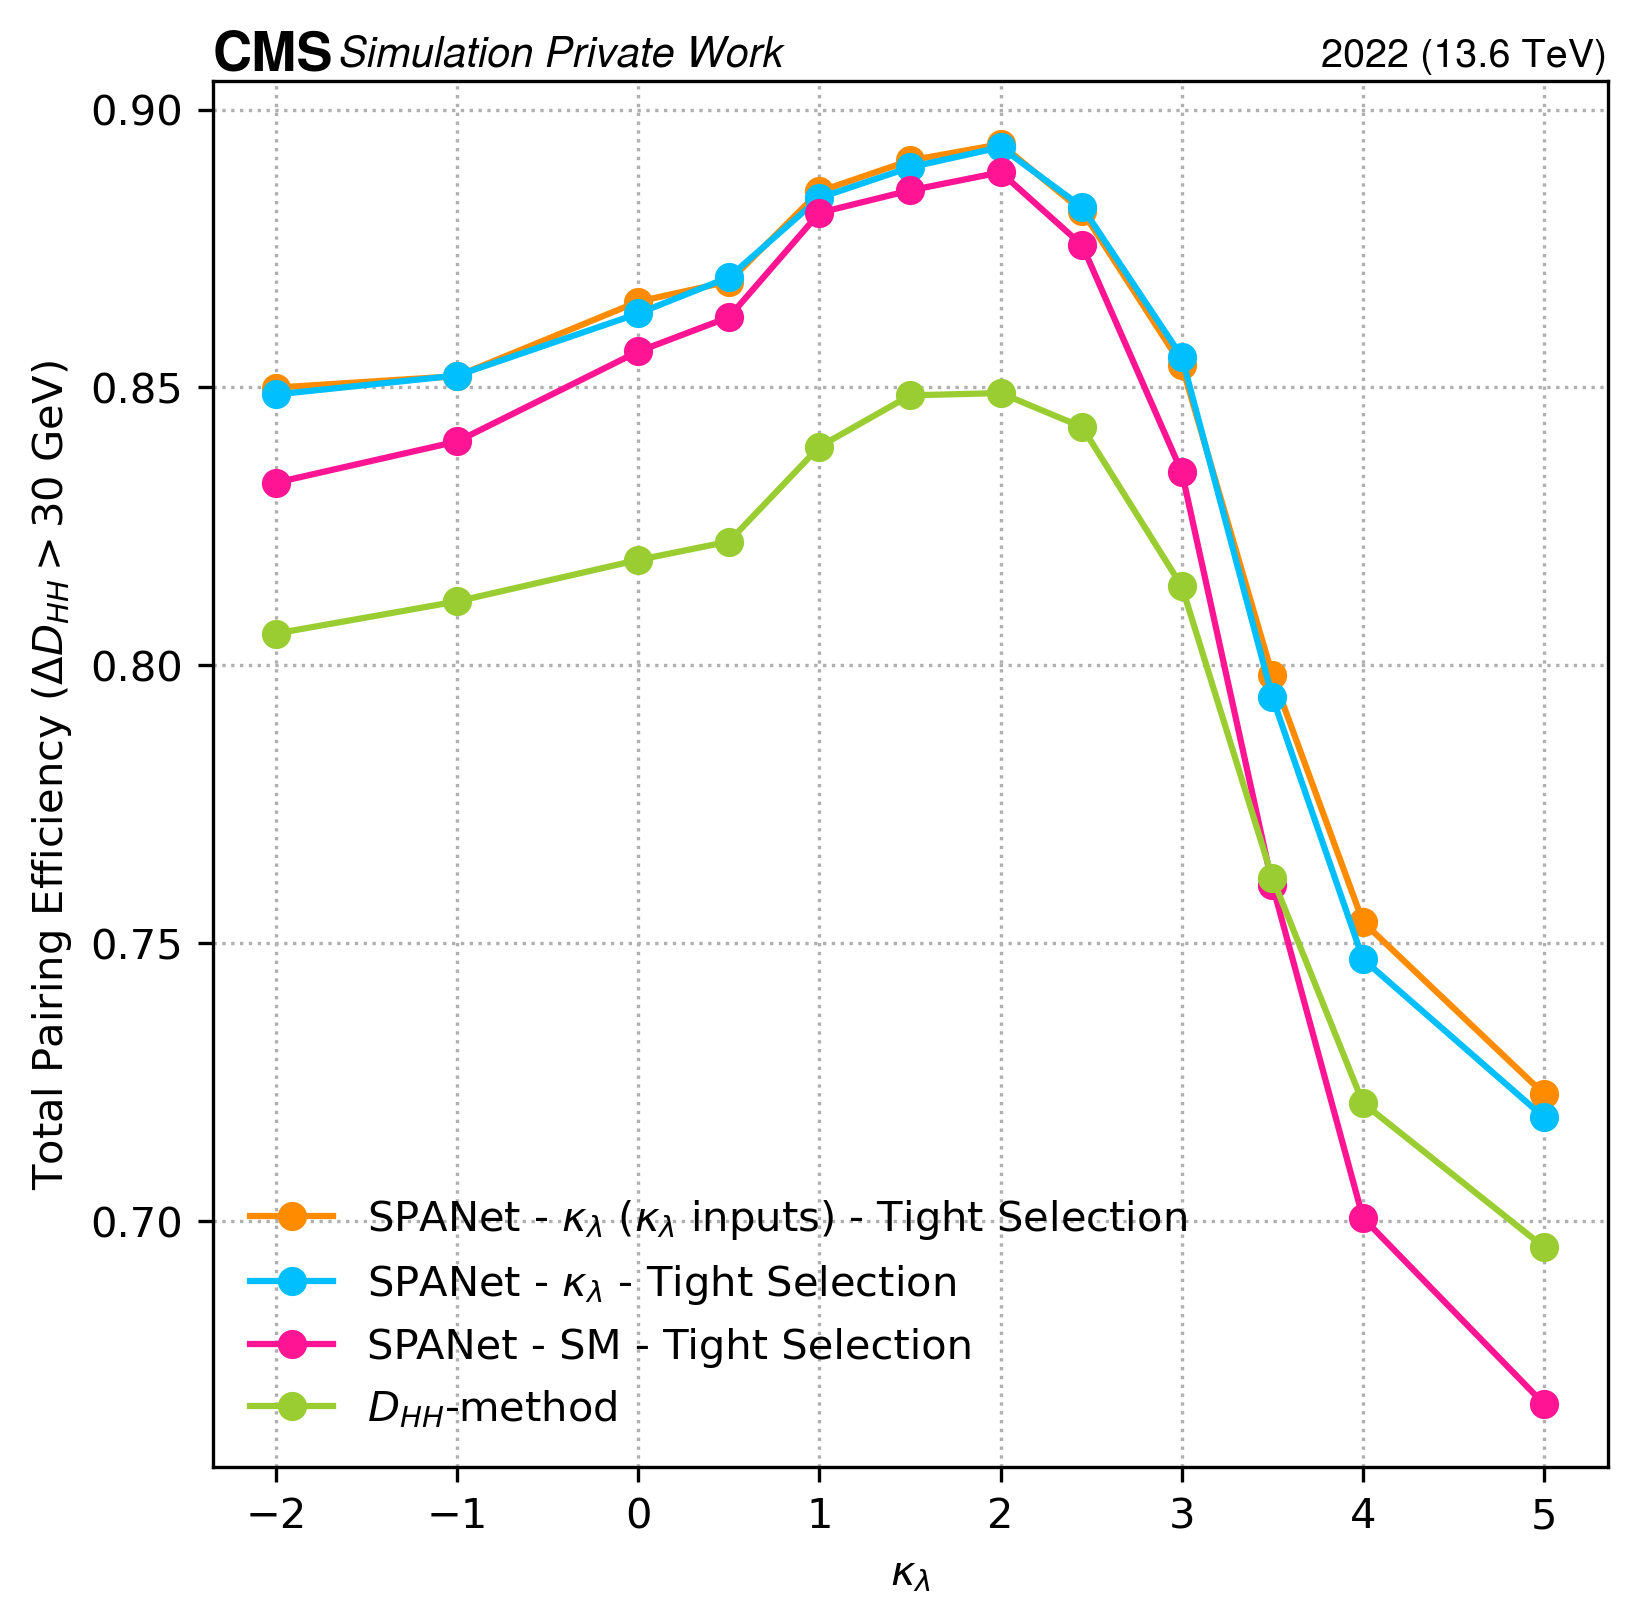
\includegraphics[width=0.6\linewidth]{Images/6.Improving/kappa lambda/kl inout vs no input.png}
    \caption{Total pairing efficiency differencially in \kl (To be reproduced)}
    \label{fig: kl kl input or no input}
\end{figure}

\begin{figure}[hbt]
    \centering
    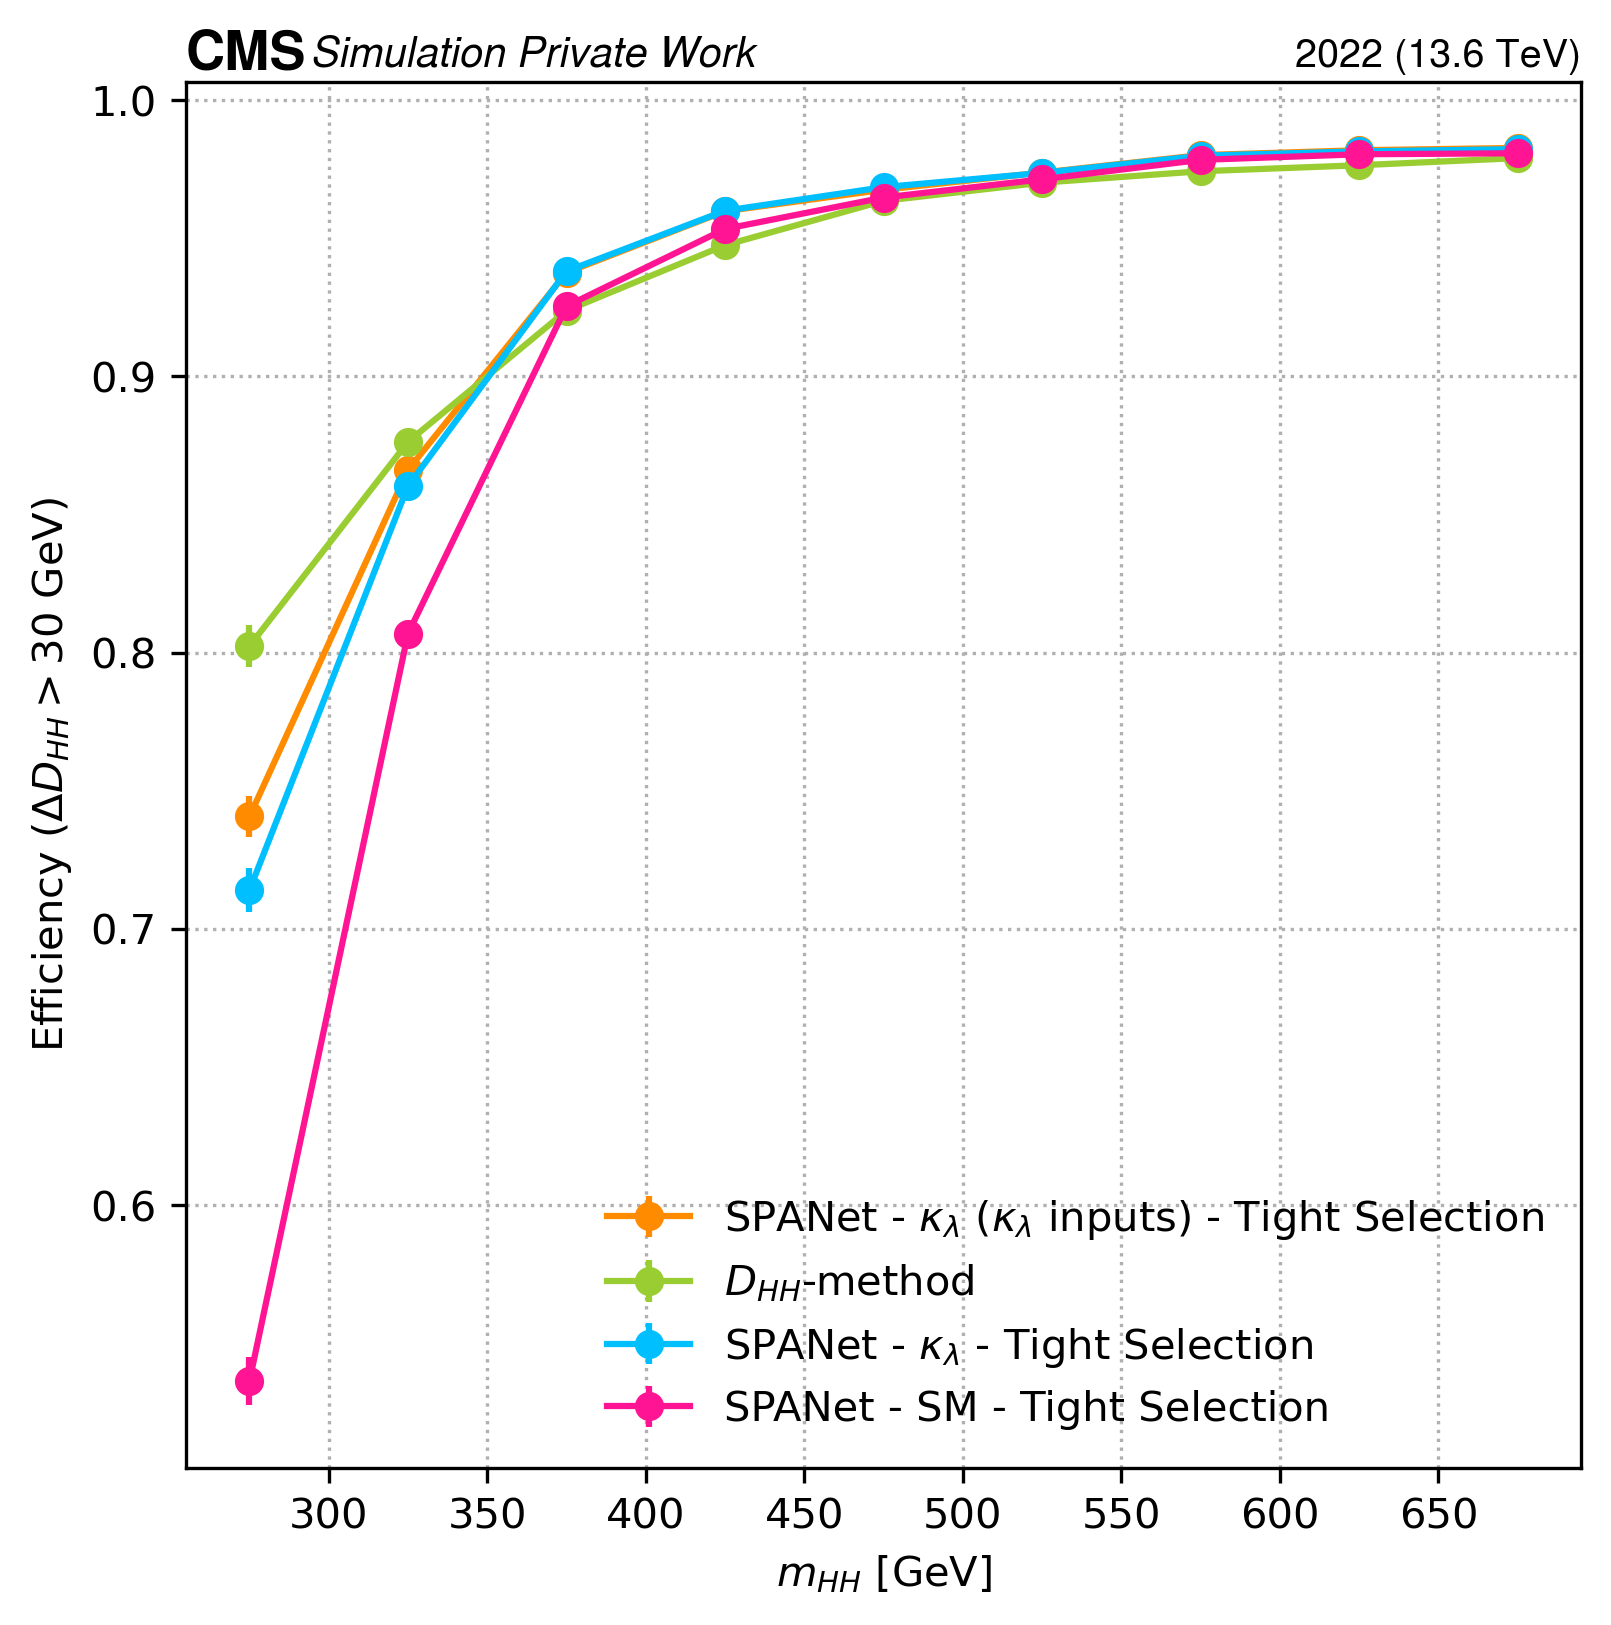
\includegraphics[width=0.6\linewidth]{Images/6.Improving/kappa lambda/eff diff kl vs kl input.png}
    \caption{Total pairing efficiency differencially in $m_{HH}$ (To be reproduced)}
    \label{fig: mhh kl input or no input}
\end{figure}



Since we concluded from these figures that adding \kl as an explicit input does not improve our efficiency, we will use the model where we don't explicitly add \kl as input since when we are evaluating our model on data, we can't know to which \kl corresponds each event. Therefore, since if we evaluate our model on either data or QCD it would be ambiguous what to give to \kl as input, we decide to stick to the SPANet - \kl - Tight selection model.

In Table \ref{table: improvement} we show the values of the pairing efficiency as well as the total pairing efficiency for \kl $\in \{ 0 , 1 , 5 \} $ with our best model. From these values we see that by using the training SPANet - \kl - Tight selection, we have \textbf{4-8\%} absolute improvement with respect to the $D_{HH}$-method, as well as a \textbf{5-14\%} relative improvement ! 

\begin{table}[h!]
\centering
\begin{tabular}{|M{2.5cm}||M{1.75cm}|M{1.75cm}||M{1.75cm}|M{1.75cm}||M{1.75cm}|M{1.75cm}|}
 \hline
 Training  & Pairing efficiency (\kl=1) &  Total pairing efficiency (\kl=1) & Pairing efficiency (\kl=0) &  Total pairing efficiency (\kl=0) & Pairing efficiency (\kl=5) &  Total pairing efficiency (\kl=5) \\
 \hline
  $D_{HH}$-method &  0.944 &  0.836 & 0.921 & 0.808 & 0.739 & 0.603\\
 \hline
 SPANet - \kl - Tight selection & 0.952  &  0.880 & 0.932 & 0.853 & 0.792 & 0.685 \\
 \hline
\end{tabular}
\caption{Comparison of the pairing efficiency and the total pairing efficiency between the $D_{HH}$-method and the training SPANet - \kl - Tight selection}
\label{table: improvement}
\end{table}

As a final check for this model, we show the 2D mass sculpting of the background. As can be seen in Figure \ref{fig: 2D mass dist kl}, we don't observe any excess of peaks in the signal region.

\begin{figure}
    \centering
    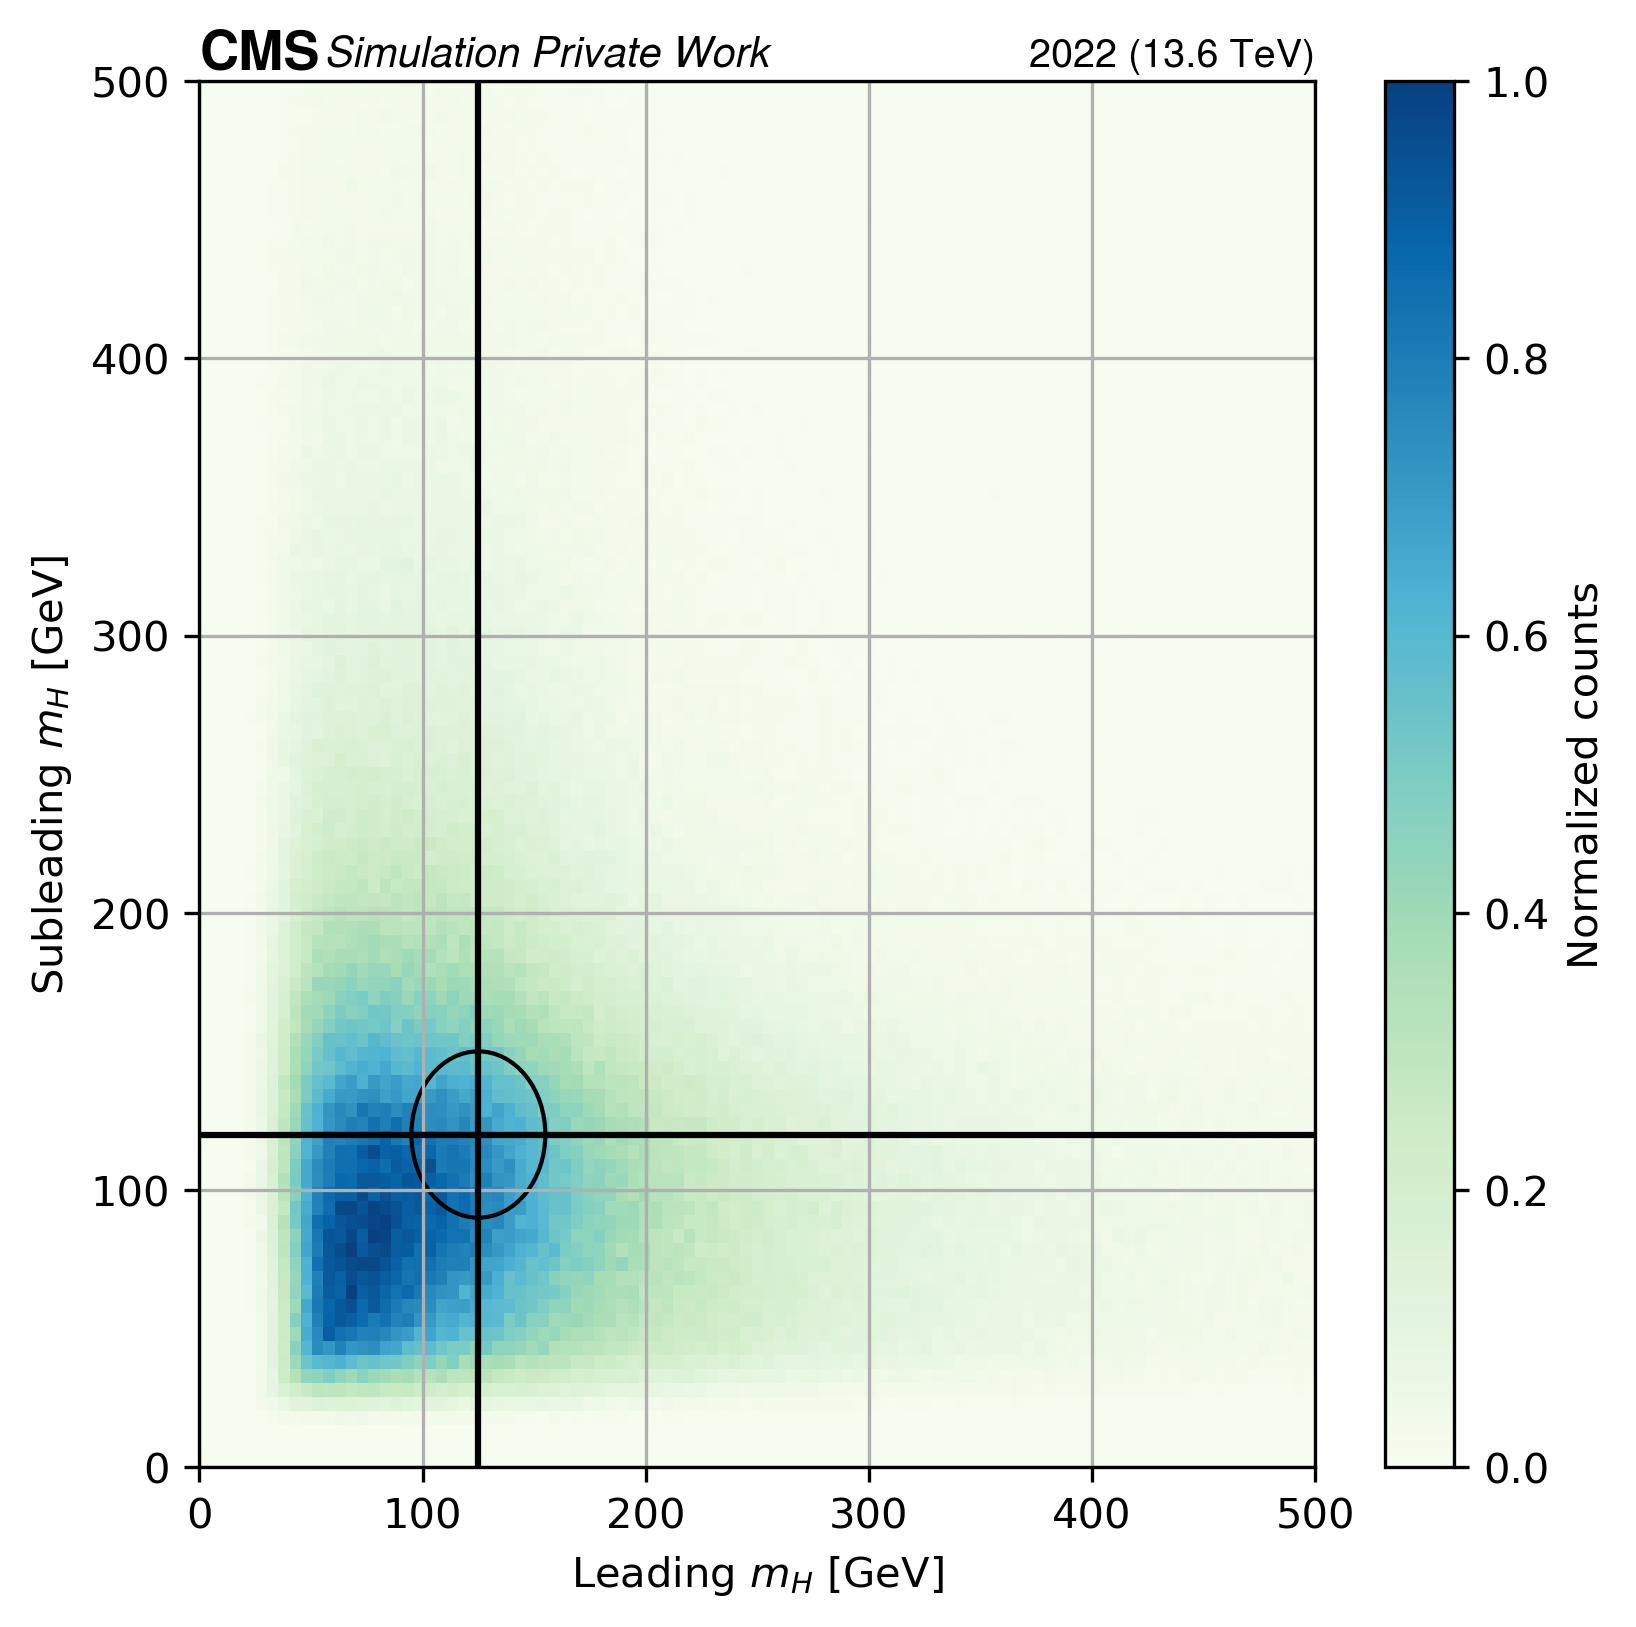
\includegraphics[width=0.6\linewidth]{Images/6.Improving/kappa lambda/mass dist best model.png}
    \caption{2D mass distribution of the  SPANet - \kl - Tight selection model evaluated on 2b data (To be reproduced)}
    \label{fig: 2D mass dist kl}
\end{figure}

\clearpage

\subsection{The final configuration}
After comparing several configurations, we conclude that the best performance for jet pairing is given by the SPANet - \kl - Tight selection model which uses 5 jets as sequential inputs (with \pt reg, $\eta$, $\phi$ and b-tag), no explicit \kl input as global variable as well as the hyperparameters of the stable model shown in Table \ref{table: stable model}.

% jets as inputs, pt reg, lite and stable model, tight cuts, no kl as inout explicitely

\section{S/B classification}

loss function weights
Direction for comparisons:
		1) architecture
		2) input features
		3) sample dependency
		4) for background from MC weight vs no weights


\section{Conclusion}

This thesis introduces the usage of SPANet, an attention-based neural network, for the HH $\to$ 4b analysis. Section \ref{section: improving} presents the results of using SPANet to find the best pairing between the reconstructed jets and the generator-level quarks and Section \ref{section: s/b classification} reports the results of using SPANet as a signal/background classifier.

\vspace{0.2 cm}

Regarding the pairing efficiency, we converged on the model that showed the highest pairing efficiency, the least background sculpting, and the smallest variability. To determine this model, first, the jet multiplicity for the training was assessed. Then, different SPANet hyperparameters and input variables were tested to find the model with the highest pairing efficiency. After finding the best two performing models, the background mass sculpting was verified and one of the two was selected. Nevertheless, due to the instability of this training with respect to the validation accuracy, the SPANet architecture had to be further modified until the hyperparameters gave rise to a more stable model. Moreover, different trainings were tested using samples with different values of $\kl$ to verify the pairing efficiency as a function of \kl. It was concluded that training the model with samples containing $\kl$ samples improved the pairing efficiency as a function of \kl and $m_{HH}$. Adding \kl explicitly as a global input did not improve the performance, therefore it was decided to not include it. Finally, the impact of different kinematic selections in the analysis was tested, i.e. using Tight or Loose cuts (Section \ref{section: HH4b}) in the training samples. It was shown that using Tight cuts for the training led to a higher pairing efficiency and less background mass sculpting. Thus, in conclusion, the SPANet model that we converged on is the SPANet - \kl - Tight selection model that uses:
\begin{itemize}
    \item \pt regressed, $\eta$, $\phi$ and b-tag of the 5 jets considered for the pairing as sequential inputs
    \item No explicit \kl input as a global variable
    \item Stable model hyperparameters (shown in Table \ref{table: stable model})
\end{itemize}
\noindent Not only this model has the best pairing efficiency among all the ones tested, but it also outperforms the pairing efficiency of the $D_{HH}$-method used in the Run 2 analysis.

\vspace{0.2 cm}

When using SPANet as a S/B classifier, signal and background samples were used for the training. Therefore, the loss function needs to be modified and to do so, event and class weights were introduced in the computation. These allow to properly account for MC production effects and the difference in the number of signal and background events and thus avoid imbalance classification problems. Ideally, the background sample for the training would be 4b-morphed data (Section \ref{section: HH4b}). Nevertheless, as it is not possible to use it at the moment, different training configurations were tested using 2b-data, 4b-data, and 4b-QCD background samples (Section \ref{section: HH4b}) in order to infer the results for 4b-data using Eq.(\ref{eq: extrapolation}). For each background configuration, different inputs were tested: either the so-called "DNN" and "Probability Difference" (PD) variables, defined in Section \ref{section: s/b classification}, or uniquely DNN variables.  To assess the performance of the trainings, the ROC curves and the AUC values were compared. The variability of the different trainings was assessed as well, and a large variability was observed for the configuration using the 4b-QCD sample. This leads to variability for the inferred 4b-data results, and the results from the DNN used for Run 3 data are then compared within this observed variability. Finally, to have a better comparison to the DNN used for the Run 3 analysis, it was decided to train and evaluate the SPANet models on SR samples. It was concluded that the DNN for Run 3 is outperformed by the novel SPANet training using the DNN and the PD variables up to 85\% signal efficiency. After this 85\% signal efficiency, the probability distribution given by SPANet is dominated by the background (Figure \ref{fig: Assigned prob 4b QCD SR}), and the SR samples used have very few statistics. Thus the oversampling of the 4b-QCD-SR sample is proposed to compare the performance of the inferred 4b-data ROC curve to the ROC curve of the DNN for Run 3. Finally, as a next step, to further test the performance of SPANet for the classification, it is proposed to train the model using 4b-morphed data. 

\section*{Acknowledgements}

%My basketball buddy

% \bibliography{bibliography}
% \bibliographystyle{plain}

\printbibliography

\end{document}
